\documentclass[10pt,a4paper,oneside]{book}

% course info (for title)
\newcommand{\courseid}{PHYS 273}
\newcommand{\coursetitle}{Waves and Oscillations}
\newcommand{\semester}{Fall 2024}
\newcommand{\credit}{Adapted from 
    PHYS273 lectures.}  

\usepackage[utf8]{inputenc}
\usepackage[margin=1.0in]{geometry}
\usepackage{amsmath}
\usepackage{amsfonts}
\usepackage{amssymb}
\usepackage{enumitem}                       % custom enum labels
\usepackage{parskip}                        % add vertical paragraph space
\usepackage{tocloft}						% modify toc position
\usepackage{xr}								% cross-references
\usepackage{mathtools}						% Aboxed
\usepackage{empheq}							% box multiple lines
\usepackage{upgreek}
\usepackage{siunitx}
\usepackage{chemformula}
\usepackage{esint}							% oiint
\usepackage{cancel}
\usepackage{bm}
\usepackage{physics}
\usepackage[framemethod=TikZ]{mdframed}     % graphics and framed envs
\usepackage[hang,flushmargin]{footmisc}		% remove footnote indentation
\usepackage[hyperfootnotes=false,
					hidelinks]{hyperref}	% create clickable table of contents


\renewcommand{\familydefault}{\sfdefault}  	% sans serifs text
\setlength{\parindent}{0pt}                	% no paragraph indentation

\AtBeginDocument{\RenewCommandCopy\qty\SI} 
 
% region TITLES
\setbox0=\hbox{\Huge{\textbf{\textsf{\courseid: }}}}
\setlength{\cftbeforetoctitleskip}{0em}
\setlength{\cftaftertoctitleskip}{1em}
\renewcommand{\contentsname}{\hangindent=\wd0 \strut \courseid: \coursetitle \\ \medskip \LARGE{Isabelle, \semester}}

\let\footnoterule\relax
\newcommand\blfootnote[1]{%
  \begingroup
  \renewcommand\thefootnote{}\footnote{#1}%
  \addtocounter{footnote}{-1}%
  \endgroup
}

\usepackage{titlesec}
\titleformat{\chapter}{\Huge\normalfont\bfseries}{\thechapter}{1em}{}
\titlespacing*{\chapter}{0em}{0em}{2em}
% endregion

\let\oldphi = \phi
\let\phi = \varphi

% region COMMANDS
\newcommand{\ds}{\displaystyle}
\newcommand{\pfn}[1]{\textrm{#1}}	% enables new functions
\newcommand{\mbf}[1]{\mathbf{#1}}	% mathbf
\newcommand{\C}{\mathbb{C}}			% fancy C
\newcommand{\R}{\mathbb{R}}			% fancy R
\newcommand{\Q}{\mathbb{Q}}			% fancy Q
\newcommand{\Z}{\mathbb{Z}}			% fancy Z
\newcommand{\N}{\mathbb{N}}			% fancy N
\newcommand{\from}{\leftarrow}
\newcommand{\qed}{$\square$}
\newcommand{\xhat}{\mbf{\hat{x}}}
\newcommand{\yhat}{\mbf{\hat{y}}}
\newcommand{\zhat}{\mbf{\hat{z}}}
\newcommand{\phihat}{\bm{\hat{\phi}}}
\newcommand{\rhat}{\mbf{\hat{r}}}
\newcommand{\dotunit}[1]{\bm{\dot{\hat{#1}}}}
\newcommand{\ddotunit}[1]{\bm{\ddot{\hat{#1}}}}
\renewcommand{\it}[1]{\textit{#1}}
\renewcommand{\bf}[1]{\textbf{#1}}
\renewcommand\pmat[1]{\begin{pmatrix}#1\end{pmatrix}} 
\newcommand\vmat[1]{\begin{vmatrix}#1\end{vmatrix}}
\newcommand\bmat[1]{\begin{bmatrix}#1\end{bmatrix}}
\newcommand{\mcl}[1]{\mathcal{#1}}
\renewcommand{\L}{\mcl{L}}
% endregion

% region ENVIRONMENTS
\newcounter{theo}[chapter]\setcounter{theo}{0}
\newcommand{\numTheo}{\arabic{chapter}.\arabic{theo}}
\newcommand{\mdftheo}[3]{
	\mdfsetup{
		frametitle={
			\tikz[baseline=(current bounding box.east),outer sep=0pt]
			\node[anchor=east,rectangle,fill=#3]
			{\ifstrempty{#2}{\strut #1~\numTheo}{\strut #1~\numTheo:~#2}};
		},
		innertopmargin=4pt,linecolor=#3,linewidth=2pt,
		frametitleaboveskip=\dimexpr-\ht\strutbox\relax,
		skipabove=11pt,skipbelow=0pt
	}
}
\newcommand{\mdfnontheo}[3]{
	\mdfsetup{
		frametitle={
			\tikz[baseline=(current bounding box.east),outer sep=0pt]
			\node[anchor=east,rectangle,fill=#3]
			{\ifstrempty{#2}{\strut #1}{\strut #1:~#2}};
		},
		innertopmargin=4pt,linecolor=#3,linewidth=2pt,
		frametitleaboveskip=\dimexpr-\ht\strutbox\relax,
		skipabove=11pt,skipbelow=0pt
	}
}
\newcommand{\mdfproof}[1]{
	\mdfsetup{
		skipabove=11pt,skipbelow=0pt,
		innertopmargin=4pt,innerbottommargin=4pt,
		topline=false,rightline=false,
		linecolor=#1,linewidth=2pt
	}
}

\newenvironment{theorem}[1][]{
	\refstepcounter{theo}
	\mdftheo{Theorem}{#1}{red!25}
	\begin{mdframed}[]\relax
}{\end{mdframed}}

\newenvironment{lemma}[1][]{
	\refstepcounter{theo}
	\mdftheo{Lemma}{#1}{red!15}
	\begin{mdframed}[]\relax
}{\end{mdframed}}

\newenvironment{corollary}[1][]{
	\refstepcounter{theo}
	\mdftheo{Corollary}{#1}{red!15}
	\begin{mdframed}[]\relax
}{\end{mdframed}}

\newenvironment{definition}[1][]{
	\mdfnontheo{Definition}{#1}{blue!20}
	\begin{mdframed}[]\relax
}{\end{mdframed}}

\newenvironment{proof}[1][]{
	\mdfproof{black!15}
	\begin{mdframed}[]\relax
\textit{Proof. }}{\qed \end{mdframed}}

\newenvironment{example}[1][]{
	\mdfnontheo{Example}{#1}{yellow!40}
	\begin{mdframed}[]\relax
}{\end{mdframed}}

\newenvironment{summary}[1][]{
	\mdfnontheo{Summary}{#1}{green!70!black!30}
	\begin{mdframed}[]\relax
}{\end{mdframed}}
% endregion
\graphicspath{{figures/}}

\usepackage{subfiles}

\begin{document}
\tableofcontents
\blfootnote{* \credit}
\graphicspath{{figures/}}

\chapter{Chapter 1: Oscillations}
\section{Simple Harmonic Motion}
\subsection*{Mass on a Spring}
Consider a mass $m$ laying on a frictionless flat plane attached to some spring with spring constant $k$. If the spring is at equilibrium at $x=0$ and the mass is given some small displacement $x_0$ and initial velocity $\dot x_0$, find the equations of motion.

The force the spring exerts on the mass, the \textit{restoring force}, is described by Hooke's Law:
\[ F = -kx \]
and Newton's Second Law gives us the differential equation $m\ddot x = - kx $ (where $\dot x$ denotes the first derivative of $x$ with respect to $t$, and $\ddot x$ denotes the second derivtaive), that has the initial condition $x(0) = x_0$ and $\dot x(0) = \dot x_0$.

To search for a solution to this, we search for a function where its second derivative is proportional to the negative of itself. The familiar family of functions which we know to follow this rule are the sinusoidal functions--$\sin x$ and $\cos x$. 

In particular, if $x_1(t) = a_1\cos(b_1t)$ where $a_1$ and $b_1$ are arbitrary, we have $\ddot x_1 = -a_1b_1^2\cos(b_1t) - b_1^2x_1$. The relationship $\ddot x_1 = -b_1^2x_1$ is exactly identical to our Newton's Second Law equation if $b_1^2 = k/m$, so the function $x_1(t) = a_1\cos(\sqrt{k/m} \, t)$ describes the motion of the mass on the spring. On the other hand, if we consider a function of the form $x_2(t) = a_2\sin(b_2t)$, the exact same process leads us to the solution $x_2(t) = a_2\sin(\sqrt{k/m}\, t)$.

The values $a_1$ and $a_2$ that determine the exact solution are found by the analyzing the initial conditions. However, we will find that not all types of movement can be described by $x_1$ or $x_2$ individually. For example, if $x_0 = 0$ and $\dot x_0 = 5$, it is \textit{impossible} for the movement to be described by $x_1(t)$, no matter how we choose $a_1$. To remedy this, we will note the fact that any second order linear differential equation has two linearly independent solutions, and the solution for any set of initial values can be given by the superposition (sum) of these solutions \textit{(See a text on differential equations for more detail in where this theorem comes from and how it is proven)}.

Therefore, the solution to the differential equation $m\ddot x + kx = 0$, in the most generality possible, is given by
\[ x(t) = A\cos\pqty{\sqrt{\frac{k}{m}}t} + B\sin\pqty{\sqrt{\frac{k}{m}}t}\]
If we define a quantity called the \textit{angular frequency} $\omega\equiv \sqrt{k/m}$, the equation of motion becomes $\ddot x + \omega^2 x = 0$ and the solution is
\[ x(t) = A\cos(\omega t) + B\sin(\omega t) \]
This gives $x(0) = x_0 = A$ and $\dot x(0) = \dot x_0 = B\omega$, which allows us to solve for the values of $A$ and $B$ to find
\begin{equation}\label{superpos}
    x(t) = x_0\cos(\omega t) + \frac{\dot x_0}{\omega }\sin(\omega t)
\end{equation}
This is a periodic function, so if the period is given by $T$, we have
\[ \cos(\omega(t + T)) = \cos(\omega t) \]
with an analogous equation for $\sin$. This implies $\omega (t + T) = \omega t + 2\pi$, so $T = 2\pi/\omega$.

We also define a quantity $\nu = 1/T$, called the \textit{frequency}. This represents the number of revolutions per second.

Using trigonometric properties, we may also write
\[ x(t) = A\cos(\omega t + \phi) \]
where $A$ is the amplitude and $\phi$ is a quantity known as the \textbf{phase shift}. Finding the amplitude for a given initial velocity and position is a simple exercise in the conservation of energy. The kinetic energy of the mass is given by $K = \frac{1}{2}m\dot x^2$ and the potential energy stored in the spring is given by $U = \frac{1}{2}kx^2$. As there are no nonconservative forces acting on the system, we know that the total mechanical energy $E\equiv K+U = \frac{1}{2}m\dot x^2 + \frac{1}{2}kx^2$ is constant. 

At the amplitude points $x=\pm A$ (when the mass switches direction), the object is momentarily at rest so the kinetic energy is zero. Thus, all of the energy in the system is stored in the spring, so $E = \frac{1}{2}kA^2$. With the conservation of energy, we can find a relationship between the position $x(t)$ and velocity $\dot x(t)$ with
\[ \frac{1}{2}kA^2 = \frac{1}{2}k\bqty{x(t)}^2 + \frac{1}{2}m\bqty{\dot x(t)}^2\]
In particular, at $t=0$,
\[ \frac{1}{2}kA^2 = \frac{1}{2}kx_0^2 + \frac{1}{2}m\dot x_0^2 \]
which can be solved for the amplitude $A$:
\begin{align}
    A &= \sqrt{x_0^2 + \frac{m}{k}\dot x_0^2} \nonumber \\
    &= \sqrt{x_0^2 + \frac{\dot x_0^2}{\omega^2}}
\end{align}
the phase shift can also be obtained by noting that
\[ A\cos(\phi) = x_0 \quad\text{and}\quad -A\omega\sin(\phi) = \dot x_0\]
and solving simultaneously. One special case to be aware of is that if $\dot x_0 =0$--that is, if we release the object from rest--we find $A = x_0$ and $\phi = 0$, so the equation of motion is simply
\[ x(t) = x_0\cos(\omega t) \]
A similar, yet less common case is when $x_0 = 0$. This corresponds to when we release the object from equilibrium with an initial velocity. In this case, we find $A = \dot x_0/\omega$ and $\phi = -\pi/2$, so
\[ x(t) = \frac{\dot x_0}{\omega}\cos(\omega t - \pi/2) = \frac{\dot x_0}{\omega}\sin(\omega t)\]
We may notice that the two equations we found for $x_0 = 0$ and $\dot x_0 = 0$ are exactly the two linearly independent solutions that comprise (\ref{superpos}). This tells us that we can understand the $\cos$ term as representing the contribution from the initial position/initial potential energy, and the $\sin$ term as representing the contribution from the initial velocity/initial kinetic energy.

We can represent the potential and kinetic energies as functions of $t$ by simply plugging in $x(t)$ and $\dot x(t)$ to find
\begin{align}
    K &= \frac{1}{2}m\dot x^2 \nonumber \\ 
    &= \frac{1}{2}m\omega^2 A^2\sin^2(\omega t + \phi)   \\
    U &= \frac{1}{2}kx^2 \nonumber \\
    &= \frac{1}{2}kA^2\cos^2(\omega t+\phi) \nonumber \\
    &= \frac{1}{2}m\omega^2A^2\cos^2(\omega t + \phi) \quad\quad(\text{plugging in } k = m\omega^2 )
\end{align}
One important fact is that $T$ and $V$ are perfectly out of phase with each other, so when one is at a maximum, the other is at a minimum (zero in this case). We can also notice that the sum $E = U +K$ is constant at $E = \frac{1}{2}m\omega^2A^2 = \frac{1}{2}kA^2$, as we expect.
\subsection*{Simple Pendulum}
Consider a pendulum of length $\ell$ swinging on a massless, frictionless string that forms an angle $\varphi$ with the vertical. 

One way to analyze the motion of this pendulum is by considering its energy. The kinetic energy is given by $K = \frac{1}{2}mv^2 = \frac{1}{2}m\ell^2\dot \varphi^2$, and the potential energy (with $U = 0$ when the pendulum points down) is $U = mg\ell(1 - \cos\varphi)$. The total energy is their sum,
\[ E = K+U = \frac{1}{2}m\ell\pqty{\ell\dot\varphi^2 + 2g(1-\cos\varphi)}\]
Using the small-angle approximation $\cos\varphi \approx 1- \varphi^2/2$, we get
\[ E = \frac{1}{2}m\ell(\ell \dot\varphi^2 + g\varphi^2)\]
Because the energy is conserved, we know $\ell\dot\varphi^2 + g\varphi^2$ is constant, or
\[ \dv{t} (\ell\dot\varphi^2 + g\varphi^2) = 2\ell \dot\varphi\ddot \varphi + 2g\varphi\dot\varphi = 0\]
This simplifies to $\ell\ddot\varphi = -g\varphi$, which is exactly the equation for simple harmonic motion with angular frequency $\omega = \sqrt{g/\ell}$.
\subsection*{Physical Pendulum}
Consider a pendulum that forms an arbitrary shape with a center of mass that rests at a distance $\overline r$ from the origin, with a moment of inertia $I$. To find the total kinetic energy $K$, we must sum the kinetic energies of each infinitesimal particle forming the physical pendulum:
\begin{align*}
    K &= \frac{1}{2}\sum m_iv_i^2 = \frac{1}{2}\sum m_i r_i^2\dot\varphi^2 \\
    &= \frac{1}{2}\dot\varphi^2\sum m_ir_i^2 = \frac{1}{2}I\dot\varphi^2
\end{align*}
For the potential energy, we treat the pendulum as a point particle at its center of mass. That is,
\[ U = mg\overline r(1-\varphi) \approx \frac{1}{2}mg\overline r \varphi^2\]
The total mechanical energy $T+V$ is given by
\[ E = K+U = \frac{1}{2}\pqty{I\dot\varphi^2 + mg\overline r\varphi^2}\]
Since energy is conserved, $\dot E = 0$ so
\begin{align*}
    \dot E &= I\dot\varphi \ddot\varphi + mg\overline r \varphi\dot\varphi \\
    &= I\ddot \varphi + mg\overline r \varphi = 0
\end{align*}
This gives the equation of motion
\[ \ddot\varphi = -\frac{mg\overline r}{I}\varphi \]
which describes a simple harmonic oscillator with angular frequency $\omega = \sqrt{mg\overline r/I}$.
\section{Damped Harmonic Motion}
Oftentimes the motion of a spring is not perfectly harmonic, and instead decays based on its speed, giving the equation of motion
\[ m\ddot x= -kx - b\dot x\]
We define the quantity $\gamma \equiv b/m$ as the \textbf{damping constant} for the spring, and $\omega_0 \equiv \sqrt{k/m}$ as the \textbf{natural frequency} of the spring. With these constants, the equation of motion becomes  
\[ \ddot x + \gamma \dot x + \omega_0^2 x = 0\]
The motion has a characteristic equation given by $r^2 + \gamma r + \omega_0^2 = 0$. Based on the sign of the discriminant $\gamma^2 -4 \omega_0^2$, the motion may fall into one of three categories.

\begin{enumerate}
    \item \textbf{(Two Real Roots} $\gamma > 2\omega_0$\textbf{)}: We obtain the general solution $x(t) = c_1e^{r_1t} + c_2e^{r_2t}$. The roots are given by 
    \[ r_{1,2} = \frac{-\gamma \pm \sqrt{4\gamma ^2-4\omega_0^2}}{2} = -\frac{\gamma}{2} \pm \sqrt{\frac{1}{4}\gamma^2-\omega_0^2} \]
    which are easily observed to both be negative, ensuring that our solution decays over time, as expected. This corresponds to a graph that doesn't even complete one oscillation before dying off, which matches with our intuition; the discriminant is positive when $\gamma$ is very large compared to $\omega_0$, meaning that a lot of damping is happening. This type of solution is known as \textbf{overdamping}.

    We define the quantities $\mu_1 = -r_1$ and $\mu_2 = -r_2$, so the general solution takes the nice form of
    \[ x(t) = c_1e^{-\mu_1 t} + c_2e^{-\mu_2 t} \]
    Considering the case where $\gamma$ is much larger than $2\omega_0$, we can rewrite our $\mu$s as
    \[ \mu_{1,2} = \frac{\gamma}{2} \pm\frac{\gamma}{2}\sqrt{1 - \frac{4\omega_0^2}{\gamma^2}}\]
    We can expand the second term with a Taylor Series to obtain
    \[ \mu_{1,2} \approx\frac{\gamma}{2} \pm \frac{\gamma}{2}\pqty{1 - \frac{2\omega_0^2}{\gamma^2}}\]
    Where higher order terms are negligible because $4\omega_0^2/\gamma^2$ is close to zero. Then,
    \begin{align*}
        \mu_{1,2} &\approx \frac{1}{2}(\gamma\pm \gamma)  - \frac{\omega_0^2}{\gamma}
    \end{align*}
    A small amount of divergence in our approximations happens here. For $\mu_1$, the $\omega_0^2/\gamma$ term is negligible compared to $\gamma$, so we get $\mu_1 \approx \gamma$.

    For $\mu_2$, the $\omega_0^2/\gamma$ term is \textit{not} negligible compared to zero, so we get $\mu_2 \approx \omega_0^2/\gamma$. Therefore, the equation of motion becomes
    \[ x(t)\approx c_1e^{-\gamma t} + c_2e^{-(\omega_0^2/\gamma) t}\]
    Because the $c_1$ term dissipates much quicker than the $c_2$ term, as $\gamma \gg \omega_0^2/\gamma$, the motion will quickly be dominated by the $c_2$ term. 
    \item \textbf{(Two Imaginary Roots $\gamma < 2\omega_0$ }\textbf{)}: We obtain the general solution $x(t) = e^{\alpha t}\pqty{c_1 \cos (\beta t) + c_2\sin(\beta t)}$, where 
    \[ \alpha = -\gamma/2  \quad\text{and}\quad \beta = \sqrt{\omega_0^2 - \gamma^2}\]
    Further, we define the quantity $\omega_u \equiv \sqrt{\omega_0^2 - \frac{1}{4}\gamma^2}$ as the \textbf{underdamped frequency} of the oscillations, allowing us to rephrase the general solution as $x(t) = e^{-\gamma t/2}\pqty{c_1\cos(\omega_u t) + c_2\sin(\omega_u t)} = A_0e^{-\gamma t/2}\cos(\omega_u t + \phi)$. The general solution corresponds to a graph that oscillates with decreasing amplitude; this behavior is known as \textbf{underdamping}.
    \item \textbf{(Repeated Real Root} $\gamma = 2\omega_0$\textbf{)}: Finally, at the boundary between underdamping and overdamping lies \textbf{critical damping}, when $\gamma = 2\omega_0$. We find the general solution
    \[ x(t) = c_1 e^{-\gamma t/2} + c_2te^{-\gamma t/2} = c_1e^{-\omega_0t}+c_2te^{-\omega_0 t}\]
    It is not immediately obvious why the $c_2$ term is a solution to the differential equation. To show this, we will take the seemingly odd step to look back at our overdamping solution, and rewrite it as
    \[ x(t) = e^{-\mu_1 t}\pqty{c_1 + c_2e^{-(\mu_2-\mu_1)t} }\]
    And take the limit as $\mu_2-\mu_1 \to 0$. We will do a Taylor Expansion on the right term to write
    \begin{align*}
        x(t) &= e^{-\mu_1 t}\pqty{c_1 + c_2\pqty{1 - (\mu_2-\mu_1)t + \mathcal{O}((\mu_2-\mu_1)^2)}} \\
        &\approx e^{-\mu_1 t}\pqty{c_1 + c_2 -c_2(\mu_2- \mu_1)t} \\
        &= c_1e^{-\mu_1 t} + \beta te^{-\mu_1 t}
    \end{align*}
    where $\beta = c_2 - c_2(\mu_2-\mu_1)$. As $\mu_2-\mu_1 \to 0$, $\beta \to c_2$ and so we get the two independent solutions $c_1e^{-\mu_1 t} $ and $c_2te^{-\mu_1 t}$, as desired. 
\end{enumerate}
Considering the energy of the motion, we say that the total energy at a time $t$ is proportional the amplitude at that time. For underdamped motion, the motion is governed by $x(t) = A_0e^{-\gamma t/2}\cos(\omega_u t + \phi)$, and so the amplitude of oscillation at any given time is $A = A_0e^{-\gamma t/2 }$,  which tells us the total energy is given by $E = \frac{1}{2}kA^2 = \frac{1}{2}A_0ke^{-\gamma t}$. 

We also define the decay time as $\tau = 1/\gamma$, which represents the amount of time it takes for the energy to decrease by a factor of $1/e$. 

And we also define the quantity $Q \equiv \omega_0/\gamma$ as the \textbf{quality factor}, which can be thought of as representing the speed of the damping relative to the natural frequency of the system. As $Q\to\infty$, the the system approaches perfect harmonic motion and it will store energy for a long time. As $Q$ decreases, the speed of the damping increases and it will store energy for less time. 
\subsection*{Summary}
The equation of motion of a damped oscillator is given by $m\ddot x + b \dot x + kx = 0$, which has three unique families of solitions describing three different types of motion:
\begin{enumerate}
    \item $(\gamma < 2\omega_0)$; Underdamped Motion. $x(t) = ce^{-\gamma t/2}\cos(\omega_u t+\varphi)$. 
    \item $(\gamma > 2\omega_0)$; Overdamped Motion. $x(t) = c_1e^{-\mu_1 t} + c_2e^{-\mu_2 t}$.
    \item $(\gamma = 2\omega_0)$; Critically Damped Motion. $x(t) = c_1e^{-\gamma t/2} + c_2te^{-\gamma t/2}$.
\end{enumerate}
\subsection*{Electric Circuits}
The movement of charge in an $LC$ circuit is analogous to that of an undamped spring oscillator. Suppose we have a circuit with an inductor of inductance $L$ and a capacitor of capacitance $C$. Kirchoff's loop rule tells us that
\[ L\ddot Q + \frac{1}{C} Q = 0\]
Which we know to be the equation of motion for a harmonic oscillator of frequency $\omega_0 = \sqrt{1/(LC)}$, solved by
\[ Q(t) = Q_0\cos(\omega_0 t + \varphi)\]
$L$ is analogous to the mass, which is understandable because inductors tend to resist changes in current, just like mass tends to resist changes in velocity. The quantity $1/C$ is analogous to the spring constant, because a large capacitance means that more charge (analogous to amplitude) can be stored at a lower voltage (analogous to energy).

Similarly, an $LRC$ circuit is analogous to a damped spring oscillator, with the equation of motion
\[ L\ddot Q + R\dot Q + \frac{1}{C}Q = 0\]
All of the same analysis that applied to the traditional damped spring-mass oscillator applies to the circuit with resistance.
\section{Driven Harmonic Motion}
Consider a mass $m$ attached to a spring with spring constant $k$ that undergoes a damping force given by $F_\text{damping} = -b\dot x$ and is driven by some force $F_\text{driving}(t) = F_d  \cos\omega t$. It is important to note that in general, the frequency of the driving force $\omega$ is equal to neither the underdamped frequency $\omega_u$ nor the natural frequency $\omega_0$.

A sinusoidal driving force may seem like an oddly specific class of functions to limit ourselves to, but it turns out that (as we will see when we study Fourier analysis) it is actually a rather generalizable result.

The differential equation governing the motion of the damped, driven oscillator is given by
\begin{align}
    F_\text{spring} + F_\text{damping} + F_\text{driving} &= ma \nonumber \\
    \implies m\ddot x + b\dot x + kx &= F_d\cos\omega t \label{unfixed}
\end{align}
We will rewrite this as
\begin{equation} \label{realversion}
    \ddot x + \gamma \dot x + \omega_0^2x=(F_d/m)\cos\omega t
\end{equation}
where $\gamma$ and $\omega_0$ are defined as usual.

This equation is also linear, which turns out to be a pretty important realization. Suppose momentarily that we had a system with two separate driving forces $F_1(t)$ and $F_2(t)$ acting on it. If $x_1(t)$ solves $\ddot x_1 + \gamma \dot x_1 + \omega_0^2x_1 = F_1/m$ and $x_2(t)$ solves $\ddot x_2 + \gamma \dot x_2 + \omega_0^2x_2 = F_2/m$, then their sum $x_1(t) + x_2(t)$ gives
\begin{align*}
    &\dv[2]{t}(x_1 + x_2) + \gamma\dv{t}(x_1+x_2) + \omega_0^2(x_1+x_2) \\
    &= (\ddot x_1 + \gamma \dot x_1 + \omega_0^2x_1) + (\ddot x_2 +  \gamma\dot x_2 + \omega_0^2x_2) = (F_1+F_2)/m
\end{align*}
In other words, $x_1+x_2$ is a solution for the force $F_1+F_2$. This generalized quite well to any number of forces, and even an infinite number of forces.

Now, let's attempt to solve this system.
\subsection*{Solving the Differential Equation}
First, consider the equation 
\begin{equation} \label{imaginaryversion}
    \ddot y + \gamma\dot y + \omega_0^2y = (F_d/m)e^{i\omega t}
\end{equation}
This equation is not exactly physical because the driving ``force" is complex. However, we will see shortly that if we take the real component $\Re y$, we get a correct solution to the physical system. To see why this is allowed, write $y(t) = \alpha(t) + i\beta(t)$. Then, plugging $y$ into our differential equation,
\begin{align*}
    \ddot y + \gamma \dot y + \omega_0^2y &= (\ddot \alpha+\gamma\dot \alpha+\omega_0^2\alpha)+i(\ddot \beta+\gamma\dot\beta + \omega_0^2\beta) 
\end{align*}
Equating the real components, we find
\begin{align*}
    \ddot \alpha + \gamma\dot\alpha+\omega_0^2\alpha = \Re (F_d/m)e^{i\omega t} = (F_d/m)\cos(\omega t)
\end{align*}
Thus if $y$ is a solution to (\ref{imaginaryversion}), then $\Re y$ is a solution to (\ref{realversion}).

Now, to solve (\ref{imaginaryversion}), we make use of an important theorem from differential equations. For a system of the form $\sum_i a_ix^{(i)} = f(t)$, the general solution is given by the superposition of the general solution to the homogeneous version $\sum_i a_ix^{(i)} = 0$ and any solution to $\sum_i a_ix^{(i)} = f(t)$. 

Therefore, the general solution here is given by
\[ x(t) = x_\text{tr}(t) + x_\text{st}(t) \]
where $x_\text{tr}$ refers to the \textbf{transient solution} (the solution to the homogeneous system) and $x_\text{st}$ refers to the \textbf{steady state solution} (the solution caused by the driving force). As we know, for an underdamped system, we have
\[ x_\text{tr}(t) = A_\text{tr}e^{-\gamma t/2} \cos(\omega_ut + \phi_u)\]
As we can see, the amplitude of this solution dies down according to $x\propto e^{-\gamma t/2}$. We will explore how the transient solution affects the motion later, but for now we will assume that enough time has passed so that the effect of $x_\text{tr}$ is negligible, and $x\approx x_\text{st}$.

To find the steady state solution, we guess a solution of the form $y(t) = Ce^{i\omega t}$, which gives
\begin{align*}
    Ce^{i\omega t}(-\omega^2 + i\gamma \omega + \omega_0^2) = (F_d/m)e^{i\omega t}
\end{align*}
Which tells us
\[ C = \frac{F_d}{m}\frac{1}{(\omega_0^2-\omega^2)+i\gamma\omega}\]
We wish to remove the complex part from the denominator of $C$, so we multiply the numerator and the denominator by the complex conjugate of the denominator, giving
\begin{align*}
    C &= \frac{F_d}{m}\frac{(\omega_0^2-\omega^2)-i\gamma\omega}{(\omega_0^2-\omega ^2)^2+(\gamma\omega)^2}
\end{align*}
Note that $x_\text{st}(t) = \Re(Ce^{i\omega t})$ is \textbf{NOT} the same as $\Re(C)\Re(e^{i\omega t})$. Instead, we will write $C = Ae^{i\phi}$ where $A$ is real and get $x_\text{st}(t) = A\Re (e^{i\phi}e^{i\omega t})$. To do this, note that $A = \sqrt{CC^*}$, so
\begin{align*}
    A = \sqrt{CC^*} &= \sqrt{\frac{F_d^2}{m^2}\frac{[(\omega_0-\omega)^2-i\gamma\omega][(\omega_0-\omega)^2+i\gamma\omega]}{[(\omega_0^2-\omega^2)^2+(\gamma\omega)^2]^2}} \\
    &= \frac{F_d}{m}\sqrt{\frac{(\omega_0^2-\omega^2)^2+(\gamma\omega)^2}{[(\omega_0^2-\omega^2)^2+(\gamma\omega)^2]^2}} \\
    &= \frac{F_d}{m} \frac{1}{\sqrt{(\omega_0^2-\omega^2)^2+(\gamma\omega)^2}}
\end{align*}
And $\phi = \arctan(\Im C/\Re C)$, so
\begin{align*}
    \phi &= \arctan\pqty{\frac{-\gamma\omega}{\omega_0^2-\omega^2}}
\end{align*}
thus our solution becomes $x_\text{st}(t) = A\Re(e^{i\phi}e^{i\omega t}) = A\cos(\omega t + \phi)$.

The general solution is then
\begin{equation}
    x(t) = A_\text{tr}e^{-\gamma t/2}\cos(\omega_ut+\phi_u) + A\cos(\omega t+\phi)
\end{equation}
It is worth taking a second to put all of the parameters in this equation in one place:
\begin{enumerate}
    \item $A_\text{tr}$ and $\phi_u$ determine the transient motion, and are determined by the initial conditions.
    \item $\omega_u = \sqrt{\omega_0^2-\gamma^2/4}$ is the underdamped frequency.
    \item $\omega$ is the driving frequency, which is chosen arbitrarily.
    \item $A$ and $\phi$ are functions of the physical properties of the system and the properties of the driving force ($\omega$, $\gamma$, $\omega_0$, $F_d$, and $m$).
\end{enumerate}
\section{Special Cases for Frequency}
For the following cases, we assume that the transient solution has died out and we only focus on the steady state.
\subsection*{Slow Driving}
Slow driving occurs when $\omega \ll \omega_0$. In this case, we have $\phi \approx 0$ and 
\[ A \approx \frac{F_d}{m\omega_0^2} = \frac{F_d}{k}\]
Therefore $x(t)$ takes the relatively simple form
\[ x(t) = \frac{F_d}{k}\cos(\omega t)\]
Note that in this case, the spring force is given by $F_\text{spring} = -kx = -F_d\cos(\omega t)$, which is exactly equal to $-F_\text{driving}$. This makes sense; the small frequency $\omega$ implies that the object is hardly moving (and, more relevantly, hardly accelerating). This implies that the net force must be approximately zero. The damping force is more or less irrelevant because of the relatively small speed of the mass, so the damping force must more or less balance out with the spring force. 

We can also get to this conclusion by noticing that the first two terms in the $F=ma$ equation are negligible:
\[ \cancelto{\approx 0}{\ddot x + \gamma \dot x} \;\;\;\;\;\;\; + \omega_0^2x = (F_d/m)\cos\omega t\]
so $x \approx (F_d/m\omega_0^2)\cos\omega t = (F_d/k)\cos\omega t$.

To justify the $\phi\approx 0$ result, notice that the equation $F_\text{spring} = -F_\text{driving}$ tells us that the driving force (which has no phase shift) is roughly in phase with the position.
\subsection*{Fast Driving}
Fast driving occurs when $\omega \gg \omega_0$. In this case, we have $\phi = -\pi$ and $A\approx (F_d/m)(1/\sqrt{\omega^4+(\gamma\omega)^2}$. If we additionally assume $\gamma \ll \omega$, we get $A\approx F_d/(m\omega^2)$. Therefore, the position takes the form
\[ x(t) = \frac{F_d}{m\omega^2}\cos(\omega t-\pi) = -\frac{F_d}{m\omega^2}\cos(\omega t)\]
Note that the mass times acceleration is then $m\ddot x = F_d\cos\omega t$, which is exactly the driving force. In other words, the acceleration of the motion is essentially solely given by the driving force. Since we are assuming that $\omega_0 \ll \omega$ and $\gamma \ll \omega$, the spring term and the damping term are negligible compared to the driving term.
\[ \ddot x + \cancelto{\approx 0}{\gamma\dot x + \omega_0^2x} \;\;\;\; = (F_d/m)\cos\omega t\]
The $\phi\approx-\pi$ result can be understood as follows: since the driving force accounts for practically all of the motion, it must be roughly in phase with the acceleration and thus out of phase with the position.
\subsection*{Resonance}
If $\omega=\omega_0$, then we can once again simplify the expressions for $\phi$ and $A$. No restrictions need to be placed on $\gamma$, except that it must be nonzero. In this case, we find
\[ \phi = -\pi/2 \quad\text{and}\quad A= \frac{F_d}{\gamma m\omega}\]
Therefore, the position takes the form
\begin{align*}
    x(t) &= \frac{F_d}{\gamma m\omega}\cos(\omega t-\pi/2) = \frac{F_d}{\gamma m\omega}\sin(\omega t)
\end{align*}
Note that the damping force is then $F_\text{damping} = -(\gamma m)\dot x = -F_d\cos(\omega t)$, which is exactly opposite to the driving force. In other words, the driving force essentially balances out with the driving force. This makes sense: if $\omega=\omega_0$, then the system is oscillating exactly as they would if the damping and driving forces were not present. Mathematically, we can see that the first and third terms in the differential equation cancel with each other, so we simply have
\[ \gamma \dot x = (F_d/m)\cos\omega t\]
If $\gamma$ is small, then the amplitude $A = F_d/(\gamma m\omega)$ is large. Further, for a given value of $\gamma$, the the amplitude is largest when (roughly) $\omega = \omega_0$. To find the actual minimum value, we see that $A$ is at a maximum when its denominator $\sqrt{(\omega_0^2-\omega^2)^2 + (\gamma \omega)^2}$ (and thus its square) is at a minimum. Therefore $(\dd/\dd \omega)[(\omega_0^2-\omega^2)^2+(\gamma\omega)^2] = 0$. This gives
\begin{align*}
    \dv{\omega}\pqty{(\omega_0^2-\omega^2)^2 + (\gamma\omega)^2} &= -4\omega(\omega_0^2-\omega^2) + 2\gamma^2\omega = 0
\end{align*}
which tells us that $2(\omega_0^2-\omega^2) + \gamma^2 =0$, or $\omega = \sqrt{\omega_0^2-\gamma^2/2}$.

We can see that if $\gamma\ll \omega_0$, $A$ is maximized by $\omega = \omega_0$. 

The $\gamma = -\pi/2$ result can be understood as follows: if we wish to make the amplitude large, we want the driving force to put as much energy into the system as possible. Therefore, we want to do a lot of work, and so we want the driving force to act along the longest distance. This means that we want the driving force to be in phase with the velocity, which means that we must have a phase shift of $-\pi/2$. In other words, the force always point right when the object is moving right, maximizing the work done.
\subsection*{Graphs of Frequencies}
We can see the previous result in the below graph of $A$ versus $\omega$; for small values of $\gamma$, the amplitude peaks at $\omega\approx\omega_0$. As $\gamma$ increases, this peak gets more and more offset, until at $\gamma = \sqrt2 \omega_0$, the peak is at $\omega = 0$. Then, increasing $\gamma$ further results in the peak remaining at $\omega =0$ (since we can't have a negative frequency). 

We can also analyze the graph of $\phi$ versus $\omega$. We already know that as $\omega\to 0$, $\phi\to 0$, as $\omega\to\omega_0$, $\phi\to -\pi/2$, and as $\omega\to\infty$, $\phi\to-\pi$. However, the speed at which $\phi$ approaches these values will vary heavily depending on $\gamma$. If $\gamma$ is small, $\phi$ remains quite close to zero until $\omega$ is very close to $\omega_0$, at which point it will suddenly spike down (passing through $(\omega = \omega_0, \phi = -\pi/2)$) and remain very close to $-\pi$. As $\gamma$ increases, these effects become less dramatic and the decrease is much slower. These effects can be seen in the below figure. 

\begin{figure}[t!]
  \subcaptionbox*{}[.48\linewidth]{
    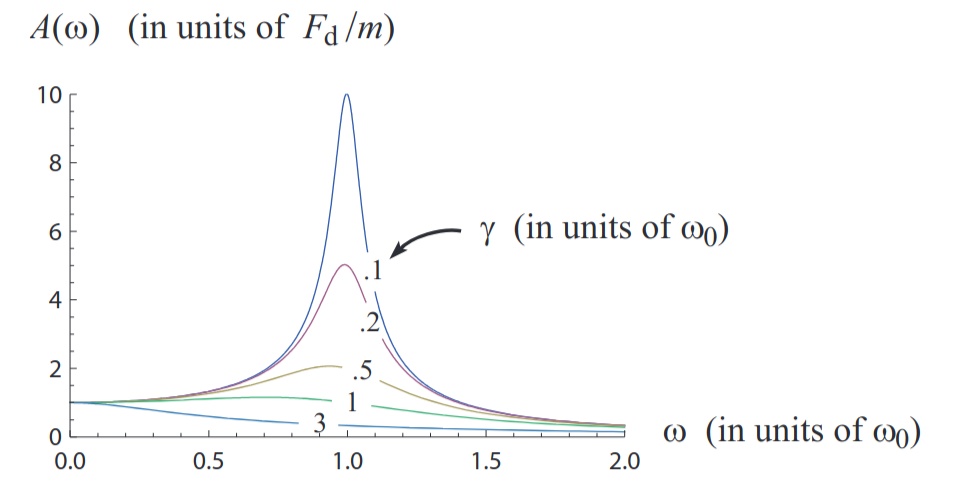
\includegraphics[width=\linewidth]{resonance_amplitude.png}
  }
  \hfill
  \subcaptionbox*{}[.48\linewidth]{
    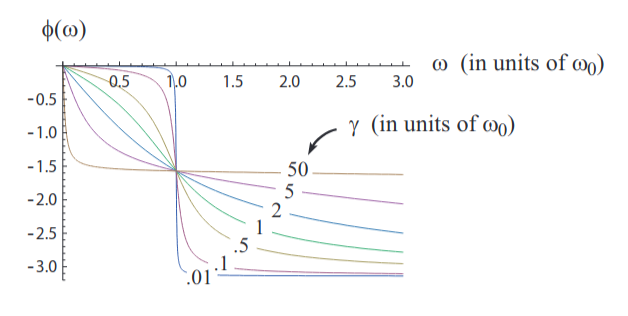
\includegraphics[width=\linewidth]{resonance_phase.png}
  }
\end{figure}

To help interpret the amplitude graph, we will introduce a new quantity: the \textbf{full width at half maximum} (FWHM; denoted by $\Gamma$). If we denote the maximum amplitude as $A_\text{peak}$, then $\Gamma$ describes the difference between the two $\omega$ values where $A = A_\text{peak}/2$. 

Assuming that $\gamma \ll \omega_0$, we have $A_\text{peak}/2 = F_d/(2\gamma m\omega_0)$. Then, if we say $\omega_{1/2}$ is the frequency where $A=A_\text{peak}/2$, 
\begin{align*}
    \frac{F_d}{2m\gamma\omega_0} &= \frac{F_d}{m}\frac{1}{\sqrt{(\omega_0^2-\omega_{1/2}^2)^2+(\gamma\omega_{1/2})^2}} \\
    4\gamma^2\omega_0^2 &= (\omega_0^2-\omega_{1/2}^2)^2+(\gamma\omega_{1/2})^2 \\
    \intertext{We can use the approximation $\omega_{1/2} \approx \omega_0$ on the $\gamma\omega_{1/2}$ term but \textbf{not} on the $\omega_0^2-\omega_{1/2}^2$ term (because the difference is so small, slight variations have a large impact). Thus,}
    4\gamma^2\omega_0^2 &\approx  (\omega_0^2-\omega_{1/2}^2)^2 + \gamma^2\omega_0^2  
\end{align*}
Or, rearranging slightly,
\begin{align*}
    (\omega_0^2-\omega_{1/2}^2)^2 &= 3\gamma^2\omega_0^2 \\
    \omega_{1/2}^2 &= \omega_0^2\pm \sqrt{3}\gamma\omega_0 \\
    \omega_{1/2} &= \omega_0\sqrt{1 \pm \sqrt{3}\frac{\gamma}{\omega_0}}
\end{align*}
Taylor expanding the square root term, we get $\sqrt{1\pm\sqrt{3}\gamma/\omega_0} \approx 1\pm \frac{\sqrt 3\gamma}{2\omega_0}$, so
\[ \omega_{1/2} = \omega_0 \pm \frac{\sqrt{3}}{2}\gamma\]
Then, the difference between the two $\omega_{1/2}$s is given by $\Gamma = \sqrt{3}\gamma$.

\section{Power}
In a driven and damped oscillator, the driving force feeds energy into the system at some points and takes energy out at others (except in the special case of resonance, where it always feeds energy in). The damping force always takes energy out. For the steady-state solution, the motion is periodic and so on average, the energy should remain constant. 

This means that the sum of the average powers from the driving force and the damping force over a complete oscillation should be zero.

For the following sections, assume the effect from the transient solution is negligible.
\subsection*{Power From the Damping Force}
Recall that the instantaneous power on an object from a force $F$ is $P =  Fv$. Therefore, 
\begin{align*}
    P_\text{damping} &= F_\text{damping}\dot x = -b\dot x^2  \\
    &= -b(-\omega A\sin(\omega t+\phi))^2 \\
    &= -b(\omega A)^2\sin^2(\omega t+\phi)
\end{align*}
The average power over a complete cycle is given by
\begin{align*}
    \langle P_\text{damping}\rangle &= \frac{1}{T}\int_0^T P_\text{damping}\dd t \\
    &= -b(\omega A)^2\pqty{\frac{1}{T}\int_0^T \sin^2(\omega t+\phi)\dd t} \\
    &= -\frac{1}{2}b(\omega A)^2
\end{align*}
Where the final equality comes from the fact that $\sin^2 \theta$, when integrated over a cycle, has an average value of $1/2$. 
\subsection*{Power From the Driving Force}
The instantaneous power from the driving force is
\begin{align*}
    P_\text{driving} &= F_\text{driving}\dot x = F_dA\cos(\omega t)\dot x \\
    &= -\omega F_dA\cos(\omega t)\sin(\omega t+\phi) \\
    &= -\omega F_dA\cos(\omega t)\pqty{\sin(\omega t)\cos(\phi) + \cos(\omega t)\sin(\phi)} \\
    &= -\omega F_dA\pqty{\cos(\phi)\sin(\omega t)\cos(\omega t) + \sin(\phi)\cos^2(\omega t)}
\end{align*}
The average value of the $\sin(\omega t)\cos(\omega t)$ term over a cycle is zero, and the average value of the $\cos^2(\omega t)$ term over a cycle is $1/2$, so
\[ \langle P_\text{driving} \rangle = -\frac{1}{2}F_dA\omega\sin\phi \]
We can rewrite $\sin\phi = -\gamma \omega mA/F_d$ (this is given without proof) to find
\[ \langle P_\text{driving}\rangle = \frac{1}2b(A\omega)^2\]
Therefore, we find $\langle P_\text{driving}\rangle + \langle P_\text{damping}\rangle = 0$, as expected. 

We will now turn our attention to $\langle P_\text{driving}\rangle$ on its own. If we plug in for $A$, we find that
\begin{align*}
    \langle P_\text{driving}\rangle &= \frac{1}{2}b\omega^2 \pqty{\frac{F_d}{m}\frac{1}{\sqrt{(\omega_0^2-\omega^2)^2+(\gamma\omega)^2}}}^2 \\
    &= \frac{\gamma mF_d^2}{2\gamma^2m^2}\frac{\gamma^2\omega^2}{(\omega_0^2-\omega^2)^2+(\gamma\omega)^2} \\
    &= \frac{F_d^2}{2\gamma m}\frac{\gamma^2\omega^2}{(\omega_0^2-\omega^2)^2+(\gamma\omega)^2}
\end{align*}
If we rewrite this as $\langle P_\text{driving}\rangle = (F_d^2/(2\gamma m)) f(\omega)$, we can plot the dimensionless quantity $f$ as a function of $\omega$. We may also plot the quantity $f/\gamma$ to see the actual average power, including the adjustment from $\gamma$.
\begin{figure}[t!]
  \subcaptionbox*{}[.48\linewidth]{
    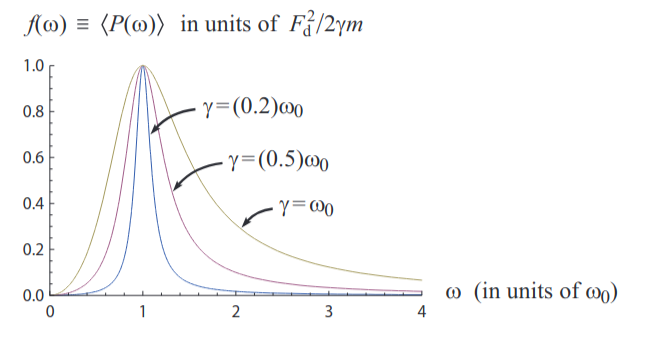
\includegraphics[width=\linewidth]{resonance_average_power_normed.png}
  }
  \hfill
  \subcaptionbox*{}[.48\linewidth]{
    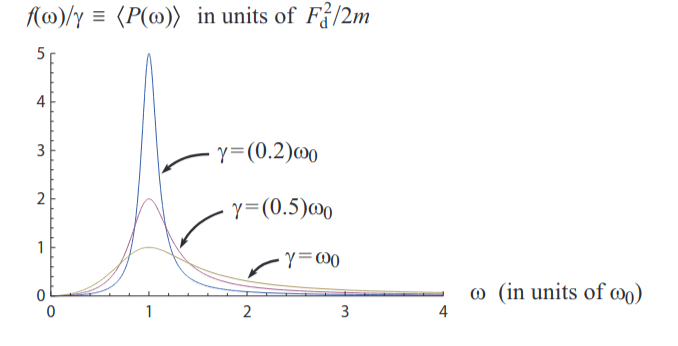
\includegraphics[width=\linewidth]{resonance_average_power_unnormed.png}
  }
\end{figure}
To find the maximum value of $f(\omega)$, we set its derivative equal to zero:
\begin{align*}
    \dv{f}{\omega} &= \frac{[(\omega_0^2-\omega^2)^2+(\gamma\omega)^2][2\gamma^2\omega] - [\gamma^2\omega^2][-4\omega(\omega_0^2-\omega^2)+2\gamma^2\omega]}{[(\omega_0-\omega^2)^2 + (\gamma\omega)^2]^2} 
\end{align*}
The denominator is never zero, so we can just set the numerator equal to zero,
\begin{align*}
    [\gamma^2\omega^2][-4\omega(\omega_0^2-\omega^2)+2\gamma^2\omega] &= [(\omega_0^2-\omega^2)^2+(\gamma\omega)^2][2\gamma^2\omega] \\
    -2\omega^2(\omega_0^2-\omega^2)+\gamma^2\omega^2 &= (\omega_0^2-\omega^2)^2 +(\gamma\omega)^2 \\
    (\omega_0^2-\omega^2)(\omega_0^2+3\omega^2) &= 0
\end{align*}
Therefore, the maximum is achieved at $\omega=\omega_0$. We also find that the maximum value of $f(\omega)$ is equal to one, so to find $\Gamma$ we set it equal to $1/2$. This means that
\[ \frac{\gamma^2\omega^2}{(\omega_0^2-\omega^2)^2+(\gamma\omega)^2} = \frac{1}{2}\]
implying that $\omega_0^2-\omega^2 = \pm \gamma\omega$. If we let $\omega_1$ be the solution given by $\omega_0^2-\omega_1^2 = \gamma\omega_1$ and $\omega_2$ be the solution given by $\omega_0^2-\omega_2^2= -\gamma\omega_w$, we take the difference to find
\begin{align*}
    \omega_2^2 - \omega_1^2 = \gamma(\omega_2+\omega_1) \implies \omega_2-\omega_1 = \gamma
\end{align*}
Therefore, the FWHM of this curve is given by $\Gamma = \gamma$. This is a nice result, and unlike the previous resonance results, holds in its exactness no matter the size of $\gamma$ (as we used no approximations to get here).

% \begin{align*}
%     \omega^2 &= \frac{2\omega_0^2+\gamma\pm \sqrt{(2\omega_0^2+\gamma^2)^2-4(\omega_0^4-4\gamma^2\omega_0^2)}}{2} \\
%     &= \omega_0^2 + \frac{\gamma^2}{2} \pm \frac{1}{2}\sqrt{4\omega_0^4+4\omega_0^2\gamma^2+\gamma^4 - 4\omega_0^4 + 16\gamma^2\omega_0^2} \\
%     &= \omega_\text{resonance}^2 \pm \frac{1}2\sqrt{20\omega_0^2\gamma^2 + \gamma^4} \\
%     &= \omega_\text{resonance}^2 \pm \frac{\gamma}{2}\sqrt{20\omega_0^2+\gamma^2}
% \end{align*}



% Consider a mass $m$ attached to a spring with spring constant $k$ that is undergoing a damping force with coefficient $b$. Now, suppose the mass has some periodic external force $F=F_D\cos\omega t$. Then, the equation of motion is given by
% \[ m\ddot x +b\dot x+k x = F_D\cos\omega t\]
% We will also write $\tilde F = F_De^{i\omega t}$, so $F_D\cos\omega t = \Re \tilde F$. We will rephrase our differential equation as
% \[ m\ddot x + b\dot x +k x = F_De^{i\omega t} \]
% Although this is slightly different, it turns out we can just take the real part at the end. Now, we guess a solution of the form
% \[ x(t) = Ae^{i(\omega t+\phi)} \]
% Notice that we have just claimed that the frequency of the motion is  the same as the frequency of the driven oscillator. In reality, there are two parts of a solution: the \textbf{transient solution}, which is determined by the initial conditions (and dies down to zero as $t$ increases; the transient solution is the solution to the homogeneous equivalent of our equation of motion), and the \textbf{steady-state solution}, which is determined by the driving force, and will persist. We claim that the frequency of the steady-state solution is the same as the frequency of the driving force
% \[ \Re x(t) = |A|\cos(\omega t+\phi)\]
% plugging this in to our differential equation,
% \[ Ae^{i\omega t}(-m\omega^2 + ib\omega + k) = F_De^{i\omega t} \]
% where $A = |A|e^{i\phi}$. Now, we can solve for $A$ to obtain
% \begin{align*}
%     A &= \frac{F_D}{-m\omega^2-ib\omega+k} \\
%     &= \frac{F_D}{m}\pqty{\frac{1}{-\omega^2+i\omega(b/m) + (k/m)}} \\
%     &= \frac{F_D}{m}\pqty{\frac{1}{(\omega_0^2-\omega^2) + i\omega\gamma}}
% \end{align*}
% We wish to remove the complex part from the denominator, so we multiply the numerator and denominator by $(\omega_0^2-\omega^2)-i\omega\gamma)$ to obtain
% \begin{align*}
% A &= \frac{F_D}{m}\pqty{\frac{(\omega_0^2-\omega^2)-i\omega\gamma}{(\omega_0^2-\omega^2)^2+\omega^2\gamma^2}}
% \end{align*}
% The magnitude of $A$ is then
% \begin{align*}
%     |A|^2 = AA^* &= \pqty{\frac{F_D}{m}}^2\pqty{\frac{(\omega_0^2-\omega^2)^2+\omega^2\gamma^2}{[(\omega_0^2-\omega^2)^2+\omega^2\gamma^2]^2}}\\
%     &= \pqty{\frac{F_D}{m}}^2\pqty{\frac{1}{(\omega_0^2-\omega^2)^2+(\omega\gamma)^2}}
% \end{align*}
% So
% \[ |A| = \frac{F_D}{m}\frac{1}{\sqrt{(\omega_0-\omega)^2+(\gamma\omega)^2}}\]
% To find the phase of $A$, we note that $\tan\phi = \Im A/\Re A$, so
% \begin{align*}
    % \tan\phi &= \frac{-\omega \gamma}{\omega_0^2-\omega^2}
% \end{align*}
% we may also use $\sin\phi = -\omega\gamma m|A|/F_D$.

% One important result is that $\phi$ is always negative--this means that the position is always lagging behind the force, which makes sense with our concept of acceleration. Further, as $\omega\to 0$, $\phi\to 0$ and as $\omega\to\infty$, $\phi\to -\pi$.

% As $\omega\to 0$, we have $|A|\to F_D/k$, so $F_D\to k|A|$. This means that the driving force balances the restoring force; $F_D + F_s = k|A| - kx$ and the system approaches a steady state. 

% Consider the power given to the system by the driving force. It is given by $P=F\dot x = F_D\cos(\omega t) \dot x$, so
% \[ P = -F_D\omega |A|\cos\omega t\sin\omega t\]
% (the $+\phi$ goes away because $\omega$ is small and so $\phi\to 0$). Then, the total work done in a period is $\int_0^T P\dd t = 0$, because the sinusoidal terms cancel each other out. Thus, on average, the driving force does no work on the system.

% When $\omega$ is very large, a very similar argument can be used to find that the driving force does very little work.

% Now, we will consider what happens when $\omega = \omega_0$. The amplitude becomes
% \[ |A| = \frac{F_D}{m}\frac{1}{\omega\gamma}\]
% We can rewrite this as
% \begin{align*}
%     |A| &= \frac{F_D}{m\omega_0^2}\frac{\omega_0}{\gamma} = \frac{F_D}{m(k/m)}\frac{\omega_0}{\gamma} \\
%     &= \frac{F_D}{k}\frac{\omega_0}{\gamma} = \frac{F_D}{k}Q
% \end{align*}
% This essentially means that if $Q$ is larger, we can get a higher resonant amplitude much easier. 

% We can additionally find that $\dd |A|^2/\dd \omega = 0$ when $\omega= \sqrt{\omega_0^2-\gamma^2/2}\approx \omega_0$ (small $\gamma$). Therefore, the amplitude is at its maximum when $\omega\approx \omega_0$.

% And the phase becomes $\phi = -\pi/2$ because $\tan\phi\to\pm \infty$. This is how we discoverer resonances in nature; by looking for a simultaneous amplitude peak and a 90 degree phase shift.

% Computing the power in this scenario, we have
% \begin{align*}
%     P = Fv &= F_D\cos(\omega t)\cdot |A|\omega \sin(\omega t +\pi/2) \\
%     &= F_D\omega|A|\cos^2(\omega t)
% \end{align*}
% This arises because the driving force and velocity are exactly in phase at the resonance, and therefore obtain peak amplitude.

% The resonant frequency is where the most efficient delivery of energy occurs. 

% We also wish to study the dissipative force at the resonant amplitude. Recall that when in resonance, 
% \[ x_s(t) = |A_s|\cos(\omega_0 t - \pi/2) = |A_s|\sin(\omega_0 t)\]
% so $v_s(t) = -|A_s|\omega_0\cos(\omega_0 t)$. Plugging this into $F_\text{drag} = -bv$, we have
% \[ F_\text{drag} = -b|A_s|\omega_0\cos(\omega_0t) = -\frac{bF_D\omega_0}{m\omega_0\gamma}\cos(\omega_0t) = -F_D\cos(\omega_0t)\]
% This essentially tells us that at the peak of the resonance, the driving force and resistant force cancel each other out.

% We will define a new quantity known as the \textbf{full width half maximum} (FWHM), denoted by $\Gamma$, which tells us the distance between the two points on a graph of $|A|$ vs $\omega$ where $|A| = |A|_\text{peak}/2$. In other words, it is the distance between $\omega_1$ and $\omega_2$ where
% \[ |A|_{\omega_1} = |A|_{\omega_2} = \frac{F_D}{2m}\frac{1}{\gamma\omega}\]
% Therefore, if $\omega'$ is either $\omega_1$ or $\omega_2$,
% \begin{align*}
%     \frac{F_D}{m}\frac{1}{\sqrt{(\omega_0^2-\omega'^2)^2+(\gamma\omega')^2}} &= \frac{F_D}{m}\frac{1}{2\gamma\omega} \\
%     (\omega_0^2-\omega'^2)^2 + (\gamma\omega')^2 &= 4\gamma^2\omega_0^2 \\
%     \omega'^4 - (2\omega_0^2+\gamma^2)\omega'^2 + \omega_0^4(1-4\gamma^2) &= 0
% \end{align*}
% So FWHM $ = \sqrt{3} \gamma$.

% \subsection*{Including the Transient Solution}
% Previously, we made the claim that the steady solution dominates as $t\to\infty$. Now, we justify that claim.

% First, suppose the transient solution is $x_\text{tr}(t)$ and the steady solution is $x_\text{s}(t)$. The most general form of $x(t)$ is
% \begin{align*}
%     x(t) &= x_\text{tr} + x_\text{s} \\
%     &= |A_\text{tr}|e^{-\gamma t/2}\cos(\omega't+\phi') + |A_\text{s}|\cos(\omega t + \phi)
% \end{align*}
% With the initial condition $x(0)=0$ and $x'(0)=0$, we have $\phi' = -\pi/2$ and $|A_\text{tr}| = |A_\text{s}|$. Additionally, for small $\gamma$ we have $\omega' \approx \omega_0$, and at resonance $\omega \approx \omega_0$. Then, $x(t)$ becomes
% \[ x(t) = |A_\text{s}|(1-e^{-\gamma t/2})\sin(\omega t)\]
% So as $t$ increases, $x(t)\to x_\text{s}(t)$. The amount of time it takes for the transient solution to die down is proportional to $\tau = 1/\gamma$. 
% \subsection*{Power Delivery (General Frequency)}
% Assuming the transient solution is sufficiently small, the instantaneous power from the driving force is given by $P_D = (F_D\cos\omega t)(-|A|\omega\sin(\omega  t + \phi))$. The average power over a period of oscillation is given by
% \begin{align*}
%     \langle P_D\rangle &= \frac{1}{T}\int_0^T P\dd t \\
%     &= -\frac{F_D\omega|A|}{T}\int_0^T \cos(\omega t)\sin(\omega t +\phi) \dd t \\ 
%     &= -\frac{F_D\omega|A|}{T}\int_0^T \cos(\omega t)\pqty{\sin\omega t \cos\phi + \cos\omega t\sin\phi} \dd t \\
%     &= -\frac{F_D\omega|A|\cos\phi}{T}\int_0^T \cos\omega t\sin\omega t \dd t - \frac{F_D\omega |A|\sin\phi}{T}\int_0^T \cos^2\omega t\dd t
%     \intertext{The left term goes to zero, so }
%     \langle P_D \rangle &= -\frac{F_D\omega|A|\sin\phi}{T}\int_0^T \cos^2\omega t \dd t \\
%     &= -\frac{F_D\omega |A|\sin\phi}{2} = -\frac{F_D\omega|A|(-\omega\gamma m|A|)}{2F_D} = \frac{1}{2}b\omega^2|A|^2 
% \end{align*}
% The instantaneous power from the dissipating force is given by $P_R = -bv^2 = -b\omega^2|A|^2\sin^2(\omega t+\phi)$. So the average power from the dissipating force over a period of oscillation is
% \begin{align*}
%     \langle P_R\rangle &= \frac{1}{T}\int_0^T -b\omega^2|A|^2\sin^2(\omega t+\phi)\dd t \\
%     &= -\frac{1}{2}b\omega^2|A|^2
% \end{align*}
% So the total average power over an oscillation is $\langle P\rangle = \langle P_R\rangle + \langle P_D\rangle = 0$. This means that the energy of a steady driven harmonic oscillator is constant. Also note that these results apply at any frequency, not just in resonance. 

% Although the driving power will always cancel with the resistive power, the magnitude of the power input into the system (by the driving force) is given by
% \begin{align*}
%     \langle P_D\rangle &= \frac{F_D^2}{2m\gamma}\frac{\gamma^2\omega^2}{(\omega_0^2-\omega^2)^2+(\gamma\omega)^2} 
% \end{align*}
% which tells us that the power peaks at the resonance $\omega=\omega_0$, with a value of
% \[ \langle P_D\rangle_\text{max} = \frac{F_D^2}{2m\gamma} \]
% We also find that the FWHM of this curve is exactly $\Gamma = \gamma$. Therefore, we have $\Gamma\tau = 1$, which is one of the critical universal properties of resonant motion. 
 % regular oscillations
\chapter{Coupled Oscillations; Normal Modes}
Consider a system of two masses, with each connected to a fixed wall by a spring of constant $k$, and the two masses are connected to each other by a spring of spring constant $k'$. 

If we define $x_1$ and $x_2$ as the positions of the masses, where $x_1=0$ denotes the equilibrium position of the first mass and $x_2=0$ denotes the equilibrium position of the second mass.

The equations of motion become
\[ m\ddot x_1 = -kx_1 - k'(x_1-x_2)\]
\[ m\ddot x_2 = -kx_2 -k'(x_2-x_1)\]
\subsection*{Energy}
Analyzing the energy of the system, we see
\begin{align*}
    U &= \frac{1}{2}kx_1^2 + \frac{1}{2}k'(x_1-x_2)^2 + \frac{1}{2}kx_2^2  
\end{align*}
So we can derive the forces on either mass with $F_1 = -\partial U/\partial x_1$ and $F_2 = -\partial U/\partial x_2$. 

\subsection*{Coupled Pendulums}
Consider two pendulums each with length $\ell$ and a mass $m$ suspended from them, connected by a spring with spring constant $k$. We will consider the energy of these pendulums.

The potential energy from the height of $m_1$ is given by 
\[ U_1 = mg\ell(1-\cos\theta) \approx \frac{1}{2}mg\ell\theta^2 = \frac{1}{2\ell}mgx_1^2 \]
where $x_1$ is the arclength traveled by $m_1$ away from equilibrium. The potential energy from $m_2$ is given similarly, and the potential energy from the spring is given by $\frac{1}2 k(x_1-x_2)^2$, so
\[ U = \frac{1}{2\ell}mgx_1^2 + \frac{1}{2\ell}mgx_2^2 + \frac{1}{2}k(x_1-x_2)^2\]
which tells us
\begin{align*}
    F_1 = -\pdv{U}{x_1} &= -\frac{mg}{\ell}x_1 - k(x_1-x_2) \\
    F_2 = -\pdv{U}{x_2} &= -\frac{mg}{\ell}x_2 - k(x_2-x_1)
\end{align*}

\section{Solution to the Equation of Motion}
We will focus on the first scenario, with the masses coupled by three springs. But the same analysis applies quite readily to the pendulum case, and indeed to many other analogous cases.
\subsection*{First Method}
The first method is the easiest but is only applicable to a small subset of problems. If we add the equations of motion for $x_1$ and $x_2$ together, we see
\[ m(\ddot x_1 + \ddot x_2) = -k(x_1+x_2)\]
Then, subtracting the second equation from the first yields
\[ m(\ddot x_1 - \ddot x_2) = (-k+2k')(x_1-x_2)\]
If we define the two quantities $\omega_s = \sqrt{k/m}$ (slow frequency) and $\omega_f = \sqrt{(k+2k')/m}$ (fast frequency), we get the two solutions
\begin{align*}
    x_1(t) + x_2(t) &= 2A_s\cos(\omega_s t + \phi_s) \\
    x_1(t) - x_2(t) &= 2A_f\cos(\omega_f t+\phi_f)
\end{align*}
The reason for the twos in front of the amplitudes will become clear momentarily. The critical result here is that there are two \textit{modes} of oscillation--one for $x_1+x_2$ and one for $x_1-x_2$. 

To pick out either $x_1$ or $x_2$, we can subtract or add the two equations to find
\begin{align*}
    x_1(t) &= A_s\cos(\omega_st+\phi_s) + A_f\cos(\omega_ft+\phi_f) \\
    x_2(t) &= A_s\cos(\omega_st+\phi_s)-A_f\cos(\omega_ft+\phi_f)
\end{align*}
Now, suppose we impose the four initial conditions $x_1(0)=0$, $\dot x_1(0)=0$, $x_2(0)=A$, and $\dot x_2(0)=0$. We can get expressions for $\dot x_1$ and $\dot x_2$,
\begin{align*}
    \dot x_1(t) &= -A_s\omega_s\sin(\omega_s t+\phi_s) - A_f\omega_f\sin(\omega_ft+\phi_f) \\
    \dot x_2(t) &= -A_s\omega_s\sin(\omega_s t+\phi_s) + A_f\omega_f\sin(\omega_ft+\phi_f)
\end{align*}
This means that
\begin{align*}
    0 &= A_s\cos\phi_s + A_f\cos \phi_f \\
    0&= -A_s\omega_s\sin\phi_s -A_f\omega_f\sin\phi_f \\
    A &= A_s\cos\phi_s - A_f\cos\phi_f \\
    0 &= -A_s\omega_s\sin\phi_s + A_f\omega_f\sin\phi_f
\end{align*}
Adding equations (1) and (3) and (2) and (4) yields
\begin{align*}
    2A_s\cos\phi_s &= A \\
    2A_s\omega_s\sin\phi_s &= 0
\end{align*}
So $\phi_s = 0$, $A_s=A/2$. Then, subtracting (3) from (1) and (2) from (4) gives
\begin{align*}
    2A_f\cos\phi_f &= -A \\
    2A_f\omega_f\sin\phi_f &= 0
\end{align*}
So $A_f = -A/2$ and $\phi_f = 0$. Then, $x_1$ and $x_2$ are
\begin{align*}
    x_1(t) &= \frac{A}{2}(\cos\omega_s t - \cos \omega_f t) = A\sin\pqty{\frac{(\omega_f-\omega_s)t}{2}}\sin\pqty{\frac{(\omega_f+\omega_s)t}{2}} \\
    x_2(t) &= \frac{A}{2}(\cos \omega_s t + \cos\omega_f t)= A\cos\pqty{\frac{(\omega_f-\omega_s)t}{2}}\cos\pqty{\frac{(\omega_f+\omega_s)t}{2}}
\end{align*}
Defining $\Omega \equiv (\omega_f+\omega_s)/2$ and $\epsilon\equiv (\omega_f-\omega_s)/2$, we note that $\Omega$ will be much larger than $\epsilon$, so the equations of motion
\begin{align*}
    x_1(t) &= A\sin\Omega t\sin\epsilon t \\
    x_2(t) &= A\cos\Omega t\cos\epsilon t
\end{align*}
produce a phenomenon known as \textbf{beat waves}; the slow $\epsilon$ oscillator determines the amplitude of the fast $\Omega$ waves.

In the special case where $x_1$ and $x_2$ are perfectly in phase or perfectly out of phase, the quantity $x_1-x_2$ in the original differential equation of motion is completely constant and so the differential equation reduces to
\[ m\ddot x_1 = -kx_1 - k'\delta \]
\[ m\ddot x_2 = -kx_2 + k'\delta \]
where $\delta \equiv x_1-x_2$ is constant. Then, the differential equations become entirely uncoupled and act like regular harmonic oscillators. 
\subsection*{Second Method}
We will now explore a different, more general way of solving the coupled differential equations. First, we will rephrase our problem using a matrix. The differential equation
\begin{align*}
    m\ddot x_1 &=-kx_1 -k'(x_1-x_2) \\
    m\ddot x_2 &= -kx_2 - k'(x_2-x_1)
\end{align*}
Defining the position vector $\mbf x = \begin{pmatrix}
    x_1(t) \\ x_2(t)
\end{pmatrix}$, the mass matrix $\mbf M = \begin{pmatrix}
    m & 0 \\
    0 & m
\end{pmatrix}$, and the spring constant matrix $\mbf K = \begin{pmatrix}
    k+k'  & -k' \\
    -k' & k+k'
\end{pmatrix}$ the differential equation can be rephrased:
\begin{align*}
    \mbf M \mbf{\ddot x} &= -\mbf K \mbf x
\end{align*}
We can guess the fictitious complex solution (which we will take the real component of later) $\mbf z = \mbf a e^{i\omega t}$ where $\mbf a\in\C^2$ is a constant vector. Then, the differential equation becomes
\[ -\mbf M \omega^2 \mbf a e^{i\omega t} = -\mbf K\mbf a e^{i\omega t}\]
Or, in other words,
\[ (\mbf K -\omega^2 \mbf M)\mbf a = 0\]
This has either only the trivial solution $\mbf a =\mbf 0$ if $\mbf K - \omega^2\mbf M$ is invertible, or a set of solutions if $\mbf K -\omega^2\mbf M$ is not invertible. We are only interested in the nontrivial case, so we want to ensure $\det(\mbf K -\omega^2\mbf M) = 0$. This gives
\begin{align*}
    \det \begin{pmatrix}
        k+k'-m\omega ^2 & -k' \\
        -k' & k+k'-m\omega^2
    \end{pmatrix} = (k+k'-m\omega^2)^2 + (k')^2 = 0
\end{align*}
The solutions to this equation give exactly the normal frequencies of the system. 
\section{Normal Modes}
Before, we found two \textit{normal frequencies} $\omega_s = \sqrt{k/m}$ and $\omega_f = \sqrt{(k+2k')/m}$. Each of these frequencies correspond to a perfectly sinusoidal motion for each mass.

To see this, consider the case where $x_1$ and $x_2$ oscillate perfectly in phase with one another, so $x_1=x_2$ and
\begin{align*}
    m\ddot x_1 &= -kx_1 - k'(x_1-x_2) = -kx_1\\
    m\ddot x_2 &= -kx_2 + k'(x_1-x_2) = -kx_2
\end{align*}
So the oscillations have frequency $\sqrt{k/m}$, which is just the slow frequency $\omega_s$.

Now, let $x_1$ and $x_2$ oscillate perfectly out of phase with one another, so
\begin{align*}
    m\ddot x_1 &= -kx_1-k'(x_1-x_2) = -(k+2k')x_1 \\
    m\ddot x_2 &= -kx_2 + k'(x_1-x_2) = -(k+2k')x_2
\end{align*}
So the oscillations have frequency $\sqrt{(k+2k')/m}$, which is just the fast frequency $\omega_f$.
\section{N Masses}
Consider a string of tension $T$ with $N$ masses $m_1, m_2, \dots, m_N$ threaded on it, each mass separated by a distance $a$.

The force in the $y$ direction for mass $n$ can be written as
\[ m\ddot x_n= -T\sin\theta_{n} - T\sin\theta_{n-1}\]
or
\begin{align*}
    m\ddot x_n &= -T(\sin\theta_n + \sin\theta_{n+1}) \\
    &= -T\pqty{\frac{x_n-x_{n-1}}{a} + \frac{x_{n}-x_{n+1}}{a}} \\
    &= \frac{T}{a}(x_{n-1}-2x_n + x_{n+1})
\end{align*}
Guessing a solution $y_n(t) = A_ne^{i\omega t}$, we find
\begin{align*}
    -A_nm\omega^2 &= \frac{T}{a}(A_{n-1}-2A_n+A_{n+1})
\end{align*}
or
\[ -A_{n-1} + \pqty{2-\frac{m\omega^2 a}{T}}A_n - A_{n+1} = 0\]
This allows us to write
\[ \frac{A_{n-1}+A_{n+1}}{A_n} = \frac{2\omega_0^2-\omega^2}{\omega_0^2}\]
where we define $\omega_0^2 = (T/a)(1/m)$. Remarkably, this means that the ratio $(A_{n-1}+A_{n+1})/A_n$ is constant regardless of the value of $n$.

Generally, the coefficients $A_n$ are complex, so we write them as $A_r = |C|e^{i\delta}e^{i\theta_n}$. The phase $\delta$ represents the phase of the \textit{whole system}, while $\theta_n$ represents the phase of just the mass $n$.

We additionally make the assumption that each $\theta_n = n\theta$ for a fixed $\theta$. We will see why this works later. 

Plugging this into the ratio,
\begin{align*}
    \frac{e^{i(n-1)\theta}+e^{i(n+1)\theta}}{e^{in\theta}}  &= e^{-i\theta}+e^{i\theta} = 2\cos\theta 
\end{align*}
so, $2\cos\theta = (2\omega_0^2-\omega^2)/\omega_0^2$.

Next, we will consider the idea of \textbf{boundary conditions}. Since the ends of the string are fixed at $y=0$, we have $\Re A_0 = \Re A_{N+1} = 0$. Thus
\[ \Re A_0  = \Re |C|e^{i\delta}e^{0} = \Re |C|e^{i\delta} = |C|\cos(\delta) \]
Since $|C|=0$ implies no motion, we are not interested in that solution. So we have $\delta = \pm \pi/2$. We will arbitrarily choose to use $-\pi/2$, so
\begin{align*}
    A_n = |C|e^{-i\pi/2}e^{in\theta}
\end{align*}
So we also have
\[ \Re A_{N+1} = \Re |C|e^{i\delta}e^{i(N+1)\theta} = |C|\cos((N+1)\theta+\delta)\]
Since $\delta=-\pi/2$, we must then have $(N+1)\theta = m\pi$ for some $m$. Thus, 
\[ \theta = \frac{m\pi}{N+1}\]
Where $m = 1, 2, \dots, N$. The reason $m$ stops at $N$ is because each $m$ represents a normal mode; since  there are $N$ normal modes, we look for $N$ unique $\theta$s. If we considered $m>N$, we would notice that the values of $m$ begin to repeat themselves and give no new information.

We also know that $2\cos(\theta) = (2\omega_0^2-\omega^2)/\omega_0^2$, so
\[ \omega_m = 2\omega_0\sin\pqty{\frac{m\pi}{2(m+1)}}\]
This means that for mass $n$ in normal mode $m$ at time $t$,
\[ y_n^m(t) = |C|e^{-\pi/2}e^{inm\pi/(N+1)}e^{i\omega_m t} = |C|e^{i\omega_m t + in\theta - \pi/2}\]
so
\[ \Re y_n^m(t) = \sin(\omega_m t + n\theta )\]
Because of how we defined $\omega_m$, we see that $2\omega_0$ is the largest possible normal mode frequency in the system (cutoff frequency). We may also write
\[ \omega_0 = \sqrt{\frac{T}{ma}} = \frac{1}{a} \sqrt{\frac{T}{m/a}} = \frac{1}{a}\sqrt{\frac{T}{\mu}}\]
where we defined $\mu\equiv m/a$ as the linear mass density.

\subsection*{$N\to\infty$}
Letting $N\to\infty$, we can rephrase our $y_r$s as a function of a continuous position $x$, giving an equation of motion 
\begin{align*}
    m\pdv[2]{y}{x} &= \frac{T}{m}\pqty{\frac{y(x+\Delta x)-y(x)}{\Delta x} + \frac{y(x)-y(x-\Delta x)}{\Delta x}} \\
    &= \frac{T}{m}\pqty{y_x(x) + y_x(x-\Delta x)} \\
    &= \Delta x\frac{T}{m} \pdv[2]{y}{x} \\
    \frac{m}{\Delta x} \pdv[2]{y}{t} &= T\pdv[2]{y}{x} \\
    \mu\pdv[2]{y}{t} &= T\pdv[2]{y}{x}
\end{align*}
This is the \textbf{wave equation}. We can note that the quantity $\sqrt{T/\mu}$ has units of velocity, so we can define the velocity of the wave as $c^2\equiv T/\mu $, and write
\[ \pdv[2]{y}{t} = c^2\pdv[2]{y}{x} \]
 % coupled oscillations and normal modes
\chapter{Transverse Waves}
In the previous chapters, we built the foundation necessary to begin studying waves. We will first consider non-dispersive waves, which have the special property that all waves travel with the same speed, regardless of their wavelength and frequency. Later, we will explore dispersive waves, which change speed depending on their wavelength and frequency.


There are two types of waves: transverse and longitudinal waves. Transverse waves have a disturbance normal to the direction of propagation (this is the type of wave we analyzed previously). Longitudinal waves have a disturbance along the direction of propagation.
\section{The Wave Equation}
Consider a string with a constant tension $T$ applied to it, connected to two walls on either side at the same height.  

If a pulse is applied to the system at some point along the string, we expect the pulse to travel through the string until it reaches the far end, upon which it will reflect. For a small deformed section of the string, there are two tension forces, pointing nearly in opposite directions. These tension forces will have a longitudinal component and a transverse component. The longitudinal components cancel and each tension has a transverse component
\[ T\sin\theta \quad\text{and}\quad T\sin(\theta+\dd\theta)\]
for small angles, we write $\sin\theta\approx \tan\theta$, $\sin(\theta+\dd\theta) \approx \tan(\theta+\dd\theta)$. If the transverse component of the wave is described by a function $\psi(x,t)$ called the \textbf{wavefunction}, we can write $\tan\theta = \partial \psi/\partial x$. So, the total restoring force (pointing downwards) is given by
\[ F = T\pdv{\psi(x+\dd x, t)}{x}-T\pdv{\psi(x, t)}{x} = T\pdv[2]{\psi(x,t)}{x}\dd x\]
The mass of the small section of string is given by $m = \mu\dd x$ (technically, it is given by $\mu\sqrt{\dd x^2+\dd\phi^2}$, but we assume oscillations are small so $\sqrt{\dd x^2+\dd\phi^2}\approx \dd x$), so we find the equation of motion
\[ \pdv[2]{\psi}{x} = \frac{1}{c^2} \pdv[2]{\psi}{t}\]
where $c^2\equiv T/\mu$ is the speed of propagation of the wave (\textit{phase velocity}). This is the same wave equation we previously found.

We will guess a solution to this equation in the form $\psi(x,t) = a(x)e^{i\omega t}$. Then, we have
\[ \pdv[2]{\psi}{x} = \dv[2]{a}{x} e^{i\omega t}\quad\text{and}\quad \pdv[2]{\psi}{t} = -\omega^2 a(x)e^{i\omega t}\]
Thus, we wave equation becomes
\begin{align*}
    c^2\dv[2]{a}{x}e^{i\omega t} &= -\omega^2 a e^{i\omega t} \\
    \dv[2]{a}{x} &= -\frac{\omega^2}{c^2} a
\end{align*}
But this is just the regular harmonic oscillator, so we find that 
\[ a(x) = Ae^{\pm ikx} \]
where $k\equiv \omega/c$ is the \textbf{wave number}, and has units of $1/m$. 

But what is the physical interpretation of the wave number? If we denote the wavelength of $a$ with $\lambda$, the wave number is related to $\lambda$ with
\[ k = \frac{2\pi}{\lambda} \]
That is, $k$ is the number of radians of spatial oscillations in one unit length. The relationship between $k$ and $\lambda$ is analogous to the relationship between $\omega$ and $\nu$.

Plugging this back into our guess, we find that
\[ \psi(x,t) = Ae^{\pm ikx \pm i\omega t}\]
The most general solution is the sum of each of these four combinations,
\[ \psi(x,t) = Ae^{i(kx+\omega t)} + Be^{i(kx-\omega t)} + B^{*}e^{i(-kx+\omega t)} + A^{*}e^{i(-kx-\omega t)} \]
Where the conjugates appear from the requirement that $\psi(x,t)$ is real.

There are two main (equivalent) forms of this equation that will use, depending on the context.
\begin{enumerate}
    \item For a \textbf{traveling wave}, where one wave is moving to the left and one is moving to the right, we can write
    \[ \psi(x,t) = A_1\cos(kx + \omega t + \phi_1) + A_2\cos(kx - \omega t + \phi_2)\]
    \item For a \textbf{standing wave}, where all points on the string pass the $x$ axis at the same time, we can write
    \[ \psi(x,t) = A_1 \cos(kx+\phi_1)\cos(\omega t) + A_2\cos(kx+\phi_2)\sin(\omega t)\]
    We will revisit standing waves later.
\end{enumerate}
\subsection*{Traveling Waves}
Consider a traveling wave of the form
\[ \psi(x,t) = A_1\cos(kx + \omega t +\phi_1) \]
(we throw out the other term just for ease of visualization). At some $t$ value $t^*$, the wave looks like
\[ \psi(x, t^*) = A_1\cos(kx + \omega t^* + \phi_1) \]
This looks like a cosine graph with an ``effective phase" $\omega t^* + \phi_1$. Then, at some later time $t^* + \Delta t$, the graph looks the same, but shifted over to the left by some amount, giving a new effective phase of $\omega t^* + \omega \Delta t + \phi_1$. 

If $\Delta t=1$, we find that the horizontal shift is just $\omega/k$. Thus, we call the speed of the wave $c = \omega/k$. Visually, this looks like the wave is moving over as time passes, which is where the name "traveling wave" originates.
\subsection*{A more general solution}
But our assumed solution $\psi(x,t) = Ae^{i(\pm kx \pm \omega t)}$ is far from the most general solution to the wave equation
\[ \pdv[2]{\psi}{t} = c^2 \pdv[2]{\psi}{x} \]
Consider now the proposed solution $\psi(x,t) = f(x \pm ct)$. We can use the chain rule to determine
\[ \pdv[2]{\psi}{x} = \pdv[2]{f}{u} \quad\text{and} \quad \pdv[2]{\psi}{t} = c^2\pdv[2]{f}{u}\]
where $u = x\pm ct$. Thus, $\psi(x,t) = f(x \pm ct)$ solves the wave equation.

This can actually be connected with the solutions $a(x)e^{\pm i\omega t}$ with Fourier analysis, as we will cover later. For now though, we can just say that $\psi(x,t) = f(x\pm ct)$ is equivalent to saying
\[ \psi(x,t) = A_1\cos(k_1x)\cos(ck_1 t) + A_2\cos(k_2x)\cos(ck_2t) + \cdots \]
\section{Reflection and Transmission}
\subsection*{Applying the Boundary Conditions}
Instead of an infinite uniform string, consider an infinite string with density $\mu_1$ for $-\infty < x < 0$ and $\mu_2$ for $0 < x < \infty$. Although the density isn't uniform, the tension is still uniform throughout the whole string (otherwise it would be accelerating horizontally).

Assume that a traveling wave of the form $\psi_i(x,t) = f_i(x - c_1t)$ starts off at the far right and moves towards $x=0$. We may equivalently write $\psi_i(x,t) = f_i\pqty{t - \frac{x}{c_1}}$, which turns out to be much more convenient in this case. As this so-called \textbf{incident wave} approaches $x=0$, what happens to it? 

The most general thing that can happen is that there is some \textbf{reflected wave}
\[ \psi_r(x,t) = f_r\pqty{t + \frac{x}{c_1}}\]
and some \textbf{transmitted wave}
\[ \psi_t(x,t) = f_t\pqty{t - \frac{x}{c_2}}\]
In terms of the reflected and transmitted waves, the total expressions for the waves on the left and right are, respectively,
\begin{align*}
   \psi_L(x,t) &= \psi_i(x,t) + \psi_r(x,t) = f_i(t - x/c_1) + f_r(t + x/c_1) \\
   \psi_R(x,t) &= \psi_t(x,t) = f_t(t - x/c_2)
\end{align*}
Suppose we know what the incident wave. To find expressions for the transmitted and reflected waves in terms of this, we can analyze the behavior of $\psi_L$ and $\psi_R$ at $x=0$. We have two conditions that must hold:
\begin{enumerate}
    \item The string must be continuous, so we must have (for all $t$),
    \[ \psi_L(0, t) = \psi_R(0, t) \implies f_i(t) + f_r(t) = f_t(t)\]
    \item The slope of the string must be continuous (otherwise, there would be some net non-infinitesimal force on the atom in the center, causing a near infinite acceleration). So, we must have (for all $t$),
    \[ \pdv{\psi_L}{x}\biggr|_{x=0} = \pdv{\psi_R}{x}\biggr|_{x=0} \implies -\frac{1}{c_1} f_i'(t) + \frac{1}{c_1} f_r'(t) = -\frac{1}{c_2} f_t'(t) \]
    Integrating this and removing the $c$s from the denominators gives
    \[ c_2f_i(t) + c_2f_r(t) = c_1f_t(t)\]
\end{enumerate}
These two conditions together can be combined to say
\[ f_r(s) = \frac{c_2-c_1}{c_2+c_1}f_i(s) \quad\text{and}\quad f_t(s) = \frac{2c_2}{c_2+c_1}f_i(s)\]
where I wrote $s$ to emphasize that this relationship holds for any arbitrary $x,t$ values.
\subsection*{Reflection}
We can equivalently write the relation we just found in terms of $\psi$ by replacing the arbitrary argument $s$ with $t + x/c_1$. Then, we find
\[ f_r(t + x/c_1) = \frac{c_2-c_1}{c_2+c_1} f_i(t - (-x)/c_1)\]
Or, noting that $\psi_r(x,t) = f_r(t + x/c_1)$ and $\psi_i(x,t) = f_i(t - x/c_1)$,
\[ \psi_r(x,t) = \frac{c_2-c_1}{c_2+c_1} \psi_i(-x,t) \]
This can be interpreted as saying that at any given time $t$, the value of $\psi_r$ at position $x$ equals $(c_2-c_1)/(c_2+c_1)$ times the value of $\psi_i$ at position $-x$. This also implies that the speed of the $\psi_i$ wave is equal to the speed of the $\psi_r$ wave (but with opposite velocity) and it also implies that the width of the $\psi_i$ wave is equal to the width of the $\psi_r$ wave.

The reflected wave is only actually real when its $x$ argument is to the left of $x=0$, and similar for the incident wave. But the mathematical extension of these waves to locations where they are no longer physically present is perfectly valid.
\subsection*{Transmission}
Lets now look at the transmitted wave. A similar analysis as we performed with the reflected wave allos us to find
\[ \psi_t(x,t) = \frac{2c_2}{c_1+c_2} \psi_i ((c_1/c_2)x, t)\]
This can be interpreted as saying that at any given time $t$, the value of $\psi_t$ at position $x$ equals $2c_2/(c_1+c_2)$ times the position of $\psi_i$ at position $(c_1/c_2)x$. This implies that the speed of the $\psi_t$ wave is $c_2/c_1$ times the speed of the $\psi_i$ wave and that its width is $c_2/c_1$ times the width of the $\psi_i$ wave. 

Only positive values for $x$ are relevant here, since we are dealing with the transmitted wave that is only physically real for positive $x$.
\subsection*{The Various Possible Cases}
For convenience, we define the transmission and reflection coefficients as
\[ R \equiv \frac{c_2-c_1}{c_2+c_1} \quad\text{and}\quad T\equiv \frac{2c_2}{c_1+c_2} \]
Then,
\begin{align*}
    \psi_r(x,t) = R\psi_i(-x, t) \\
    \psi_t(x,t) = T\psi_i((c_1/c_2)x, t)
\end{align*}
Note that we must always have $1+R  =T$, since $\psi_r(0, t) + \psi_i(0, t) = \psi_t(0, t)$.    

We may equivalently write these coefficients in terms of the densities of the strings by using $c_1 =\sqrt{T/\mu_1}$ and $c_2 = \sqrt{T/\mu_2}$. This gives
\[ R = \frac{\sqrt{\mu_1} - \sqrt{\mu_2}}{\sqrt{\mu_1} + \sqrt{\mu_2}}\quad\text{and}\quad T = \frac{2\sqrt{\mu_1}}{\sqrt{\mu_1} + \sqrt{\mu_2}}\]
There are a few cases we should consider:
\begin{enumerate}
    \item \textbf{Brick wall on the right}: $\mu_2 = \infty$. This gives $R = -1$ and $T=0$. Nothing is transmitted, and the reflected wave is the same size as the incident wave, but is inverted due to the $R=-1$.
    \item \textbf{Heavy string on right}: $\mu_1 < \mu_2 < \infty$. We have $-1 < R < 0$ and $0 < T < 1$. The wave is partially reflected and partially transmitted, with the reflected wave still flipping. Both the transmitted and reflected waves are smaller than the incident wave.
    \item \textbf{Heavy string on left}: $\mu_2 < \mu_1 < \infty$. We have $0 < R < 1$ and $1<T<2$. The wave is partially reflected and partially transmitted. The reflected wave is not flipped, and is still smaller than the incident wave. But the transmitted wave is larger than the incident wave.
    \item \textbf{Zero mass string on right}: $\mu_2 = 0$. We have $R = 1$ and $T=2$. There is complete (right side up) reflection in this case. Interestingly, while the string on the right technically ``moves," it transmits no energy since it has no mass.
    \item \textbf{Uniform string}: $\mu_2 = \mu_1$. We have $R=0$ and $T=1$. Nothing is reflected and the wave passes through fully. This makes complete sense, as the ``boundary" point is no different than any other point on the string.    
\end{enumerate}
\section{Impedance}
\subsection*{Definition of Impedance}
In the previous section, we allowed the density to change at $x=0$, but the required that the tension remain constant. Now, we relax this restriction and also allow the tension to change.

Suppose the tension on the left side, from $-\infty < x < 0$, is $T_1$ and the tension on the right, from $0 < x < \infty$ is $T_2$. The net transverse force at $x=0$ must be zero, since otherwise it would have infinite transverse acceleration. This means that $T_1\sin\theta_1 = T_2\sin\theta_2$. 

Using the same approximation as before, this gives the condition that at $x=0$,
\[ T_1\pdv{\psi_L}{x} = T_2\pdv{\psi_R}{x} \]
We can now write $\psi_L = f_i(t - x/c_1) + f_r(t + x/c_1)$ and $\psi_R = f_r(t - x/c_2)$, which then yields
\[ -\frac{T_1}{c_1} f_i' + \frac{T_1}{c_1}f_r' = -\frac{T_2}{c_2}f_t'\]
The other boundary condition is unchanged, so we can carry over all of our analysis from the previous section relatively unchanged, except with the small modification that every instance of $c_1$ is replaced with a $c_1/T_1$, and likewise for $c_2$.

The quantity $c/T$ can be written as 
\[ \frac{c}{T} = \frac{\sqrt{T/\mu }}{T} = \frac{1}{\sqrt{T\mu}} \equiv \frac{1}{Z}\]
Where $Z$, called the \textbf{impedance}, is the quantity defined with
\[ Z \equiv \frac{T}{c} = \sqrt{T\mu} \]
This allows us to obtain
\[ R = \frac{Z_1-Z_2}{Z_1+Z_2} \quad\text{and}\quad T = \frac{2Z_1}{Z_1+Z_2}\]
\subsection*{Physical Meaning of Impedance}
What is the physical meaning of impedance? To answer this, consider the transverse force that the ring applies to the string on the left. Since there is zero new force on the ring, this force also equals the transverse force that the right string applies to the ring, which is
\[ F_y = T_2 \pdv{\psi_R(x,t)}{x} = T_2\pdv{f_t(t-x/c_2)}{x} \]
Where all of these derivatives are evaluated at $x=0$.

But the chain rule tells us that the partials of $f_t$ are related by
\[ \pdv{f_t}{x} = -\frac{1}{c_2} \pdv{f_t}{t} \]
Thus, we have
\[ F_y = -\frac{T_2}{c_2} \pdv{f_t}{t} = -Z_2v_y\]
Where $v_y = \partial \psi_R/\partial t$ is the transverse velocity of the ring at $x=0$. From this, we can see that the impedance acts as a sort of damping coefficient, causing the speed of the ring to slow down.

We can see from the definition of impedance that it only depends on the physical properties of the string, and is not a property of any specific wave on the string.

If we consider the impedances of the two strings, $Z_1 = \sqrt{T_1\mu_1}$ and $Z_2 = \sqrt{T_2\mu_2}$, we can derive an interesting fact. Namely, when $Z_1=Z_2$, we have $R=0$ and $T=1$. That is, the wave is fully transmitted, and none of it is reflected. In this case, we say that the two strings are \textbf{impedance matched}, a concept we will explore in much more detail below.

Note that this is an extension of the uniform string case we considered previously--when the tension is not constant, it is still possible for the string to act uniform, as long as the mass densities are adjusted properly to make the product $T\mu$ constant.

As far as reflection and transmission are concerned, a string is \textbf{entirely} characterized just by its impedance $Z$. No other quantities are relevant. 
\section{Energy}
\subsection*{Energy}
What is the energy of a wave? Or, more precisely, what is the energy density per unit length? Consider a small section of string between $x$ and $x + \dd x$. The kinetic energy follows from the transverse motion (the longitudinal motion is negligible), so we find
\[ K_{\dd x} = \frac{1}{2}(\dd m)v_y^2 = \frac{1}{2}(\mu \dd x) \pqty{\pdv{\psi}{t}}^2 \]
The potential energy depends on how much the string is stretched. Previously, we made the approximation that the length of a string was $\sqrt{(\dd\psi)^2 + (\dd x)^2}\approx \dd x$. But this is not valid here, since we are interested in the \textbf{stretched length} of the string. $\dd x$ only gives the equilibrium length, which, while much greater than the stretched length, will be irrelevant for our purposes.

Instead, recall the Taylor series expansion
\[ \sqrt{1+\epsilon} \approx 1 + \epsilon/2\]
Rewriting $\sqrt{(\dd \psi)^2 + (\dd x)^2} = \dd x\sqrt{1 + (\partial \psi/\partial x)^2}$ and applying the Taylor series, we have
\[ \dd x\sqrt{1 + \pqty{\pdv{\psi}{x}}^2} \approx \dd x + \frac{\dd x}{2} \pqty{\pdv{\psi}{x}}^2\]
The stretch of the section of string is then
\[ \dd \ell = \frac{\dd x}{2} \pqty{\pdv{\psi}{x}}^2 \]
This stretched is caused by the tension pulling at the ends of the string on either side. These forces do an amount $T\dd \ell$ of work, and this is where the potential energy comes from.

Critically, the potential energy of the string does \textbf{not} come from gravity--snce we assumed the transverse displacement is small, the potential energy due to gravity is negligible compared to the potential energy due to the stretch of the string.

So, we have that the potential energy is 
\[ U_{\dd x} = \frac{1}{2}T\dd x \pqty{\pdv{\psi}{x}}^2\]
Now, the total energy per unit length (we will denote it with $\mcl E$) is given by
\begin{align*}
    \mcl E(x,t) = \frac{K_{\dd x} + U_{\dd x}}{\dd x} &= \frac{1}{2}\mu \pqty{\pdv{\psi}{t}}^2 + \frac{1}{2}T\pqty{\pdv{\psi}{x}}^2 \\
    &= \frac{\mu}{2} \pqty{\pqty{\pdv{\psi}{t}}^2 + \frac{T}{\mu}\pqty{\pdv{\psi}{x}}^2} \\
    &= \frac{\mu}{2} \pqty{\pqty{\pdv{\psi}{t}}^2 + c^2\pqty{\pdv{\psi}{x}}^2}
\end{align*}
This expression is valid for any arbitrary wave, but we will draw particular attention to the special case of a single traveling wave of the form $\psi(x,t) = f(x\pm ct)$. For such a wave, the energy density can be further simplified. As we know, the partial derivatives of a wave in this form are related by $\partial \psi/\partial t = \pm c\; \partial \psi/\partial x$. So, we can get two different equivalent expressions for the energy density of a traveling wave:
\begin{align*}
    \mcl E(x,t) = \mu \pqty{\pdv{\psi}{t}}^2 \quad\text{or}\quad \mcl E(x,t) = \mu c^2 \pqty{\pdv{\psi}{x}}^2
\end{align*}
With the definition of impedance $Z = \sqrt{T\mu}$ and $c=\sqrt{T/\mu}$, this also becomes
\[ \mcl E(x,t) = \frac{Z}{c} \pqty{\pdv{\psi}{t}}^2 \quad\text{or}\quad \mcl E(x,t) = Zc\pqty{\pdv{\psi}{x}} \]
\subsection*{Power}
Once again consider a small section of string. The string is pulled on by the surrounding string with a transverse force given by $F_y = -T \, \partial \psi/\partial x$, so the power is 
\[ P(x,t) = F_y v_y = \pqty{-T\pdv{\psi}{x}}\pqty{\pdv{\psi}{t}}\]
This expression is valid for any arbitrary wave, but let's once again consider the special case of a single traveling wave $\psi(x,t) = f(x \pm ct)$. Plugging in $\pdvi{\psi}{t} = \pm c\;\pdvi{\psi}{x}$, we get
\[ P(x,t) = \mp \frac{T}{c} \pqty{\pdv{\psi}{t}}^2\]
which can be once again rewritten with impedance to give
\[ P(x,t) = \mp Z \pqty{\pdv{\psi}{t}}^2 = \mp c\mcl E(x,t)\]
Thus, the magnitude of the power is simply the wave speed times the energy density. For a rightward traveling wave $f(x-ct)$, it is positive and for a leftward traveling wave $f(x+ct)$, it is negative. 
\section{Standing Waves}
\subsection*{Semi-infinite string}
\textbf{Fixed end:} Consider a leftward-moving sinusoidal wave that is incident on a brick wall at its left end, located at $x=0$. The most general form of the left-moving sinusoidal wave is
\[ \psi_i(x,t) = \frac{A}{2} \cos(\omega t + kx + \phi) \]
where $\omega$ and $k$ satisfy $\omega/k = c$, and $A$ and $\phi$ are constants that depend on the initial conditions of the wave (the reason we use $A/2$ instead of $A$ will become clear momentarily). 

Once the wave hits the brick wall, we can treat it like a wave attempting to transmit to a string with ``infinite" impedance (the brick wall). This gives $R=-1$, so the wave is entirely reflected and inverted. The reflected rightward-moving wave is then
\[ \psi_r(x,t) = R\psi_i(-x, t) = -\frac{A}{2}\cos(\omega t - kx + \phi) \]
The total wave is therefore
\begin{align*}
    \psi(x,t) = \psi_i(x,t) + \psi_r(x,t) &= \frac{A}{2} \cos(\omega t+kx+\phi) - \frac{A}{2} \cos(\omega t-kx + \phi) \\
    &= A\sin(\omega t +\phi)\sin(kx)
\end{align*}
We can double check this wave by noticing that $\psi(0, t)=0$ for all $t$, so the boundary condition is satisfied. Waves of this form are very special, and are thus given a unique name--\textbf{standing waves}. The amplitude of these waves in terms of $x$ is a function of time, $2A\sin(\omega t+\phi)$. Critically, these waves all pass through the origin at the same time, and all have the same phase (or a phase differing by a factor of $\pi$). The reader is invited to create plots of waves like these using a software like desmos to explore some of their interesting qualitative features.  

Notice that any point for which $kx = \pi n$ for some $n\in \N$ are always zero. Points of this type are called \textbf{nodes}. Point where $kx = \pi n + \pi/2$ for some $n\in\N$ are always greater than the other points on the wave since they correspond to maximums of $\sin(kx)$. Points of this type are called \textbf{antinotes}.

\textbf{Free end:} Consider the same leftward-moving sinusoidal wave, but this time instead of a brick wall on the left, suppose it is a free end. As before, we write
\[ \psi_i(x,t) = A\cos(\omega t+kx+\phi) \]
and analyze the transmission of the wave. In this case, $R=1$ so the wave is entirely reflected, but not inverted. The reflected wave is then
\[ \psi_r(x,t) = R\psi_i(-x, t) = \frac{A}{2} \cos(\omega t-kx + \phi) \]
The total wave is therefore
\begin{align*}
    \psi(x,t) = \psi_i(x,t) + \psi_r(x,t) &= \frac{A}{2} \cos(\omega t +kx+\phi) + \frac{A}{2} \cos(\omega t-kx + \phi) \\
    &= \sin(\omega t+\phi)\cos(kx) 
\end{align*}
We can also check to make sure that this satisfies the boundary condition that at $x=0$, $\pdvi{\psi}{x} = 0$ for all $t$. If $\pdvi{\psi}{x}$ was nonzero at the boundary, there would be some net non-infinitesimal transverse force on the end of the string which would effectively give it an infinite acceleration. Since $\cos(kx)$ is maximized at $x=0$, $x=0$ is an antinode. 

The analysis for both the free and fixed end could have just as well been done by writing the general form for a standing wave
\[ \psi(x,t) = A_1\cos(\omega t+kx)\cos(kx) + A_2\cos(\omega t+\phi)\sin(kx)\]
and considering the boundary conditions. There is no real advantage to either of these methods, so feel free to pick the one which you are most comfortable with.
\subsection*{Finite String}
Now consider a string with endpoints at $x=0$ and $x=L$. There are three possible boundary conditions for this string: both ends fixed, both ends free, or one fixed and one free. In general, the boundary conditions at a fixed end are $\psi=0$ and at a fee end, $\pdvi{\psi}{x} = 0$.

\textbf{Two fixed ends:} The two boundary conditions are $\psi(0,t) = 0$ and $\psi(L, t) = 0$. We already found that the most general wave satisfying the first condition is 
\[ \psi(x,t) = \cos(\omega t+\phi)\sin(kx)\]
For the second boundary condition, we require that $x=L$ be a node--that is, we require $\sin(kL) = 0$. This means that $kL$ must equal $n\pi$ for some natural number $n$. Then, 
\[ k_n = \frac{n\pi }{L} \]
Where we have added the subscript to indicate that $k$ may take on a discrete set of values, one for each $n\in\N$. This number $n$ indicates which ``mode" the string is in. The wavelength is then
\[ \lambda_n  =\frac{2\pi}{k_n} = \frac{2L}{n}\]
and the frequency is
\[ \omega_n = ck_n = \frac{cn\pi }{L} \]
remember that $c$ depends only on the physical properties of the string, and not on $n$. This statement won't be true later, when we explore dispersion, but it is a fine assumption for the time being. 

We call the value that each of these quantities take with $n=1$ the ``fundamental" quantities (fundamental frequency, fundamental wavelength), and higher levels of $n$ correspond to multiplying by $n$ (or dividing by $n$). Technically, it is perfectly valid to plug in $n=0$ or negative values of $n$, but we will find that negative values correspond to negative frequencies which don't make physical sense, and $n=0$ corresponds to a trivial wave that just remains still at $\psi_0(x,t) = 0$

Since the wave equation is linear, the most general motion of a string is a linear combination of each of the solutions corresponding to the natural numbers:
\[ \psi(x,t) = \sum_{n=0}^\infty \psi_n(x,t) = \sum_{n=0}^\infty A_n\sin(\omega_n t+\phi_n)\sin(k_nx) \]
We start the sum at $0$ instead of $1$ here even though $n=0$ contributes nothing. This is to make it consistent with the form of other standing waves, as we will soon see.

Note that the amplitudes and phases of each of these waves can in general differ.

You may be wondering how this framework accounts for non sinusoidal waves--after all, any function $f(x\pm ct)$ should solve the wave equation. This is a fantastic question, and we will in fact see that the above form is actually able to represent the wave form of any solution $f(x\pm ct)$ through Fourier analysis. 

\textbf{One fixed end, one free end:} Now, we consider the case where one end of the rope is fixed and the other is free. Without loss of generality, suppose the fixed end is at $x=0$ and the free end is at $x=L$ (if it's the other way, just invert every calculation we perform). 

The two boundary conditions are $\psi(0, t) = 0$ and $\pdvi{\psi}{x}|_{x=L} = 0$. As before, we have the most general standing wave satisfying the first condition is
\[ \psi(x,t) = \cos(\omega t+\phi)\sin(kx) \]
Then, $\pdvi{\psi}{x}$ is proportional to $\cos(kx)$, so we require that $\cos(kL) = 0$. This gives us that
\[ k_n = \frac{(n+1/2)\pi}{L} \]
Note that $n$ starts at zero here, since $n=0$ gives a nontrivial wave. 

The wavelengths are then
\[ \lambda_n = \frac{2\pi}{k_n} = \frac{2L}{n+1/2}\]
and the frequencies are
\[ \omega_n = ck_n = \frac{c(n+1/2)\pi}{L} \]
Similar to the previous case, the most general form of wave is the superposition of each of these waves:
\[ \psi(x,t) = \sum_{n=0}^\infty A_n \sin(\omega_n t+\phi_n)\sin(k_nx) \]

\textbf{Two free ends:} Now, consider the case with two free ends. The two boundary conditions are $\pdvi{\psi}{x}|_{x=0} = 0$ and $\pdvi{\psi}{x}|_{x=L} = 0$. We already saw that the most general wave that satisfies the first of these conditions is
\[ \psi(x,t) = A\cos(\omega t+\phi)\cos(kx) \]
Then, $\pdvi{\psi}{x}$ is proportional to $\sin(kx)$ so we require that $\sin(kL) = 0$. This gives the same frequencies as the case with two fixed ends, so the wavenumbers are
\[ k_n = \frac{n\pi}{L}\]
and the wavelengths are
\[ \lambda_n = \frac{2\pi}{k_n} = \frac{2L}{n} \]
and the frequencies are
\[ \omega_n = ck_n = \frac{cn\pi}{L} \]
the $n=0$ case again has no frequency, and is simply a flat line, as $k_0=0$. But this is slightly less trivial than in the two fixed ends case, since generally $\psi_0(x,t) \ne 0$. So the $n=0$ case can serve as a constant offset for the wave. 

Once again, the most general motion is a linear combination of each wave
\[ \psi(x,t) = \sum_{n=0}^\infty A_n\cos(\omega_nt+\phi_n)\cos(k_nx) \]
\subsection*{Power in a standing wave}
For traveling waves, we previously saw that not only do they contain energy, but they contain an energy flow across the string--that is, they transmit power. Any given point on the string does work on the surrounding points, causing the energy to flow across the wave with time.

A reasonable question to ask now is: is there energy flow in standing waves? There is certainly an energy density, since the string both stretches and moves. But is there any energy transfer along the string?

Intuitively, a standing wave is the superposition of two traveling waves moving in opposite directions with equal amplitudes. These traveling waves have equal and opposite energy flow, so it is reasonable to expect the net energy flow of a standing wave to be, on average, zero. 

Mathematically, we can reinforce this by calculating the energy flow. Suppose that we have a standing wave given by
\[ \psi(x,t) = A\sin(\omega t)\sin(kx) \]
Any combination of sines and cosines would work here and would give the same result. The power becomes
\begin{align*}
    P(x,t) = -F_y v_y &= \pqty{-T\pdv{\psi}{x}}\pdv{\psi}{t} \\
    &= -T(kA\sin(\omega t)\cos(kx))(\omega A\cos(\omega t)\sin(kx)) \\
    &= -TA^2\omega k (\sin kx \cos kx)(\sin \omega t\cos \omega t)
\end{align*}
This is generally nonzero, so there is indeed power flow across a given point. However, at a given value of $x$, the average power over a period becomes (I have used $\tau$ to denote period instead of $T$ to prevent a symbol overlap):
\begin{align*}
    \overline{P(x,t)} &= \frac{1}{\tau }\int_0^\tau P(x,t)\dd t \\
    &= -\frac{1}{\tau}TA^2\omega k\sin kx\cos kx\int_0^\tau \sin \omega t\cos\omega t \dd t 
\end{align*}
It is relatively simple to see that this integral goes to zero (if you aren't convinced, it may be enlightening to take a glance at the next chapter, at the orthogonal functions section).

To give some physical intuition behind this result, first consider the traveling wave. In a traveling wave, the transverse force that a given dot on the string applies to the section of string on its right is always in phase (or perfectly out of phase, depending on the direction of wave motion) with the velocity of the dot. This is represented with the relationship $\pdvi{\psi}{t} = \pm c\; \pdvi{\psi}{x}$. So the product of the force and the velocity is either always positive or always negative--there is no cancellation.

But for a standing wave, the transverse force is proportional to $-\pdvi{\psi}{x} = -kA\sin\omega t\cos kx$ while the velocity is proportional to $\pdvi{\psi}{t} = \omega A\cos\omega t\sin kx$. At some fixed $x$ value, this means that the transverse force applied by the string follows $\sin\omega t$ and the force follows $\cos\omega t$--that is, they are exactly $90^\circ$ out of phase with one another. For half of the period, $\sin$ and $\cos$ have the same sign and for the other half, they have opposite signs. So the power transmitted during the half with the same sign perfectly cancels with the power transmitted during the half with opposing signs.
\section{Attenuation}
What happens if we add some damping force to a transverse wave on a string? This damping could arise, for example, by immersing the string in a viscous fluid. We will assume that this drag force depends linearly on the velocity of the string. So for the purposes of the drag force, we will assume that the string has some thickness that produces a drag force of $-(\beta \dd x)v_y$ on a length $\dd x$ of string, where $\beta$ is the drag coefficient per unit length. The larger the piece, the larger the drag force.

Our new wave equation is found by taking the old wave equation (remember that the old wave equation was simply $F=ma$ rephrased) and tacking on the drag term. So, we have
\[ (\mu \dd x)\pdv[2]{\psi}{t} = T\dd x \pdv[2]{\psi}{x} - (\beta \dd x)\pdv{\psi}{t} \]
which may be rearranged to yield
\[ \pdv[2]{\psi}{t} + \Gamma \pdv{\psi}{t} = c^2\pdv[2]{\psi}{x} \]
where $\Gamma \equiv \beta / \mu$ is analogous to $\gamma$ in the analysis of damped harmonic motion.

To solve this equation, we'll guess an exponential solution. Suppose we have a solution in the form
\[ \psi(x,t) = De^{i(\omega t-kx)}\]
Then, we can plug into the differential equation to find
\begin{align*}
    -\omega^2 De^{i(\omega t-kx)} + i\omega \Gamma De^{i(\omega t-kx)} &= -c^2k^2De^{i(\omega t-kx)}
\end{align*}
which simplifies down to
\[ -\omega^2 + \Gamma(i\omega) = -c^2k^2 \]
This tells us haw $\omega$ and $k$ are related, but it contain much information about what the motion looks like. This is because it can take various forms, depending on the boundary conditions.

Consider the setup where the string has a left at $x=0$ with a right end extending off to infinity, and suppose that the left end of the string is driven up and down sinusoidally with a constant amplitude $A$. In this scenario, $\omega$ must be real, since if it was imaginary with $\omega = a+bi$, the $e^{i\omega t}$ factor in $\psi$ would have an exponentially decaying component $e^{-bt}$. But we're assuming a steady-state solution with amplitude $A$, so this cannot be the case.

We can then write
\[ k = \frac{1}{c}\sqrt{\omega^2-i\Gamma \omega} = K-i\kappa \]
since $\omega$ is real, the imaginary part $\kappa$ is guaranteed to be nonzero. Let's consider the case of small damping. First rewrite $k$ as
\[ k = \frac{\omega}{c}\sqrt{1 - \frac{i\Gamma}{\omega}}\]
Since $\Gamma$ is small, we can expand this with a Taylor series:
\begin{align*}
    k &\approx \frac{\omega}{c}\pqty{1 - \frac{i\Gamma}{2\omega}} = \frac{\omega}{c} - i\frac{\Gamma}{2c}
\end{align*}
But this gives $K = \omega/c$ and $\kappa = \Gamma/(2c)$. Thus, plugging back into our wavefunction, we have
\begin{align*}
    \psi(x,t) = De^{i(\omega t-kx)} &= De^{i(\omega t -Kx + i\kappa x)} \\
    &= De^{-i\kappa x}e^{i(\omega t-Kx)}
\end{align*}
This is quite familiar; with a fixed $t$ value, this looks like damped harmonic motion in terms of $x$. So as we get further and further from the point at $x=0$ where we wiggle the string, the amplitude decreases, following an envelope of $De^{-i\kappa x}$. Further, because the value of $\kappa$ is independent of $A$ and $\omega$, it doesn't matter how fast or strong we wiggle the rope--the envelope dies off at the same rate regardless.

In the limit $\Gamma\to 0$ we find that $\kappa \to 0$ and so $k\to \omega/c$, which is simply the wavenumber for an undamped wave.

% For a harmonic wave, we assume $\psi(x,0)= $, so in general we must have
% \[ \psi(x,t) = a\sin\pqty{\
% \frac{\omega}c(ct-x)}\]
%     Assuming the wave is solely right-traveling. We then find
% \[ \frac{\omega}{c} = \frac{2\pi \nu }{c} = \frac{2\pi}{cT} = \frac{2\pi}{\lambda} \]
% where $\lambda \equiv cT$ is the \textbf{wavelength}. Then,
% \[ \psi(x,t) = a\sin\pqty{\omega t - \frac{\omega}{c}x} = a\sin\pqty{\omega t -kx}\]
% where $k\equiv \omega/c$ is the \textbf{wave number} (not the spring constant).

% The kinetic energy of a section of string is
% \[ T = \frac{1}{2} \dd m v_\text{transverse}^2 = \frac{1}{2}\mu \dd x\pqty{\pdv{\psi}{t}}^2\]
% and the potential energy is
% \[ V = T(\dd s -\dd x)\]
% Previously, we made the approximation $\dd s \approx \dd x$. This was fine for the previous context, but now, we wish to include a somewhat more accurate approximation so we expand this to order 2. The reason we must do this is because we are considering the quantity $\dd s-\dd x$ which is much sensitive than just $\dd s$.
% \begin{align*}
%     \dd s = \sqrt{(\dd x)^2 + (\dd \psi)^2} &= \dd x \pqty{1+\pqty{\pdv{\psi}{x}}^2}^{1/2} \\
%     &\approx \dd x\pqty{1+ \frac{1}{2}\pqty{\pdv{\psi}{x}}^2}
% \end{align*}
% Then, we can find an expression for the potential energy,
% \begin{align*}
%     V = T(\dd s-\dd x) &= T\, \frac{1}{2}\pqty{\pdv{\psi}{x}}^2\dd  x
% \end{align*}
% Considering a wavefunction of the form $\psi(x,t) = f(ct-x)$, we have $\partial \psi/\partial x = -f'(ct-x)$ and $\partial \psi/\partial t) = cf'(ct-x)$. Then,
% \begin{align*}
%     T &= \frac{1}{2}\mu \dd x \pqty{cf'(ct-x)}^2 \\
%     &= \frac{1}{2}c^2\mu^2 (f')^2\dd x \\
%     V &= \frac{1}{2}T\pqty{-f'}^2 \dd x\\
%     &= \frac{1}{2} c^2\mu^2 (f')^2 \dd x
% \end{align*}
% Notably, we have $T=V$. Notably, they are \textit{not} out of phase, like they were for a single particle. The reason we find this is that we are only considering a small section of the spring. Energy is not conserved in just the small part we consider, even though it is conserved along the whole spring.

% We will now consider the mean energy of the small section over one period of oscillation, assuming $\psi(t) = a\sin(\omega t -kx)$. This yields
% \begin{align*}
%     \overline E &= \int_{x}^{x+\dd x}\dd  x\frac{1}{T}\int_0^T c^2\mu^2 a^2\omega^2\cos(\omega t-kx)\dd t \\
%     &= c^2\mu^2a^2\omega^2\dd x\frac{1}{T}\int_0^T \cos^2(\omega t-kx)\dd t \\
%     &= \frac{1}{2}c^2\mu^2a^2\omega^2\dd x
% \end{align*}
% Now, consider the case where a wave transfers from one string of density $\mu_1$ and another of density $\mu_2$, both under the same tension $T$.

% When the wave crosses the boundary, some of it gets reflected and some of it gets transmitted. The wave coming in is called the incident wave, the one passing through is the transmitted wave, and the one reflected is the reflective wave. 

% To analyze the behavior of these waves, we will give some of the properties we expect. First, we expect
% \[ \psi_i(x_0, t) + \psi_r(x_0, t) = \psi_t(x_0, t)\]
% Where $x_0$ is the border between the mediums.

% In other words, we expect continuity in the wave. We also expect the restoring force on either side to be equal, so
% \[ \pdv{\psi_i}{x} + \pdv{\psi_r}{x} = \pdv{\psi_t}{x} \]
% We will write each wavefunction in the form
% \begin{align*}
%     \psi_i(x,t) &= A_1e^{i(\omega t-k_1x)} \\
%     \psi_r(x,t) &= Be^{i(\omega t+k_1x)} \\
%     \psi_t(x,t) &= A_2e^{i(\omega t-k_2x)}
% \end{align*}
% Then we also have $\psi_i(0,0) = A_1$, $\psi_r(0,0)=B$, and $\psi_t(0,0) = A_2$. Thus, by the continuity condition
% \[ A_1+B=A_2\]
% And then 
% \[ -k_1A_1 + k_1B= -k_2A_2 \]
% these equations can be solved simultaneously to yield 
% \[\frac{B}{A_1} = \frac{k_1-k_2}{k_1+k_2} \quad\quad \frac{A_2}{A_1} = \frac{2k_1}{k_1+k_2}\]
% Plugging in $k_1 = \omega/c_1 = \omega/\sqrt{T/\mu_1} = \omega\sqrt{\mu_1/T}$ and similar for $k_2$,
% \begin{align*}
%     \frac{B}{A_1} &= \frac{\sqrt{\mu_1} - \sqrt{\mu_2}}{\sqrt{\mu_1}+\sqrt{\mu_2}} \\
%     \frac{A_2}{A_1} &= \frac{2\sqrt{\mu_1}}{\sqrt{\mu_1}+\sqrt{\mu_2}}
% \end{align*}
% If $\mu_2$ is extremely large (such as if we reflect off of a wall), we have $B/A_1 = -1$ and $A_2/A_1 = 0$. Therefore, the wave is totally reflected and inverted.
% \section{Standing Waves}
% Consider a string with the fixed boundary conditions $\psi(0, t) = 0$ and $\psi(\ell, t)= 0$. We give the general solution of this wave as the superposition of a left and right travelling wave, so
% \[ \psi(x,t) = ae^{i(\omega t - kx)} + be^{i(\omega t+kx)}\]
% The left boundary condition tells us
% \[ ae^{i\omega t} + be^{i\omega t} = 0\]
% or $a=-b$. So,
% \[ \psi(x,t) = ae^{i(\omega t-kx)} - ae^{i(\omega t+kx)} = ae^{i\omega t}(e^{-ikx}-e^{ikx}) \]
% So
% \[ \psi(x,t) = (-2ia)e^{i\omega t}\sin(kx)\]
% redefining $-2ia\equiv A$, we have
% \[ \psi(x,t) = Ae^{i\omega t}\sin(kx)\]
% The right boundary condition then yields
% \[ Ae^{i\omega t}\sin(k\ell) = 0\]
% so we must have $k\ell = n\pi$, or $(2\pi/\lambda)\ell = n\pi$, then $\lambda = 2\ell/n$. This then yields $\omega = n\pi c/\ell$. 

% Essentially, this analysis tells us that the boundary conditions necessitates the wave has only one of the \textbf{allowed frequencies} given by $\omega = n\pi c/\ell$. With $n=1$, we get the \textbf{fundamental frequency} and \textbf{fundamental wavelength}
% \[ \lambda = 2\ell \quad\quad \omega = \pi c/\ell\]
% All other allowed frequencies are integer multiples of the fundamental frequency and are called \textbf{harmonics}.

% In the case where the right end is free to oscillate, $\mu_2\to 0$ and so we expect for the normal force to vanish. Thus,
% \[ T\pdv{\psi}{x}\biggr|_{x=\ell} = 0\]
% and then
% \begin{align*}
%     TAke^{i\omega t}\cos(k\ell) = 0
% \end{align*}
% thus $k\ell = (2n+1)\pi/2$ and so the fundamental wavelength becomes
% \[ \lambda = 4\ell/(2n+1)\]
% \subsection*{Energy Flow}
% Recall that earlier we found the energy density of a transverse wave to be
% \[ \dv{\overline E}{x} = \frac{1}{2}\mu \omega^2 A^2\]
% Then, the energy flow is
% \[ \text{energy flow}=\frac{1}{2}\mu\omega^2A^2c\]
% So considering the same reflected wave scenario as previously,
% \begin{align*}
%     EF_i &= \frac{1}{2}\mu_1\omega^2A_1^2c_1 \\
%     EF_r &= \frac{1}{2}\mu_1\omega^2B^2c_1 \\
%     EF_t &= \frac{1}{2}\mu_2\omega^2A_2^3c_2
% \end{align*}
% So the fraction of the energy reflected is
% \begin{align*}
%     R &= \frac{EF_r}{EF_i} = \frac{B^2}{A_1^2} = \pqty{\frac{k_1-k_2}{k_1+k_2}}^2
% \end{align*}
% And the fraction transmitted is
% \begin{align*}
%     T &= \frac{EF_t}{EF_i} = \frac{\mu_2c_2}{\mu_1c_1}\frac{A_2^2}{A_1^2} = \frac{\mu_2c_2}{\mu_1c_1}\pqty{\frac{2k_1}{k_1+k_2}}^2
% \end{align*}
% We define the quantity $\mu c= Z$ as the \textit{impedance} of a medium. We also have $Z_2/Z_1 = k_2/k_1$ Then,
% \[ T = \frac{Z_2}{Z_1}\pqty{\frac{2k_1}{k_1+k_2}}^2 = \frac{k_2}{k_1}\frac{4k_1^2}{(k_1+k_2)^2} = \frac{4k_1k_2}{(k_1+k_2)^2} \]
% We also find
% \begin{align*}
%     T+ R &= \frac{4k_1k_2}{(k_1+k_2)^2} + \frac{(k_1-k_2)^2}{(k_1+k_2)^2} \\
%     &= \frac{4k_1k_2 + k_1^2+k_2^2-2k_1k_2}{k_1^2+k_2^2+2k_1k_2} = 1
% \end{align*}
% In other words, the total energy of the system is conserved.
% \subsection*{Superposition of Two Waves}
% Consider a wave described by
% \begin{align*}
%     \psi(x,t) = \psi_1(x,t) + \psi_2(x,t) &= a\cos(\omega_1 t - k_1x)+a\cos(\omega_2 t-k_2x) \\
%     &= 2a\cos\pqty{\frac{\omega_1-\omega_2}{2}t - \frac{k_1-k_2}{2}x}\sin\pqty{\frac{\omega_1+\omega_2}{2}t - \frac{k_1+k_2}{2}x}
% \end{align*}
% This is reminiscent of the phenomenon of \textbf{beat waves}, except now the beats are in both position and time instead of just in time.

% We define the \textbf{group velocity} as $v_g = (\omega_1-\omega_2)/(k_1-k_2)$. In the special case where both waves have the same speed; if $\omega_1/k_1 =\omega_2/k_2$, we have
% \[ c_1=c_2=v_g\]
% If instead $v_g\ne c$, the envelope changes shape as the wave travels and the wave is called a \textbf{dispersive wave}.

% For an example of a dispersive medium, return to the scenario with $n$ masses on a string. The equations of motion for this are, we should recall
% \[ m\ddot y_r = \frac{T}{a}(y_{r-1}-2y_r + y_{r+1})\]
% which yields, upon plugging in $y_r = Ae^{i(\omega t -kra)}$,
% \begin{align*}
%     -m\omega^2 &= \frac{T}{a}(e^{ika}+e^{-ika}-2) \\
%     &= \frac{T}{a}(e^{ika/2}+e^{-ika/2})^2 \\
%     &= \frac{T}{a} (2i\sin(ka/2))^2 \\
%     &= -\frac{4T}{a}\sin^2\pqty{\frac{ka}{2}}
% \end{align*}
% So we find
% \[ \omega^2 = \frac{4T}{ma}\sin^2\pqty{\frac{ka}{2}} \]
% Clearly, $\dd \omega/\dd k \ne c$, so this medium is dispersive. However, if we assume $\lambda$ is large, $k$ is small so 
% \[ \sin^2\pqty{\frac{ka}{2}} \approx \pqty{\frac{ka}{2}}^2\]
% so
% \begin{align*}
%     \omega^2&\approx \frac{4T}{ma}\frac{k^2a^2}{4} \\
%     &= \frac{Ta}{m}k^2
% \end{align*}
% so $\omega = k\sqrt{Ta/m}$ and 
% \[ \dv{\omega}{k} = \sqrt{\frac{Ta}{m}} = \sqrt{\frac{T}{\mu}} = c\]
% so the medium is nondispersive. Essentially, if there are \textit{many} masses, $\lambda$ becomes massive relative to $a$, so the approximation applies and the medium is nondispersive. That is, the dispersive property comes in when the system, from the point of view of the wave, looks like discrete masses. % transverse waves
\chapter{Fourier Series, Fourier Transform}
Fourier analysis is the study of decomposing general functions into many trigonometric or exponential functions. There are two main branches to fourier analysis,
\begin{enumerate}
    \item \textbf{Fourier series:} If a reasonably well-behaved function is periodic, then it can be written as a discrete sum of trigonometric or exponential functions with specific frequencies.
    \item \textbf{Fourier transform:} A general, reasonably well-behaved, but not necessarily periodic, function can be written as a continuous integral of trigonometric or exponential functions with a continuum of possible frequencies.
\end{enumerate}
The principle that makes fourier analysis so useful is that many of the equations governing physics are \textit{linear}, so the superposition of any two solutions is a solution. 

Thus, if we can write
\[ f(t) = \sum c_n f_n(t) \]
for some sequence of functions $(f_n)$ where each $f_n$ solves some given differential equation, $f(t)$ gives a much more general solution to that equation.    
\section{Fourier Trigonometric Series}
Fourier's theorem allows us to write any reasonably well-behaved function in terms of trigonometric or exponential functions. I will not supply a general proof of Fourier's theorem (see a text on analysis). We will derive the equationg given the fact that it a solution indeed exists. 

Consider some function $f(x)$ that is periodic with some interval $0 \le x \le L$. Note that for any function $f$ defined only over some interval $(a,b)$, we can simply extend $f$ to the reals, repeating it infinitely in both directions. This causes $f$ to be periodic.

Fourier's theorem says that we can write, for some coefficients $a_0, (a_n), (b_n)$,
\[ f(x) = a_0 + \sum_{n\in\N} \bqty{a_n\cos\pqty{\frac{2\pi nx}{L}} + b_n\sin\pqty{\frac{2\pi nx}{L}}}\]
The $a_0$ term is thrown outside of the sum simply for convention's sake--we could easily absorb it into the sum if we so desired. Before we can calculate the values of these coefficients, we shall take a brief aside to consider the idea of \textbf{orthogonal functions}.
\subsection*{Orthogonal Functions}
Let $m$ and $n$ be natural numbers, and consider the integral
\[ \int_0^L \sin\pqty{\frac{2\pi nx}{L}}\cos\pqty{\frac{2\pi mx}{L}}\dd x\]
To simplify the formulas in this section, we will introduce the parameter $\xi = (2\pi x)/L$.

We can use the product of trig functions identity to rewrite this integral.
\begin{align*}
   \frac{1}{2}\int_0^L \bqty{\sin\pqty{\xi (n+m)}+\sin\pqty{\xi (n-m)}}\dd x 
\end{align*}
Notice that both terms in the integrand undergo a whole number of cycles between $0$ and $L$, and so their integral is zero (this can also be seen if you evaluate the integrals). The one exception is when $m=n$, but then the $\sin$ term is identically zero anyway.

Now, we consider a slightly different integral:
\[ \int_0^L \cos\pqty{\xi n}\cos\pqty{\xi m}\dd x\]
The product of cosines identity lets us rewrite this as
\[ \frac{1}{2}\int_0^L \bqty{\cos\pqty{\xi (n+m)} + \cos\pqty{\xi (n-m)}}\dd x\]
Notice that as long as $n\ne m$, both of these terms undergo a whole number of cycles between $0$ and $L$ and so their integral is zero. But when $n=m$, we find a different story. The $n-m$ term goes to zero, and the integral reduces to
\[ \frac{1}{2}\int_0^L \bqty{\cos\pqty{2\xi n} + \cos(0)}\dd x\]
The left term still undergoes a whole number of oscillations, and is also zero. But the left term is just $1$, so the integral evaluates to $L/2$. 

A similar analysis allows us to determine that 
\[ \int_0^L \sin\pqty{\xi n}\sin\pqty{\xi m}\dd x\]
also equals zero whenever $m\ne n$, and $L/2$ when $m=n$.

To sum up, we have the following three relationships:
\begin{align*}
    \int_0^L \sin\pqty{\xi n}\cos\pqty{\xi m}\dd x &= 0 \\
    \int_0^L \cos\pqty{\xi n}\cos\pqty{\xi m}\dd x &= \frac{L}{2}\delta_{mn} \\
    \int_0^L \sin\pqty{\xi n}\sin\pqty{\xi m}\dd x &= \frac{L}{2}\delta_{mn}
\end{align*}
Where $\delta_{mn}$ is the \textbf{Kronecker delta}--defined as
\[ \delta_{mn} = \begin{cases}
    0 & m \ne n \\
    1 & m =n
\end{cases}\]
We typically use the word orthogonal to describe vectors. To be exact, we use the word orthogonal when the dot product of two vectors is zero. We can extend this analysis to functions by extending the idea of a dot product to the more general idea of an \textbf{inner product}. A full analysis on inner products should be left to a linear algebra course, but in short, we can define the inner product of two functions $f: \R \to \C$ and $g: \R \to \C$ on some interval $[a,b]$ as 
\[ \langle f, g\rangle = \int_a^b fg^* \dd x\]
Therefore, we have the following relationships holding for any set of natural numbers $n, m$:
\begin{enumerate}
    \item $\sin(\xi n)$ and $\cos(\xi m)$ are orthogonal over $[0, L]$.
    \item $\cos(\xi n)$ and $\cos(\xi m)$ are orthogonal over $[0, L]$ whenever $n\ne m$.
    \item $\sin(\xi n)$ and $\sin(\xi m)$ are orthogonal over $[0, L]$ whenever $n\ne m$.
\end{enumerate}
\subsection*{Calculating the Coefficients}
Recall that we assumed $f(x)$ could be written in the form
\[ f(x) = a_0 + \sum_{n\in\N} \bqty{a_n\cos(\xi n) + b_n\sin(\xi n)} \]
But we never found the values of the coefficients. To find them, we will exploit some of the orthogonality relations. Consider the integral
\[ \int_0^L f(x) \dd x \]
We can equivalently write this as
\begin{align*}
    \int_0^L \pqty{a_0 + \sum_{n\in\N} \bqty{a_n\cos(\xi n) + b_n\sin(\xi n)}}\dd x
\end{align*}
We can then pull the integral inside the sum to rewrite:
\[ \int_0^L a_0\dd x + \sum_{n\in \N} \bqty{a_n\int_0^L \cos(\xi n)\dd x + b_n\int_0^L \sin(\xi n)\dd x}\]
But the $\cos(\xi x)$ and $\sin(\xi x)$ terms undergo a whole number of oscillations between $0$ and $L$. So their integrals are zero, and we have
\[ \int_0^L f(x)\dd x = a_0 L\]
This gives
\[ a_0 = \frac{1}{L}\int_0^L f(x)\dd x\]
Now, let $m$ be a natural number and consider the integral
\[ \int_0^L f(x) \cos(\xi m)\dd x\]
We can equivalently write this as 
\begin{align*}
    \int_0^L \pqty{a_0 + \sum_{n\in\N} \bqty{a_n\cos(\xi n) + b_n\sin(\xi n)}}\cos(\xi m)\dd x
\end{align*}
We can then pull the integral inside the sum and distribute the $\cos(\xi m)$ to write
\[ \int_0^L a_0\cos(\xi m)\dd x + \sum_{n\in\N} \bqty{a_n \int_0^L \cos(\xi n)\cos(\xi m)\dd x + b_n\int_0^L \sin(\xi n)\cos(\xi m)\dd x}\]
The $a_0\cos(\xi m)$ term undergoes a whole number of oscillations over $[0,L]$ so its integral is zero, and with the orthogonality relations we found earlier, we have
\[ \sum_{n\in \N} a_n\frac{L}{2}\delta_{mn} = a_m\frac{L}{2} \]
Therefore
\[ \int_0^L f(x)\cos(\xi m)\dd x = a_m\frac{L}{2} \]
and so
\[ a_n = \frac{2}{L}\int_0^L f(x)\cos(\xi n)\dd x\]
where I changed from $m$ to $n$ to make it look nicer. 

We can follow similar reasoning to find
\[ b_n = \frac{2}{L}\int_0^L f(x)\sin(\xi n)\dd x\]
In summary, then, we have the coefficients
\begin{align*}
    a_0 &= \frac{1}{L}\int_0^L f(x)\dd x \\
    a_n &= \frac{2}{L}\int_0^L f(x)\cos(\xi n)\dd x \\
    b_n &= \frac{2}{L}\int_0^L f(x)\sin(\xi n)\dd x
\end{align*}
The limits of integration in the above expressions don't actually have to be $0$ and $L$, they can be any two values of $x$ that differ by $L$. For instance, $-L/4$ and $3L/4$ work just as well.  
\begin{example}
    Find the Fourier series for the sawtooth function defined by $f(x) = Ax$ for $-L/2 < x < L/2$, which then repeats with period $L$. 

    \textbf{Solution:} Since $f$ is an odd function, all of the $a_n$ terms go to zero when integrated from $-L/2$ to $L/2$. So we just need to find the $b_n$ coefficients. We have
    \begin{align*}
        b_n &= \frac{2}{L}\int_{-L/2}^{L/2} f(x)\sin(\xi n)\dd x \\
        &= \frac{2}{L}\int_{-L/2}^{L/2} Ax\sin\pqty{\frac{2\pi nx}{L}}\dd x \\
        &= \frac{2A}{L}\pqty{-\frac{xL}{2\pi n}\cos\pqty{\frac{2\pi nx}{L}}\biggr|_{-L/2}^{L/2} + \frac{L}{2\pi n}\int_{-L/2}^{L/2}\cos\pqty{\frac{2\pi nx}{L}}\dd x} \\
        \intertext{The right term goes away since it's a $\cos$ integrated over a single period, so}
        b_n &= \frac{A}{\pi n}\pqty{-x\cos\pqty{\frac{2\pi nx}{L}}}_{-L/2}^{L/2} \\
        &= \frac{A}{\pi n}\pqty{-\frac{L}{2}\cos(\pi n) - \frac{L}{2}\cos(\pi n)} = -\frac{AL}{\pi n}\cos(\pi n)
    \end{align*}
    But $\cos(\pi n) = (-1)^n$, so
    \[ b_n = \frac{AL}{\pi n}(-1)^{n+1}\]
    Thus, we have
    \[ f(x) = \frac{AL}{\pi}\sum_{n\in\N} \pqty{(-1)^{n+1}\frac{1}{n}\sin\pqty{\frac{2\pi nx}{L}}}\]
    The more terms we include in this approximation, the better it becomes. However, we do find an interesting artifact. Even with a large number of terms, the approximation overshoots the function at the discontinuity. This is known as the \textbf{Gibbs phenomenon}. 
\end{example}
\section{Fourier Exponential Series}
Any function that can be written in terms of sines and cosines can also be written in terms of exponentials. We assume the form
\[ f(x) = \sum_{n\in\Z}  C_n e^{i2\pi nx/L} \]
Notice that this sum runs over all of the integers, not just the natural numbers.

Defining $\xi$ as before, we can write
\[ f(x) = \sum_{n\in\Z} C_ne^{i\xi n}\]
To find the coefficients, consider the inner product over $[0,L]$:
\[ \langle e^{i\xi n}, e^{i\xi m}\rangle = \int_0^L e^{i\xi n}e^{-i\xi m}\dd x \]
Remember that we take the conjugate of the second term, which is where the factor of $-1$ comes from.

To start, assume $m = n$ and we find that
\[ e^{i\xi n}e^{-i\xi m} = e^0 = 1 \]
which then yields
\[ \int_0^L e^{i\xi n}e^{-i\xi m}\dd x = L \]
Now, assume $m\ne n$ and write
\begin{align*}
    \langle e^{i\xi n}, e^{i\xi m}\rangle &= \int_0^L e^{i\xi(m-n)}\dd x \\
    &= \frac{L}{2\pi i(m-n)}e^{i\xi(m-n)}\biggr|_{x=0}^{x=L} \\
    &= \frac{L}{2\pi i(m-n)}\pqty{e^{2i\pi (m-n)} - e^0}\dd x = 0
\end{align*}
Therefore, we have
\[ \langle e^{i\xi n}, e^{i\xi m}\rangle = L\delta_{mn} \]
Now, considering the integral
\[ \int_0^L f(x) e^{-i\xi m}\dd x\]
we can equivalently write
\begin{align*}
    \int_0^L f(x)e^{-i\xi m}\dd x &= \int_0^L \pqty{\sum_{n\in\Z}C_ne^{i\xi n}}e^{-i\xi m}\dd x \\
    &= \sum_{n\in\Z} C_n\int_0^L e^{i\xi n}e^{-i\xi m}\dd x \\
    &= \sum_{n\in\Z} LC_n\delta_{m,n} = LC_m
\end{align*}
And therefore
\[ C_n = \frac{1}{L}\int_0^L f(x)e^{-i\xi n}\dd x\]
\begin{example}
    Find the Fourier exponential series for the same function as the previous example.

    \textbf{Solution:} We first calculate the coefficients with $n\ne 0$ as
    \begin{align*}
        C_n &= \frac{1}{L}\int_{-L/2}^{L/2} f(x)e^{i\xi n}\dd x \\
        &= \frac{1}{L} \int_{-L/2}^{L/2} Axe^{i\xi n}\dd x \\
        &= \frac{A}{L} \pqty{\frac{L}{2\pi i n}xe^{i\xi n}\biggr|_{-L/2}^{L/2} - \frac{L}{2\pi i n}\int_{-L/2}^{L/2} e^{i\xi n}\dd x} \\
        &= \frac{A}{2\pi in}\pqty{xe^{2\pi inx/L}- \frac{L}{2\pi in}e^{2\pi inx/L}}_{-L/2}^{L/2}
    \end{align*}
    Noting that $e^{\pi i n} = -(-1)^n$ and $e^{-\pi in} = -(-1)^n$, the right term goes to zero and the left term gives
    \[ C_n = \frac{iAL}{\pi n}(-1)^n \quad(n\ne 0)\]
    Now, for $n=0$ we see that 
    \[ C_0 = \frac{1}{L}\int_{-L/2}^{L/2} f(x)\dd x\]
    But since $f$ is odd, this integral is just zero. Thus, the Fourier series for $f$ is given by
    \[ f(x) = \sum_{n\in\Z\setminus\{0\} } \frac{iAL}{\pi n}(-1)^n e^{2\pi inx/L} \]
\end{example}
In summary then, every periodic function with period $L$ can be written as
\[ f(x) = \sum_{n\in\Z} C_ne^{2\pi inx/L} \]
with
\[ C_n = \frac{1}{L}\int_0^L f(x)e^{-2\pi in x/L}\dd x\]
\subsection*{Special Cases}
If a function $f(x)$ is real, we see that
\[ C_{-n} = \frac{1}{L}\int_0^L f(x)e^{2\pi inx/L}\dd x = \frac{1}{L} \int_0^L f(x)\pqty{e^{-2\pi inx/L}}^*\dd x = C_n^*\]
So $C_{-n} = C_n^*$.

If $f(x)$ is purely imaginary, we have
\[ C_{-n} = \frac{1}{L}\int_0^L f(x)e^{2\pi inx/L}\dd x = \frac{1}{L} \int_0^L -f(x)\pqty{e^{-2\pi inx/L}}^*\dd x = -C_n^* \]
So $C_{-n} = -C_n^*$.

Concerning even/odd-ness, 
\begin{enumerate}
    \item If $f(x)$ is an even function of $x$, we have $C_n = C_{-n}$. If $f(x)$ is also real, this tells us that every $C_n$ is purely real. If $f(x)$ is purely imaginary, this tells us that every $C_n$ is purely imaginary.
    \item If $f(x)$ is an odd functoin of $x$, we have $C_n = -C_{-n}$. If $f(x)$ is also real, this tells us that every $C_n$ is purely imaginary. If $f(x)$ is purely imaginary, this tells us that every $C_n$ is purely real.
\end{enumerate}
\section{Fourier Transforms}
Now, we draw our attention to functions that are not periodic. The key observation is that we can consider a nonperiodic function to be periodic on $[-L/2, L/2]$ with $L\to \infty$. This may sound like cheating, but it is a perfectly valid thing to do. We will work with exponential series here, but the derivation for trigonometric series is similar.

Our starting point will be 
\[ f(x) = \sum_{n\in\Z} C_ne^{i2\pi nx/L} \quad\text{and}\quad C_n = \int_{-L/2}^{L/2} f(x)e^{-i2\pi nx/L}\dd x\]
We can define the constant $k_n \equiv 2\pi n/L$. Then, the difference between $k$ values for successive $n$ values is $\Delta k_n = (2\pi/L)\Delta n$. We also have $\Delta n = 1$, so we can rewrite our $f(x)$ as
\begin{align*}
    f(x) &= C_n e^{ik_n x}\Delta n \\
    &= C_ne^{ik_nx} \pqty{\frac{L}{2\pi }\Delta k_n} \\
    &= \pqty{\frac{L}{2\pi}C_n}e^{ik_nx}\Delta k_n
\end{align*}
In the limit as $L\to \infty$, $\Delta k_n$ gets small so we essentially have an integral,
\[ f(x) = \int_\R \pqty{\frac{L}{2\pi}C_n}e^{ik_nx} \dd k_n\]
The $L$ in the numerator might seem like a problem, but it actually isn't. Notice that the $C_n$s shrink with $1/L$, so these cancel out. We will now do a small rewrite. Define $C(k_n) \equiv (L/2\pi) C_n$.Then,
\begin{align*}
    C(k_n) &= \frac{L}{2\pi} \cdot \frac{1}{L} \int_{-L/2}^{L/2} f(x)e^{-ik_nx}\dd x \\
    &= \frac{1}{2\pi}\int_{-\infty}^\infty f(x)e^{-ik_nx}\dd x
\end{align*}
We can now drop the index $n$ since we have transferred to a continuum, and we will also relabel $C(k) = \hat f(k)$. So, we have
\[ f(x) = \int_{-\infty}^\infty \hat f(k)e^{ikx}\dd k\quad\text{and}\quad \hat f(k) = \frac{1}{2\pi}\int_{-\infty}^\infty f(x)e^{-ikx}\dd x\]
$\hat f(k)$ is called the \textbf{Fourier transform} of $f(x)$.

The Fourier transform $\hat f(k)$ exists in the \textbf{wavenumber domain}, and $f(x)$ exists in the \textbf{position domain}, and $\hat f(k)$ indicates how much $f(x)$ is made up of $e^{ikx}$. 

We can also analyze this in the other direction, $f(x)$ is called the \textbf{inverse Fourier transform} of $\hat f(k)$, and $f(x)$ indicates how much $\hat f(k)$ is made up of $e^{-ikx}$. 

Of course, except for special cases, essentially \textbf{none} of $f(x)$ is made up of each individual $e^{ikx}$, since $k$ exists in a continuum. Instead, we think about how much $f(x)$ is made up of the wavenumbers lying between $k$ and $k+\dd k$. That is, approximately $\hat f(k)\dd k$ of the function $f(x)$ is made up of the $e^{ikx}$ terms between $k$ and $k+\dd k$.

Sometimes, the equivalent forms
\[ f(x) = \frac{1}{\sqrt{2\pi}}\int_{-\infty}^\infty \hat f(k)e^{ikx}\dd k \quad\text{and}\quad \hat f(k) = \frac{1}{\sqrt{2\pi}} \int_{-\infty}^\infty f(x)e^{-ikx}\dd x\]
or
\[ f(x) = \int_{\infty}^\infty \hat f(k)e^{2\pi ikx} \dd k \quad\text{and}\quad \hat f(k) = \int_{-\infty}^\infty f(x)e^{-2\pi ikx}\dd x\]
are used. In this last form, we are working in the wavelength and position domain, rather than the wavenumber and position domain.
\begin{example}
    Find the Fourier transform of the non periodic step function where 
    \[ f(x) = \begin{cases}
        0 & x < -L/2 \\
        -1 & -L/2 \le  x < 0 \\
        1 & 0 < x \le L/2 \\
        0 & x > L/2
    \end{cases}\]
    We can compute the Fourier transform to be
    \[ \hat f(k) = \frac{1}{2\pi} \int_{-\infty}^\infty f(x)e^{-ikx}\dd x\]
    We can split this into two integrals (technically four, but the ones where $f(x) =0$ are just $0$),
    \begin{align*}
        \hat f(k) &= -\frac{A}{2\pi}\int_{-L/2}^{L/2} e^{-ikx}\dd x + \frac{A}{2\pi}\int_{0}^{L/2} e^{-ikx} \dd x \\
        &= \frac{A}{2ik \pi }e^{-ikx}\biggr|_{-L/2}^{0} - \frac{A}{2i k\pi}e^{-ikx}\biggr|_{0}^{L/2} \\
        &= -\frac{Ai}{2k\pi} + \frac{Ai}{2k \pi}e^{-ikL/2} + \frac{Ai}{2k\pi}e^{ikL/2} - \frac{Ai}{2k\pi} \\
        &= \frac{A}{2k\pi}\bqty{-2+i\pqty{e^{-ikL/2} + e^{ikL/2}}} \\
        &= -\frac{Ai}{k\pi}\pqty{1-\cos\pqty{\frac{kL}{2}}}
    \end{align*}
    So our expression for $f(x)$ is
    \[ f(x) = -\frac{Ai}{\pi} \int_{-\infty}^\infty \frac{1}{k}\pqty{1-\cos\pqty{\frac{kL}{2}}}e^{ikx}\dd k\]
    
\end{example} % fourier series 
\chapter{Longitudinal Waves}
We return now to our study of waves, this time considering \textbf{longitudinal waves}. Longitudinal waves occur when the points oscillate in the same direction as the direction of propagation, whereas transverse waves occur when the points oscillate perpendicular to the direction of propagation.

Just like transverse waves, there is no actual net movement of the matter in a longitudinal wave--every point oscillates back and forth about some equilibrium point and has no net movement away from this equilibrium.
\section{Springs and Masses, Revisited}
Recall that the wave equation for a transverse wave was given by
\[ \pdv[2]{\psi}{t} = c^2\pdv[2]{\psi}{x} \]
A similar equation may be obtained for a transverse wave propagating along a large number of masses connected by springs, to find
\[ \pdv[2]{\psi}{t} = \frac{E}{\mu}\pdv[2]{\psi}{x} \]
Here, the constants are the elastic modulus $E$ and the mass density $\mu$. All of our analyses for transverse waves apply here, with the key distinction that now $\psi$ represents the \textbf{longitudinal} displacement from equilibrium, not the transverse displacement. 

We will not go through the derivation for this alternate wave equation for spring and masses, and indeed we will hardly focus on springs and masses at all. Instead, we will consider \textbf{sound waves}.
\section{Sound Waves}
\subsection*{Notation}
Sound is a longitudinal wave, in both position and pressure/density, as we will see. Sound can exist in solids, liquids, and gases, but we'll generally work with sound waves in air in this chapter. In air, molecules push and (effectively, relative to equilibrium) pull on each other, so the behavior is similar to that of a spring mass system.

To emphasize the 1-D nature of the waves we are considering, imagine a thin tube of air inside a cylindrical container with a cross-sectional area $A$. Now, imagine a small section of air between two horizontal positions along the tube. Let the equilibrium positions of the endpoints of this section be denoted with $x$ and $x+\Delta x$. Then, the actual position of them at any given time is $x + \psi(x)$ and $x + \Delta x + \psi(x + \Delta x)$.

If we define $\Delta\psi \equiv \psi(x + \Delta x) - \psi(x)$, then the right endpoint becomes $x + \Delta x + \psi(x) + \Delta \psi$. The quantity $\Delta \psi$ represents how much more the right endpoint moves compared to the left endpoint. Notice that $\Delta \psi \approx (\pdvi{\psi}{x})\Delta x$ for small $\Delta x$. In actual sound waves in air, $\Delta \psi$ is much less than $\Delta x$, so $\pdvi{\psi}{x}$ is small.

We are considering $x$ to be the position of a given molecule at equilibrium. So even if a molecule has moved to some other position $x + \psi(x)$, we still denote the molecule as the molecule at position $x$.

To obtain the wave equation, we will have to consider how the pressure interacts with the two ends of the given section of air. Air has some ``default" pressure $p_0$ that depends on quantities such as the altitude and density of the air. This pressure is applied equally throughout the entire gas, and so they all cancel out--this pressure causes no movement.

Suppose that $\psi_p(x,t)$ is the \textbf{excess pressure} (above $p_0$) at some position $x$ and time $t$. We will allow $t$ to be fixed at some given value for this discussion and just write $\psi_p(x)$, but keep in the back of your mind that the excess pressure is not constant in time, and we are just considering a snapshot. 

If the left boundary has a net pressure $p(x) = p_0 + \psi_p(x)$, then the right end has a net pressure $p(x + \Delta x) = p_0 + \psi_p(x + \Delta x)$. Defining, $\Delta \psi_p$ similar to how we defined $\Delta \psi$ before, we can write the pressure on the right end as $p(x + \Delta x) = p_0 + \psi_p(x) + \Delta \psi_p$. $\Delta \psi_p$ then represents how much the pressure at the right boundary exceeds the pressure at the left end. In practice, $\psi_p$ is much smaller than $p_0$ and $\Delta \psi_p$ is infinitesimally small, assuming that $\Delta x$ is infinitesimally small. Also note that $\Delta \psi_p \approx (\pdvi{\psi_p}{x})\Delta x$ for small $\Delta x$.
\subsection*{The Wave Equation}
Having introduced the necessary notation, we can now derive the wave equation for sound waves. This derivation consists of four main steps, so let's list them out now. Our strategy will be to find the net force on a given volume of air, and then write down the $F=ma$ equation for that volume.
\begin{enumerate}
    \item \textbf{How the volume changes:} First, we need to determine how the volume of a gas changes when the pressure is changed. We certainly expect this change to be proportional to the volume, and we will also see that the volume decrease is proportional to the pressure increase, provided the increase is small. So we expect a change in volume of $\Delta V = -\kappa V\psi_p$, where $\kappa$ is some positive proportionality constant.

    This constant $\kappa$ is known as the \textbf{compressibility}--the larger $\kappa$ is, the more volume is compressed for a given change in pressure $\psi_p$. 

    We also know that the volume is $A\Delta x$ (the difference in volume from $\psi$ is negligible compared to the total volume of the section; however, this approximation cannot be made for the change in volume, since the contribution from $\psi$ is the entire change). And so the change in volume may be equivalently written as $\Delta V = A\Delta \psi$. So, we have 
    \[ \frac{\Delta V}{V} = -\kappa \psi_p \implies \frac{A\Delta x}{A\Delta \psi} = -\kappa \psi_p \implies \boxed{\pdv{\psi}{x} = -\kappa\psi_p}\]
    The quantity $\pdvi{\psi}{x}$ indicates how the displacement from equilibrium grows as a function of $x$. So this relationship is essentially saying that the rate of displacement of a particle from equilibrium is growing when there is a negative excess pressure (i.e. there is less pressure than in the surrounding areas), and shrinking when there is a positive excess pressure. The severity of this growth/shrinking is based on how large $|\psi_p|$ is.
    \item \textbf{Calculating the compressibility:} We will now be formal about our previous assertion that the change of volume is proportional to the pressure increase. In the course of doing this, we'll find the compressibility $\kappa$.

    Let's first give a derivation that isn't quite correct. From the ideal gas law, we have $pV = nRT$. If the temperature $T$ is constant, than a change in pressure and volume must satisfy $(p + \dd p)(V + \dd V) = nRT$. Combining these two relationships, we have $(p+\dd p)(V + \dd V) - pV = 0$. Multiplying out the left side and discarding the second order $\dd p\dd V$ term, we have $V\dd p + p \dd V = pV$, so $\dd V = -(1/p)\dd p$. But $\dd p$ is exactly what we've been calling $\psi_p$, so $\dd V = -(1/p)\psi_p$. This gives the compressibility to be $\kappa = 1/p_0$ (assuming that $\psi_p$ is small compared to $p_0$).

    But this is wrong. The critical misstep was our assumption that the temperature is constant. $T$ is \textbf{not} constant in a sound wave. The compression is what's called an \textbf{adiabatic process}. That is, the heat can't flow quickly enough to redistribute itself and even itself out. Essentially, the time scale of the heat flow is large compared to the time scale of the wave. So a region that heats up due to high pressure will remain hot until the pressure decreases back to equilibrium. 

    The correct relation (which we will just accept as being true here) is that the quantity $pV^\gamma$ remains constant, where $\gamma$ is a dimensionless constant depending on the medium. For air, $\gamma$ happens to be about $7/5$. Taking the differential of this expression, we have
    \[ \dd (pV^\gamma) = p\gamma V^{\gamma -1}\dd V + V^\gamma \dd p\]
    But since $pV^\gamma$ is constant, its $\dd (pV^\gamma) = 0$. Thus, we rearrange the previous expression to find
    \[ \dd V = -\frac{1}{\gamma p}V\dd p\]
    So in reality, $\kappa = 1/(\gamma p_0)$, using the same assumption that $\psi_p \ll p_0$.
    \item \textbf{Calculating the difference in pressure:} Although our previous results to depend on $\psi_p$, we are actually more concerned with the \textbf{change} in $\psi_p$ from one end of our small region to the other, $\Delta \psi_p$. To find this, recall the relationship
    \[ \pdv{\psi}{x} = -\kappa \psi_p\]
    If we differentiate both sides of this expression with respect to $x$, we find
    \[ \pdv[2]{\psi}{x} = - \kappa \pdv{\psi_p}{x} \]
    so we can rearrange and find that
    \[ \Delta \psi_p = -\inv \kappa\pdv[2]{\psi}{x}\Delta x\]
    Note that this relationship gives us an interesting feature of the pressure--if $\pdvi{\psi}{x}$ is constant, then so is the excess pressure--if the pressure is the same everywhere, the tube of air simply stretches uniformly.
    \item \textbf{The wave equation:} We will now construct the $F=ma$ equation for this gas. The net force on the small section of air is the total pressure at the left minus the total pressure at the right end, all multiplied by the cross-sectional area $A$:
    \[ F_\text{net} = A(p(x) - p(x + \Delta x)) = -A\Delta \psi_p\]
    The mass of the small section is the density of air $\rho$ times the volume, so
    \[ m = \rho V = \rho A \Delta x\]
    and the acceleration is just $\partial^2 \psi/\partial t^2$. Thus, we obtain the relationship
    \[ \rho A\Delta x \pdv[2]{\psi}{t} = -A\Delta\psi_p \]
    Or, equivalently (taking the limit to turn $\Delta x$ into a $\dd x$),
    \[ \rho \pdv[2]{\psi}{t} = -\pdv{\psi_p}{x} \]
    However, recall the relationship $\psi_p = (-1/\kappa)\pdvi{\psi}{x}$. Therefore, we find the wave equation
    \[ \rho\pdv[2]{\psi}{t} = \frac{1}{\kappa} \pdv[2]{\psi}{x}\]
    and then plugging in $\kappa = -1/(\gamma p_0)$, we finally arrive at our final wave equation:
    \[ \pdv[2]{\psi}{t} = \frac{\gamma p_0}{\rho} \pdv[2]{\psi}{x} \]
    We see that this equation takes the exact same form as the wave equation for a transverse wave, with the $T/\mu$ coefficient replaced with the $\gamma p_0/\rho$ coefficient.
\end{enumerate}
We can carry over much of the same analysis we did on transverse waves. The speed of this wave is $c \equiv \sqrt{\gamma p_0/\rho}$. The solutions to this wave equation are the usual exponentials
\[ \psi(x,t) = Ae^{i(\pm kx\pm \omega t)} \]
where $\omega$ and $k$ satisfy $\omega/k = c$.

As with all of the other equations we have encountered thus far, the speed of sound waves is independent of $\omega$ and $k$. In fact, if we plug in numbers for our $c$ expression, assuming $p_0$ is air pressure at sea level, we get precisely the speed of sound! Later, we will explore waves \textbf{without} the property where $c$ is independent of $\omega$.
\section{Pressure waves}
We have already found the wave equation for the displacement, $\psi$, from equilibrium for a single molecule. However, this is a microscopic property that is extremely difficult to measure. It would be convenient if we could find a similar expression governing the movement of a property that is easier for us to measure. As it turns out, the excess pressure $\psi_p$ is the perfect candidate for this.

To find the new wave equation, first differentiate both sides of the wave equation for $\psi$,
\[ \pdv{x} \pqty{\pdv[2]{\psi}{t}} = \frac{\gamma p_0}{\rho} \pdv{x} \pqty{\pdv[2]{\psi}{x}} \]
Since partial derivatives commute, we can rewrite this as
\[ \pdv[2]{t} \pqty{\pdv{\psi}{x}} = \frac{\gamma p_0}{\rho} \pdv[2]{x} \pqty{\pdv{\psi}{x}} \]
But we already found that $\pdvi{\psi}{x} = -\kappa \psi_p$. This gives
\[ -\pdv[2]{\psi_p}{t} = \frac{\gamma p_0}{\rho} \pdv[2]{\psi_p}{x} \]
since the $-\kappa$s on each side cancel.

This is the \textbf{same} wave equation as we found for the displacement $\psi$. So everything that is true of $\psi$ is also true for $\psi_p$, with the only difference being that $\psi_p$ lags behind $\psi$ by $90^\circ$ (in terms of $x$, not $t$) and the amplitude of $\psi_p$ is offset from the amplitude of $\psi$ by a factor of $1/\kappa$. Both of these facts come from $\pdvi{\psi}{x} = -\kappa \psi_p$.
\section{Impedance}
What is the impedance of air? In other words, what is the force per unit velocity that a given region applies to an adjacent region as a wave propagates?

Suppose we have some traveling wave $\psi(x,t) = f(x \pm ct)$. The velocity of a ``sheet" of molecules with equilibrium position $x$ is simply $v(x) = \pdvi{\psi}{t}$. Then, the excess force is
\[ F = A\psi_p = A\pqty{-\frac{1}{\kappa}\pdv{\psi}{x}}\]
We have the usual traveling wave relationship $\pdvi{\psi}{t} = \pm\;  c\pdvi{\psi}{x}$. So we can write
\[ F = A\pqty{\pm \frac{1}{\kappa c}\pdv{\psi}{x}} = \pm \frac{A}{\kappa c} \pdv{\psi}{t} \]
So we define the impedance as the force per unit velocity $Z \equiv F/v = A/(\kappa c)$. We can make $A$ arbitrarily large, however, so when we talk about the impedance of air, we typically mean the impedance per unit area 
\[ \frac{Z}{A} = \frac{1}{\kappa c}\]
rewriting $\kappa = 1/(\gamma p_0)$ and $c = \sqrt{\gamma p_0/\rho}$, we have
\[ \frac{Z}{A} = \frac{\gamma p_0\sqrt \rho}{\sqrt{\gamma p_0}} = \sqrt{\gamma p_0\rho} \]
\section{Energy, Power}
\subsection*{Energy}
What is the energy of a sound wave? The kinetic energy density per unit volume is simply 
\[ K_{\dd V} = \frac{1}{2}\rho \pqty{\pdv{\psi}{t}}^2\]
and the kinetic energy per unit length along the tube is
\[ K_{\dd x} = \frac{1}{2}A\rho \pqty{\pdv{\psi}{t}}^2 \]
The potential energy density per unit length (or rather, the density of the increase in potential energy over equilibrium) is more complicated to derive so we will provide without proof that it is
\[ U_{\dd x} = \frac{1}{2} A\gamma p_0 \pqty{\pdv{\psi}{x}}^2 \]
Thus, we have a total energy density of 
\begin{align*}
    \mcl E(x,t) &= \frac{1}{2}A\rho \pqty{\pdv{\psi}{t}}^2 + \frac{1}{2}A\gamma  p_0\pqty{\pdv{\psi}{x}}^2 \\
    &= \frac{1}{2}A\rho \pqty{\pqty{\pdv{\psi}{t}^2} + \frac{\gamma p_0}{\rho}\pqty{\pdv{\psi}{x}}^2} \\
    &= \frac{1}{2}A\rho \pqty{\pqty{\pdv{\psi}{t}^2} + c^2 \pqty{\pdv{\psi}{x}}^2}
\end{align*}
This is the exact same result that we previously found for the energy density of a transverse wave, since $A\rho$ is the density per unit length, $\mu$. This is valid for an arbitrary wave, but considering the special case of a traveling wave allows us to find (with the same analysis as we did for transverse waves),
\[ \mcl E(x,t) = A\rho\pqty{\pdv{\psi}{t}}^2\]
So the energy density per unit volume is then $\mcl E/A = \rho (\pdvi{\psi}{t})^2$.
\subsection*{Power}
Consider a cross-sectional ``sheet" of molecules. At what rate does the air on the left of the sheet do work on the air on the right of the sheet? In a small amount of time, the amount of work done is $\dd W = F\dd \psi = (pA)\dd \psi$. The power is therefore
\[ P = \pdv{W}{t} = (p_0 + \psi_p)A\pdv{\psi}{t} \]
The $p_0 A\pdvi{\psi}{t}$ term averages out to zero over time, so we'll ignore it and focus solely on the $\psi_p$ term. We can rewrite $\psi_p = -(1/\kappa)(\pdvi{\psi}{x})$. But as usual, we also have $\pdvi{\psi}{x} = \mp (1/c)(\pdvi{\psi}{t})$. So the power is
\[ P = A\psi_p \pdv{\psi}{t} = A \pqty{\pm \frac{1}{\kappa c}\pdv{\psi}{t}}\pdv{\psi}{t} = \pm \frac{A}{\kappa c}\pqty{\pdv{\psi}{t}}^2 \]
But with $c = 1/\sqrt{\kappa \rho} \implies \kappa = 1/(\rho c^2)$, we find
\[ P = \pm A\rho c \pqty{\pdv{\psi}{t}}^2\]
but recall that $Z = A\rho c$, so we may also write
\[ P = \pm Z \pqty{\pdv{\psi}{t}}^2\]
In terms of the excess pressure $\psi_p$, this is
\[ P = \pm Zc^2 \psi_p^2 = \pm \frac{A}{\rho c}\psi_p^2\]
\section{Boundary Conditions}
Consider a standing wave of the form
\[ \psi(x,t) = A\cos(\omega t+\phi)\sin(kx) + B\cos(\omega t+\phi)\cos(kx) \]
within a pipe.

First, suppose the pipe is closed at one end, taken to be $x=0$. The air molecules at the closed end can't move into the ``wall," and they can't move away from it either (otherwise there would be a vacuum at the wall that immediately sucks the air molecules back). Thus, $x=0$ must be a node of the $\psi(x,t)$ wave. Thus we have a wave of the form
\[ \psi(x,t) = A\cos(\omega t+\phi)\sin(kx) \]
What does the pressure wave look like? Since $\psi_p = -(1/\kappa)\pdvi{\psi}{x}$, we have
\[ \psi_p(x,t) = -\frac{Ak}{\kappa}\cos(\omega t+\phi)\cos(kx) \]
Thus, notes of $\psi$ correspond to antinodes of $\psi_p$ and vice versa. 

If we instead had an open end at $x=0$, then the boundary condition isn't quite as obvious. It turns out that an open end corresponds to an antinode of $\psi$. To see this, it will actually be easier to consider the pressure wave $\psi_p$. If we have a standing wave inside of the pipe, then there must be essentially no wave outside of the pipe, so the excess pressure outside the pipe must be zero. And since the pressure must be continuous, the excess pressure must be zero at the open end. So an open end corresponds to a node of $\psi_p$, which means that it is a node of $\psi$.

Thus, we have a wave of the form
\[ \psi(x,t) = B\cos(\omega t+\phi)\cos(kx)\]
and a pressure wave of the form
\[ \psi_p(x,t) = \frac{Bk}{\kappa}\cos(\omega t+\phi)\sin(kx)\]
In general, an open end corresponds to a node of $\psi$ and a closed end corresponds to an antinode of $\psi$ (a node of $\psi_p$). With this knowledge, it is quite easy to construct the form of standing with closed/open, closed/closed, or open/open boundary conditions. % longitudinal waves 
\chapter{Dispersion}
So far, we have only considered the behavior of ``dispersionless" waves--that is, waves whose speed is independent of $\omega$ and $k$. In all of the waves we've studied, we have obtained a wave equation of the form 
\[ \pdv[2]{\psi}{t} = c^2\pdv[2]{\psi}{x} \]
where $c$ is a property of the system, not the properties of any individual wave. Solutions to these equations can be built from exponential functions $\psi(x,t) = Ae^{i(kx\pm \omega t)} $. Plugging this into the wave equation yields
\[ \omega^2 = c^2k^2\]
This is the so-called \textbf{dispersion relation} for the above wave equation. But as we'll see, it is somewhat of a trivial dispersion relation, in the sense that there is no dispersion.

The velocity of the wave is $\omega/k = \pm c$, which is independent of $\omega$ and $k$. More precisely, this is the \textbf{phase velocity} of the wave, where the qualifier phase comes from the fact that the speed of a sinusoidal wave $\sin(kx-\omega t)$ is found from seeing how fast a point with constant phase $kx-\omega t$ moves. So the phase velocity comes from setting
\[ kx - \omega t = \text{constant} \implies \dv{t} (kx-\omega t) =0 \implies k\dv{x}{t} - \omega = 0 \implies \dv{x}{t} = \frac{\omega}{k} \]
However, not all systems have the property that the phase velocity $\omega/k$ is constant. In particular, for more complicated systems we have to consider a quantity called the \textbf{group velocity}. One type of wave for which this is the case is the case of discrete masses on a string.
\section{Beads on a String}
Consider a system composed of many beads of mass $m$ on a massless string with constant tension $T$. Suppose the each bead is separated by a distance $\ell$ and that the system extends endlessly in both directions.

As we previously found, the $F=ma$ equation for a the $n$th mass is given by
\[ \ddot \psi_n = \omega_0^2(\psi_{n+1} - 2\psi_n + \psi_{n-1})\]
where $\omega_0^2 = T/(m\ell)$. We can carry over \textbf{all} of the results from when we previously considered this system, with the slight exception that instead of the index $n$, we find it convenient to work in terms of the position $x$ along the string.

The solutions we found for this system are all linear combinations of functions in the form
\[ \psi_n(t) = \operatorname{trig}(n\theta)\operatorname{trig}(\omega t)\]
$\theta$ can take on a continuous set of values, because we assume for now that the string extends infinitely in both directions; there aren't any boundary conditions to restrict $\theta$. $\omega$ can also take on a continuous set of values but it must be related to $\theta$ by
\[ 2\cos\theta = \frac{2\omega_0^2 - \omega^2}{\omega_0^2} \implies \omega = 2\omega_0 \sin\pqty{\frac{\theta}{2}}\]
We now switch from the $n\theta$ notation to the more common $kx$ notation--but just keep in the back of your mind that we only care about $x$ when it is a multiple of $\ell$, since those are the locations of the beads. We define $k$ by
\[ kx \equiv n\theta \implies k(n\ell) = n\theta \implies k\ell=\theta\]
Where $x=0$ corresponds to the location of the $n=0$ bead. The $\psi_n(t)$ equation then becomes
\[ \psi_n(t) = \operatorname{trig}(kx)\operatorname{trig}(\omega t)\]
In the old notation, $\theta$ gave a measure for how fast the wave oscillated as a function of $n$. In the new notation, $k$ gives a measure of how fast the wave the function moves as a function of $x$. $k$ and $\theta$ simply differ by a factor of $\ell$. We also see that $\omega$ and $k$ are related by the equation
\[ \omega(k) = 2\omega_0 \sin\pqty{\frac{k\ell}{2}} \]
This is the \textbf{dispersion relation} for the beaded string system. This looks quite different than our $\omega(k) = ck$ relation for a continuous string, but we will soon see that they agree in the limit $\ell\to 0$.

What is the phase velocity of a wave with wavenumber $k$? The velocity is still $\omega/k$, so we have
\[ c(k) = \frac{\omega(k)}{k} = \frac{2\omega_0\sin(k\ell/2)}{k}\]
The main thing of note here is that this velocity depends on $k$, unlike in the dispersionless systems of previous chapters. 

In the limit of very small $\ell$, we approach a continuous string, so we expect $c(k)$ to become constant as $\ell \to 0$. Taking the limit, we see
\begin{align*}
    \lim_{\ell\to0} c(k) = \lim_{\ell\to 0}\omega_0 \ell \frac{\sin(k\ell/2)}{k\ell/2} = \lim_{\ell\to 0} \sqrt{\frac{\ell T}{m}} \frac{\sin(k\ell/2)}{k\ell/} \sqrt{\frac{T}{\mu}} = \sqrt{\frac{T}{\mu}}
\end{align*}
as expected. Note that the whenever $k\ell \ll 1$, this becomes true to a reasonable approximation. This can be rewritten as $\ell \ll \lambda$. In other words, the string acts like a continuous string whenever the spacing between the beads is much smaller than the wavelength of the wave in question.
\section{Group Velocity}
Whether a system is dispersionless or dispersionful, the phase velocity is simply $v_p = \omega/k$. This gives the speed of a \textbf{single} traveling sinusoidal wave. But consider the case of a lone bump, which (from Fourier analysis) can be written as the sum of many sinusoidal waves. If the system is dispersionless, all of the wave components move with the same speed $v_p$, so the bump also moves with this speed. 

But for a dispersionful system, then $\omega/k$ depends on $k$ and $\omega$, so the different sinusoidal waves that make up the bump travel at different speeds. So its unclear what the speed of the bump is, or even if the bump \textbf{has} a well-defined speed. It turns out that it does in fact have a well defined speed, and it is given by the slope of the $\omega(k)$ curve:
\[ v_g = \dv{\omega}{k} \]
This is called the \textbf{group velocity}. This name comes from the fact that a bump is made up of a \textit{group} of Fourier components, as opposed to a single sinusoidal wave. Although every component of this wave travels at a different speed, we find that they all conspire in such a way that their sum (the bump) moves with speed $v_g = \dvi{\omega}{k}$.

However, an unavoidable consequence of the differing speeds of the component is that as time goes on, the bump shrinks in height and spreads out in width, until you can hardly tell that it's a bump.
\subsection*{Derivation}
Although we introduced the idea of a group velocity by talking about the speed of many different Fourier coefficients, it is sufficient to consider only two waves. Such a system has all of the properties needed to derive the group velocity. So consider the following two traveling waves:
\begin{align*}
    \psi_1(x,t) &= A\cos(\omega_1 t - k_1x) \\
    \psi_2(x,t) &= A\cos(\omega_2 t - k_2x) 
\end{align*}
The two waves having equal amplitudes is not necessary, but it simplifies the discussion. The total wave is the sum of these two waves:
\[ \psi(x,t) = \psi_1(x,t) + \psi_2(x,t) = A\cos(\omega_1t -k_1x) + A\cos(\omega_2t-k_2x) \]
Then, define the quantities
\[ \omega_+ \equiv \frac{\omega_1 + \omega_2}{2} \quad \omega_- \equiv \frac{\omega_1-\omega_2}{2} \quad k_+ \equiv \frac{k_1+k_2}{2} \quad k_- \equiv \frac{k_1-k_2}{2}\]
We can rewrite the sum of the waves as
\begin{align*}
    \psi(x,t) &= A\cos\biggr( (\omega_+ + \omega_-)t - (k_+ + k_-)x \biggr) + A\cos\biggr( (\omega_+ - \omega_-)t - (k_+-k_-)x\biggr) \\
    &= A\cos\biggr( (\omega_+ t - k_+ x) + (\omega_- t - k_- x) \biggr) + A\cos\biggr( (\omega_+ t- k_+t) - (\omega_-t - k_-x)\biggr)
    \intertext{With the identity $\cos(a\pm b) = \cos a\cos b \mp \sin a\sin b$,}
    \psi(x,t) &= 2A\cos(\omega_+ t - k_+ x)\cos(\omega_- t - k_- x)
\end{align*}
That is, the sum of two traveling waves can be written as the product of two other traveling waves. 

This is a very general result for any values of $\omega_1$, $\omega_2$, $k_1$, and $k_2$. But now let's consider the special case where $\omega_1$ is very close to $\omega_2$. Then, $\omega_+\gg \omega_-$ and $k_+ \gg \omega_-$. Under these conditions, the sum $\psi_1 + \psi_2$ has a very quickly moving wave (in both space and time) from the $\cos(\omega_+ t - k_+x)$ term and a slowly-moving envelope from the $\cos(\omega_-t -k_-x)$ term.

The speed of the quick wave is $\omega_+/k_+$ which, under the assumption $\omega_1\approx \omega_2$, is approximately equal to $\omega_1/k_1$ and $\omega_2/k_2$. So the phase velocity of the wiggling wave is essentially equal to the phase velocity of either wave.

The velocity of the envelope is 
\[ \frac{\omega_-}{k_-} = \frac{\omega_1-\omega_2}{k_1-k_2} \]
(note that this may be negative, even if the phase velocities for both original waves are positive). In a dispersionless wave, $\omega = ck$ and this reduces simply down to $\omega_-/k_- = c$. So the group velocity equals the phase velocity and is independent of $k$. But what if $k$ and $\omega$ aren't related linearly? 

Suppose $\omega$ is given by a function $\omega(k)$, and suppose $k_1\approx k_2$. Then, 
\[ \frac{\omega_1 - \omega_2}{k_1-k_2} = \frac{\omega(k_1) - \omega(k_2)}{k_1 - k_2} \approx \dv{\omega}{k}\]
This is the velocity formed by the envelope of the two waves, and is the group velocity for the superposition of these two waves. In summary, then,
\[ v_p = \frac{\omega}{k}\quad \text{and}\quad v_g = \dv{\omega}{k} \]
In general, both of these velocities are functions of $k$, and are in general not equal. The linear relation $\omega = ck$ is a convenient, but ultimately non-universal, simplification. % dispersion
\chapter{2D Waves and Other Topics}
\section{2D Waves on a Membrane}
Previously, we studied transverse waves on a one-dimensional string. Let's now look at transverse waves on a two-dimensional membrane, such as a soap film with a wire boundary. 

Suppose the equilibrium position of the membrane is the $xy$ plane. So $z$ is the transverse direction. Consider a little rectangle in the $xy$ plane with side lengths $\Delta x$ and $\Delta y$. During the wave motion, the patch of membrane corresponding to this rectangle will be displaced in the $z$ direction. But since we assume the transverse displacements are small, this patch is still approximately a rectangle. But it is slightly curved, and this curvature causes there to be a net transverse force, just as was the case for a 1-D string. The only difference is, as we will see, that we have ``double" the effect because the membrane is two-dimensional. 

The smallness of the slope ensures that all points on the membrane move only in transverse direction--there is no motion parallel to the $xy$ plane. This implies that the mass of the slightly tilted patch is always, to a good approximation, equal to $\sigma\Delta x\Delta y$, where $\sigma$ is the mass density per unit area.

Let the surface tension be $S$. The units of surface tension are force/length. Any line segment of length $\dd\ell$ on the membrane has one end exerting force of magnitude $S\dd\ell$ on the other. So the forces on the sides of our little rectangle are $S\Delta x$ and $S\Delta y$.

The net force in the $z$ direction due to the forces on either side of the $y$ boundary is
\begin{align*}
    F &= S\Delta y \pqty{z'(x + \Delta x) - z'(x)} \\
    &= S \Delta y \Delta x \frac{z'(x + \Delta x) - z'(x)}{\Delta x} \\
    &\approx S\Delta y\Delta x \pdv[2]{z}{x}
\end{align*}
A similar analysis gives the force from the sides of the $x$ boundary as $F = S \Delta y\Delta x \; \partial ^2 z/\partial y^2$. The total transverse force is the sum of these two results, so the net force is
\[ F = S \Delta y \Delta x \nabla^2 z\]
($\nabla$ only includes the spatial derivatives of $z$). Since the mass is $m = \sigma \Delta y\Delta x$, we obtain a wave equation of
\[ \pdv[2]{z}{t} = \frac{S}{\sigma} \nabla^2 z\]
or, defining $c^2 \equiv S/\sigma$,
\[ \pdv[2]{z}{t} = c^2\nabla^2z\]
This looks extremely similar to our old wave equation with one spatial coordinate (in fact, if we let $\nabla^2 = \pdv[2]{x}$ in 1-D, they are \textit{exactly} the same, except for the constants out front)

To find solutions to this, we can write $z(x,y,t)$ in terms of its Fourier decomposition,
\[ z(x,y,t) = \int_{-\infty}^\infty\int_{-\infty}^\infty\int_{-\infty}^\infty \hat z(k_x, k_y, \omega)e^{i(k_xx+k_yy+\omega t)}\dd k_x\dd k_y\dd\omega\]
Since the wave equation is linear, it is sufficient to guess solutions in the form $e^{i(k_xx+k_yy+\omega t)}$ Plugging this into the wave equation yields the relationship
\[ \omega^2 = c^2(k_x^2+k_y^2) \]
This looks similar to the dispersionless relationship $\omega^2 = c^2k^2$ in 1-D, but with an extra $k$ value added to the end. This modification has a large consequence: in the 1-D case, only one $k$ value corresponded to each $\omega$. But in 2-D, we may have any $(k_x, k_y)$ pair that satisfies $c(k_x^2+k_y^2) = \omega^2$. This creates a circle of possible $(k_x,k_y)$ values in the $k_xk_y$ plane with radius $\omega/c$. 

With arbitrarily-shaped boundaries, this gets very complicated very quickly. So we assume that the boundary is a rectangle. Suppose that the boundary has lengths $L_x$ and $L_y$ in the $x$ and $y$ locations, and let one corner be at the origin.

Our boundary condition is that we must have $z=0$ on the boundary of the wire. Let's now switch from exponential solutions to trig solutions, which are easier to work with here. We can write these solutions in many ways, but let's choose the basis where $z(x,y,t)$ takes the form
\[ z(x,y,t) = A\trig(k_xx)\trig(k_yy)\trig(\omega t)\]
Similar to the 1-D case, the $z(x, 0,t)=0$ and $z(0,y,t)=0$ conditions allow us to narrow down to 
\[ z(x,y,t) = A\sin(k_xx)\sin(k_yy)\cos(\omega t+\phi) \]
(the $t$ exchange to a cosine is possible due to the phase). The boundary conditions $z(x,L_y,t) =0$ and $z(L_x, y, t) =0 $ also narrow the allowed wavenumbers to
\[ k_x = \frac{\pi n}{L_x} \quad\quad k_y = \frac{\pi n}{L_y}\]
The most general form for $z(x,y,t)$ is a sum of these solutions, so we have
\begin{align*}
    z(x,y,t) = \sum_{n,m\in \N} A_{n,m}\sin\pqty{\frac{2\pi nx}{L}}\sin\pqty{\frac{2\pi my}{L}}\cos(\omega_{n,m}t+\phi_{n,m})
\end{align*}
where $\omega_{m,n}$ is defined with
\[ \omega_{n,m}^2 = c^2 \bqty{\pqty{\frac{\pi n}{L_x}}^2 + \pqty{\frac{\pi n}{L_y}}^2}\]
each basis solution in this sum is a standing wave, and the constants $A_{n,m}$ and $\phi_{n,m}$ are determined by the initial conditions of the wave. Note that if we have a square with $L_x=L_y=L$, then pairs of integers $(n,m)$ yield identical frequencies as long as $n_1^2+m_1^2 = n_2^2+m_2^2$. 

What do these modes look like? Consider, for example, the $(3,2)$ mode. We have
\[ z(x,y,t) = A_{3,2}\sin\pqty{\frac{3\pi x}{L_x}}\sin\pqty{\frac{2\pi y}{L_y}} \cos(\omega_{3,2}t + \phi_{3,2}) \]
The nodes of this are along $x = 0, L_x/3, 2L_x/3$ and $L_x$ and $y = 0, L_y/2$, and $L_y$. Crossing any node causes the sign to flip. This essentially divides the region into several rectangular sub-regions, each with the same sign. As time advances, eventually the entire wave equals zero simultaneously, when $\cos(\omega_{3,2}t + \phi_{3,2}) = 0$. After this point in time, the signs of each sub-region flip.

Notice that the frequencies $\omega_{m,n}$ are in general \textbf{not} simple multiples of each other, and are in fact often irrational. For instance, if $L_{x}=L_{y} = L$, then the frequencies take the form
\[ \omega_{m,n} = \frac{\pi}{L}\sqrt{\frac{S}{\sigma}} \sqrt{n^2+m^2} \]
The other boundary that is reasonable to deal with is a circle, using
\[ \nabla^2 = \pdv[2]{r} + \frac{1}{r}\pdv{r} + \frac{1}{r^2}\pdv[2]{\theta} \]
The solutions to this equation are not as simple as they are in the Cartesian case, and they involve a special type of solution known as Bessel functions. But this is left as an exercise for an interested reader. 
\section{The Doppler Effect}
\subsection*{Derivation}
When we talk about the frequency of a wave, we normally mean the frequency as observed in a frame in which the air (or whatever other medium is relevant) is at rest. But what if the source or the observer were moving with respect to the air?

\textbf{Moving source:} Suppose you are standing at rest on a windless day, and a car with a sound source on it (for instance, a siren) is moving straight towards you with speed $v_s$. The source emits sound; that is, pressure waves. Let the frequency in the source's frame of reference be $f$ Hz. Consider two successive maxima on the pressure wave, separated by some time $t=1/f$. In the time between emitting the first and second maxima, the car has moved a distance $v_st$. Also during this time $t$, the wave has traveled a distance $ct$, where $c$ is the wave speed. 

So the second maximum is only a distance $d = ct - v_st$ behind the first maximum, instead of the $ct$ distance it would be if the source were at rest. The wavelength is therefore smaller. 

The time between the successive arrivals at your ear for the two successive maxima is $T = d/c = (c - v_s)t/c$. So to your ear, the frequency appears to be
\[ f_\text{ms} = \frac{1}{T} = \frac{c}{c-v_s}f \]
This result is only valid for $v_s<c$; we'll explore the $v_s\ge c$ case later.

If $v_s=0$, then we find $f_\text{ms} = f$, as expected. And if $v_s\to c$, $f_\text{ms} \to \infty$. This makes sense, since the pressure maxima are separated by effectively zero distance. 

This equation is also valid for a negative $v_s$, which represents the case where the car moves away from the observer. As $v_s\to -\infty$, we see that $f_\text{ms} \to 0$. This makes sense, since the pressure maxima are very far apart.

\textbf{Moving observer:} Let's now have the source be stationary but the observer moving directly towards it with a speed $v_o$. The distance between the successive maxima relative to the ground is just $ct$, but relative to you, but the gap is now closed at a rate $c + v_o$. Thus the time between successive maxima is $T = ct/(c + v_o)$, and the frequency you observe is 
\[ f_\text{mo} = \frac{1}{T} = \frac{c+v_o}{c}f\]
This result is valid for $v_o > -c$. If $v_o<-c$, then you are moving faster than the pressure waves and they can never catch up to you. In the boundary case $v_o=-c$, we find $f_\text{mo}=0$, which makes sense. 

If $v_o=0$, then we of course have $f_\text{mo} = f$, and if $v_o=c$, then $f_\text{mo} = 2f$.

\textbf{Both:} If both you and the observer are moving, the distance between successive maxima is $ct - v_st$ and the gap is being closed at a rate $c + v_o$. So the overall effect on the frequency is
\[ f_\text{mso} = \frac{c+v_0}{c-v_s} f\]
In the case where the observed frequency is less than $f$, we say that the wave is \textbf{redshifted}, and if the observed frequency is higher than $f$, we say that it is \textbf{blueshifted}. This terminology comes from how the Doppler effect applies to light waves, where red light is at the low frequency end of the visible light spectrum and blue light is at the high end.
\subsection*{Relativity}
The Doppler effect runs into an issue in the context of relativity. If a source moves towards you with a speed $v$ and emits a certain frequency of light, then the frequency you observe must be the same as it would be if instead you were moving toward the source with speed $v$. This follows from one of the postulates of relativity, which states that there is no preferred reference frame; all that matters is the relative speed.

It is critical that we are talking about a light wave here, because light requires no medium to propagate in. If we were talking about sound waves, then the air be the preferred frame, since it is the medium. 

Both of our previous results for the Doppler effect are invalid for relativistic speeds. Let's label both $v_s$ and $v_o$ from the above scenarios as just $v$.

In the ``moving source" setup, the frequency of the source in your frame is now $f/\gamma$, where $\gamma = 1/\sqrt{1-v^2/c^2}$ is the \textbf{Lorentz factor}. This difference happens because in your frame, the source's clock runs slow due to time dilation. $f/\gamma$ is the frequency in your frame with which the phase of the light wave passes through any given value, \textbf{as it leaves the source}. But just as before, this is not the frequency you observe. The same analysis as before (just with $f$ replaced with $f/\gamma$) allows us to find that the observed frequency is
\[ f_\text{ms} = \frac{c}{c-v}\frac{f}{\gamma}\]
In the ``moving observer" setup, the frequency as measured in the source's frame is just $f$. But your clock runs slow in the source's frame, due to time dilation. So the frequency you observe is $f\gamma$. Then, the same analysis as before with $f$ replaced with $f\gamma$ gives
\[ f_\text{mo} = \frac{c-v}{c} f\gamma \]
but we require these two results be equal. So we set them equal to each other and find
\begin{align*}
    \frac{c}{c-v}\frac{f}{\gamma} &= \frac{c+v}{c}f\gamma
\end{align*}
which yields
\[ \gamma^2 = \frac{c^2}{(c^2-v^2} = \frac{1}{1-v^2/c^2}\]
which we know to be true.
\subsection*{Shock Waves}
Let's return to the world of nonrelativistic physics. In the ``moving source" setup above, we noted that the result isn't valid if $v_s > c$. So what happens in this case. Since the source is moving faster than the sound, the source gets to the observer \textbf{before} the previously-emitted wavefronts. 

This creates a "shock wave" that forms a cone with the source at its tip. At the edge of this cone, the phases of waves emitted at different times are equal, and they constructively interfere. This causes the amplitude of the wave on the surface of the cone to get vey large, and someone standing off to the side will hear a loud ``sonic boom" when the wave passes by. 

The half angle of the cone is given by $\sin\theta = c/v$ and so the full angle is $2\theta = 2\sin^{-1}(c/v)$. The larger $v$ is, the narrower the cone becomes. If $v\to\infty$, then $\theta\to 0$ and if $v=c$, then $\theta  = \pi$, so the cone is very wide, to the point of just being a straight line.  % 2d waves and other topics
\chapter{Electromagnetic Waves}
\section{Cable Waves}
Before getting into Maxwell's equations and the wave equation for light, consider the electromagnetic waves that propagate down a coaxial cable.

To get a handle on the coaxial cable, consider the idealized circuit below
\begin{figure}[h!]
    \centering
    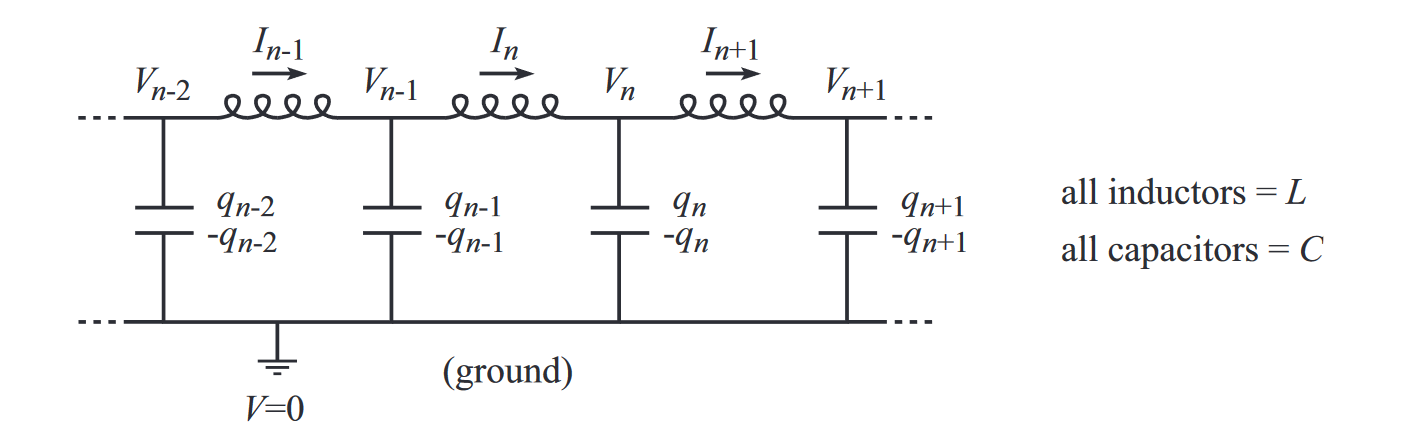
\includegraphics[width=\linewidth]{figures/circuit.png}
\end{figure}

There are three relevant facts:
\begin{enumerate}
    \item The charge on a capacitor is $Q = CV \implies q_n = CV_n$.
    \item The voltage across an inductor is $V = L(\dvi{I}{t}) \implies V_{n-1} - V_n = L(\dvi{I_n}{t})$.
    \item Conservation of charge yields $I_n - I_{n+1} = \dvi{q_n}{t}$.
\end{enumerate}
Our goal is to produce an equation for one of the three variables $q$, $I$, or $V$. This equation will turn out to be a wave equation, that is exactly the same for each variable. We could manipulate the above equations and then take the continuum limit to do this, but we will find that it is actually far easier to take the limit first and then manipulate the expressions.

If we let the width of the grid be $\Delta x$, then the above three facts become
\begin{align*}
    q &= CV \\
    -\pdv{V}{x}\Delta x &= L\pdv{I}{t} \\
    -\pdv{I}{x}\Delta x &= \pdv{q}{t}
\end{align*}
substituting $q=CV$ from the first equation into the third yields
\[ -\pdv{I}{x}\Delta x = C\pdv{V}{t} \]
Then, defining the inductance and capacitance per unit length as $L_0 \equiv L/\Delta x$ and $C_0 \equiv C/\Delta x$, we find the two equations
\[ -\pdv{V}{x} = L_0\pdv{I}{t} \quad\text{and}\quad -\pdv{I}{x} = C_0\pdv{V}{t} \]
Taking the space derivative of the first equation and the time derivative of the second, we find
\[ -\pdv[2]{V}{x} = L_0\frac{\partial ^2I}{\partial t\partial x}\quad\text{and}\quad -C_0\pdv[2]{V}{t} = \frac{\partial^2 I}{\partial x \partial t}\]
These can be set equal to each other to find
\[ \frac{1}{L_0}\pdv[2]{V}{x} = C_0\pdv[2]{V}{t}\]
or, rearranging slightly,
\[ \pdv[2]{V(x,t)}{t} = \frac{1}{L_0C_0}\pdv[2]{V(x,t)}{x} \]
this is the wave equation for a dispersionless wave with a speed
\[ c = \frac{1}{\sqrt{L_0C_0}}\]
Similar analyses show us that the exact same wave equation holds for $V$, $q$, and $I$.

Now, let's look at an actual coaxial cable. Consider a conducting wire inside a conducting cylinder, with vacuum in the region between them. Assume that the wire is somehow constrained to be in the middle of the cylinder. The cable has an inductance $L_0$ per unit length, in the same way that two parallel wires do. It also has a capacitance $C_0$ per unit length.

An arduous calculation shows that
\[ L_0 = \frac{\mu_0}{2\pi} \ln(r_2/r_1) \quad\text{and}\quad C_0 = \frac{2\pi\epsilon_0}{\ln(r_2/r_2)} \]
Thus, the wave speed is 
\[ v = \frac{1}{\sqrt{L_0C_0}} = \frac{1}{\mu_0\epsilon_0} \approx 3\times 10^8 \text{ m/s}\]
This is the speed of light! So the voltage, charge, and current waves all travel down the cable at the speed of light. And because there are electric and magnetic fields in the cable, these fields also undergo wave motion. Since the waves of these fields travel at the same speed as the original voltage wave, it is a good bet that electromagnetic waves have something to do with light. 
\section{The Wave Equation}
Maxwell's four equations govern all of electromagnetism, and here they are, in both differential and integral form:
\begin{align*}
    &\div \mbf E = \frac{\rho_E}{\epsilon_0} &&\oiint \mbf E \cdot \dd \mbf A = \frac{Q_E}{\epsilon_0} \\
    &\div \mbf B = \rho_B &&\oiint \mbf B \cdot \dd \mbf A = Q_B \\
    &\curl \mbf E = -\pdv{\mbf B}{t} + \mbf J_B &&\oint \mbf E \cdot \dd\mbf l = -\dv{\Phi_B}{t} + I_B \\
    &\curl \mbf B = \mu_0\epsilon_0 \pdv{\mbf E}{t} + \mu_0\mbf J_E &&\oint \mbf B \cdot \dd \mbf l = \mu_0\epsilon_0 \dv{\Phi_E}{t} + \mu_0 I_E
\end{align*}
If we erase the $\mu_0$'s and $\epsilon_0$'s here, which arise from the arbitrary definitions of our units, then these equations are symmetric in $\mbf E$ and $\mbf B$, save for a few minus signs. The $\rho$'s are the electric and (hypothetical) magnetic charge densities, and the $\mbf J$'s are the current densities. The $Q$'s are the charges enclosed by the surface that define the $\dd \mbf A$ integrals, and the $\Phi$'s are the field fluxes through the loops that define the $\dd\mbf l$ integrals.

No one has ever found an isolated magnetic charge, and there are various theoretical considerations that suggest they can't exist, at least in our universe. So we'll set $\rho_B$, $\mbf J_B$, and $I_B$ equal to zero from here on. This will make Maxwell's equations appear asymmetrical, but we'll soon be setting the analogous electric quantities equal to zero too. Thus, Maxwell's equations become
\begin{align*}
    &\div \mbf E = \frac{\rho_E}{\epsilon_0} &&\oiint \mbf E \cdot \dd \mbf A = \frac{Q_E}{\epsilon_0} \\
    &\div \mbf B = 0 &&\oiint \mbf B \cdot \dd \mbf A = 0 \\
    &\curl \mbf E = -\pdv{\mbf B}{t} &&\oint \mbf E \cdot \dd\mbf l = -\dv{\Phi_B}{t} \\
    &\curl \mbf B = \mu_0\epsilon_0 \pdv{\mbf E}{t} + \mu_0\mbf J_E &&\oint \mbf B \cdot \dd \mbf l = \mu_0\epsilon_0 \dv{\Phi_E}{t} + \mu_0 I_E
\end{align*}
In order, these laws are known as Gauss' Law, ``No magnetic monopoles," Faraday's law, and Ampere's law. Ampere's law includes the so-called ``displacement current" $\dvi{\Phi_E}{t}$.

Our goal is to derive the wave equation for the $\mbf E$ and $\mbf B$ fields in a vacuum. Since there are no charges in any kind of vacuum, we'll set $\rho_E$ and $\mbf J_E$ equal to zero from here on. And we'll only need the differential forms, so we now have
\begin{align*}
    \div  \mbf E &= 0 \\
    \div  \mbf B &= 0 \\
    \curl \mbf E &= -\pdv{\mbf B}{t} \\
    \curl \mbf B &= \mu_0\epsilon_0 \pdv{\mbf E}{t} 
\end{align*}
Taking the curl of the third of these equations, we find
\[ \curl(\curl \mbf E)  =-\curl \pdv{\mbf B}{t} \]
for the right side, we find
\begin{align*}
    -\curl \pdv{\mbf B}{t} &= -\pdv{t}\pqty{\curl \mbf B} \\
    &= -\pdv{t} \pqty{\mu_0\epsilon_0\pdv{\mbf E}{t}} \\
    &= -\mu_0\epsilon_0 \pdv[2]{\mbf E}{t}
\end{align*}
for the left side, we use the handy ``BAC-CAB" formula
\[ \mbf A \times (\mbf B \times \mbf C) = \mbf B(\mbf A \cdot \mbf C) - \mbf C(\mbf A\cdot \mbf B)\]
which tells us that
\begin{align*}
    \curl(\curl \mbf E) &= \grad(\div \mbf E) - \mbf E(\div \grad) \\
    &= \mbf 0 - \grad^2\mbf E = -\grad^2\mbf E
\end{align*}
Thus, we find that
\[ \boxed{\pdv[2]{\mbf E}{t} = \frac{1}{\mu_0\epsilon_0} \grad^2\mbf E} \]
We could have instead eliminated $\mbf E$ instead of $\mbf B$, which would give us exactly the same wave equation (since Maxwell's equations are symmetric),
\[ \boxed{\pdv[2]{\mbf B}{t} = \frac{1}{\mu_0\epsilon_0} \grad^2\mbf B} \]
The speed of the waves is still given by the square root of the coefficient on the right hand side of the equation (this isn't completely obvious, since we're now in three dimensions instead of one, but we'll justify this below). So the speed of electromagnetic waves is also equal to the speed of light.

The critical observation here is that these waves do \textbf{not} need a medium to propogate--we derived them under the assumption that we are in a vacuum. This is a fundamentaly new property that has not been present in any of the waves we previously studied.

The wave equation is actually three wave equations, one for each spatial dimension (we could write these equations for either $\mbf E$ and $\mbf B$, as they are identical. I arbitrarily chose to use $\mbf E$)
\begin{align*}
    \pdv[2]{E_x}{t} &= \frac{1}{\mu_0\epsilon_0} \pqty{\pdv[2]{E_x}{x} + \pdv[2]{E_x}{y} + \pdv[2]{E_x}{z}} \\
    \pdv[2]{E_y}{t} &= \frac{1}{\mu_0\epsilon_0} \pqty{\pdv[2]{E_y}{x} + \pdv[2]{E_y}{y} + \pdv[2]{E_y}{z}} \\
    \pdv[2]{E_z}{t} &= \frac{1}{\mu_0\epsilon_0} \pqty{\pdv[2]{E_z}{x} + \pdv[2]{E_z}{y} + \pdv[2]{E_z}{z}}
\end{align*}
As far as the wave equation is concerned, these components are completely independent of each other; their amplitudes, frequencies, and phases need not have anything to do with each other.

However, there is more information contained in Maxwell's equations than in the wave equation. We will see that Maxwell's equations do indeed further constrain the form of these waves.
\subsection*{Index of Refraction}
In a dielectric, the vacuum quantities $\mu_0$ and $\epsilon_0$ in Maxwell's equations are replaced by new values, $\mu$ and $\epsilon$. Our derivation of the wave equation for electromagnetic waves in a dielectric proceeds in exactly the same way as for the vacuum case above, except with $\mu_0\to \mu$ and $\epsilon_0\to\epsilon$. The therefore end up with a wave speed equal to
\[ v = \frac{1}{\sqrt{\mu \epsilon}} \]
The \textbf{index of refraction}, $n$, of a dielectric, is defined as $v = c/n$, where $c$ is the speed of light in a vacuum. We therefore have
\[ n = \frac{c}{v} \implies \boxed{n = \sqrt{\frac{\mu\epsilon}{\mu_0\epsilon_0}}}\]
Since it happens that $\mu \approx \mu_0$ for most dielectrics, we have
\[ n \approx \sqrt{\frac{\epsilon}{\epsilon_0}}\]
Since we must always have $v \le c$, then $n \ge 1$. Thus, $\epsilon \ge \epsilon_0$.

Strictly speaking, Maxwell's equations with $\mu_0$ and $\epsilon_0$ work in any medium. But if we are not in a vacuum, then induced charges and currents may arise.

There are two types of charges. First are so-called \textbf{free charges}, which are additional charges which we can plop down in a material. This is what we typically think of when we think of charge. But there are also \textbf{bound charges}, which are the effective charges that are produced when polar molecules align themselves to ``shield" the free charges.

For instance, if we place a positive free charge $q_\text{free}$ in a material, then the nearby polar molecules will align themselves so that their negative ends form a negative layer around the free charge. The net charge inside a Gaussian surface around the charge is therefore less than $q$. Call it $q_\text{net}$. Maxwell's first equation is then $\div\mbf E = \rho_\text{net}/\epsilon_0$. However, it is generally much easier to work with $\rho_\text{free}$ than with $\rho_\text{net}$, so let's define $\epsilon$ with $\rho_\text{net}/\rho_\text{free} = \epsilon_0 / \epsilon$. Maxwell's first equation can then be written
\[ \div \mbf E = \frac{\rho_\text{free}}{\epsilon} \]
So the electric field in the material around a point charge is less than it would be in a vacuum, by a factor of $\epsilon_0/\epsilon$. In a dielectric, the fact that $\epsilon \ge \epsilon_0$ is consistent with the fact that the index of refraction $n\ge 1$, which is in turn consistent with the fact that $v\le c$.

A similar occurrence also happens with currents. There can be \textbf{free currents}, which are the normal ones we think about. But there can also be \textbf{bound currents}, which arise from tiny current loops of electrons spinning around within their atoms. This is a little harder to visualize than with the charges, but let's just accept here that the fourth of Maxwell's equations becomes $\curl \mbf B = \mu\epsilon \, \pdvi{\mbf E}{t} + \mu \mbf J_\text{free}$. But as mentioned above, $\mu\approx \mu_0$, so this distinction isn't usually very important.

The above modified expressions for Maxwell's equations are correct if we're dealing with a single medium. But if we have two or more mediums, the correct way to write the equations is to multiply the first equation by $\epsilon$ and divide the fourth by $\mu$. The collection of all four Maxwell's equations is then
\begin{align*}
    \div \mbf D &= \rho_\text{free} \\
    \div \mbf B &= 0 \\
    \curl \mbf E &= -\pdv{\mbf B}{t} \\
    \curl \mbf H &= \pdv{\mbf D}{t} + \mbf J_\text{free}
\end{align*}
where $\mbf D \equiv \epsilon \mbf E$ and $\mbf H \equiv \mbf B/\mu$. $\mbf D$ is called the \textbf{electric displacement vector}, and $\mbf H$ goes by many names, including simply (confusingly) the ``magnetic field." 
\section{Form of the Waves}
\subsection*{Wavevectors}
What is the dispersion relation associated with the above wave equation? That is, what is the relation of the frequency and wavenumber? More precisely, what is the dispersion relation for each component of $\mbf E$? All of the components are in general functions of the three spatial coordinates and time. By the same reasoning as in the two-dimensional case, we know that we can Fourier-decompose the function $E_x(x,y,z,t)$ into exponentials of the form
\[ Ae^{i(k_xx+k_yy+k_zz-\omega t)} \equiv Ae^{i(\mbf k \cdot \mbf r - \omega t)}\]
where $\mbf r = (x,y,z)$ and $\mbf k = (k_x, k_y, k_z)$. And likewise for the three components of $\mbf B$.

These are traveling waves, although we can form combinations of them to produce standing waves.

$\mbf k$ is known as the \textbf{wavevector}. As we'll see, the magnitude $k \equiv \abs{\mbf k}$ plays exactly the same role that $k$ played in the 1-D case. That is, $k$ is the wavenumber. We still have $k = 2\pi/\lambda$. We will also see that $\mbf k$ points in the direction of the propagation of the wave. 

Plugging the exponential guess into the wave equation yields
\[ -\omega^2 = \frac{1}{\mu_0\epsilon_0}(-k_x^2-k_y^2-k_z^2) \implies \omega^2 = \frac{k^2}{\mu_0\epsilon_0} \implies \boxed{\omega = ck} \]
When we go through the same procedure for the other components of $\mbf E$ and $\mbf B$, the $A$ coefficient can be different in each case. Technically, the wave equation does not say that $\mbf k$ and $\omega$ must be equal for all six, but Maxwell's equations do. So $\mbf k$ and $\omega$ must be the same for all six components of $\mbf E$ and $\mbf B$.

If we then collect all of the constants into two constant vector $\mbf E_0$ and $\mbf B_0$ to represent the amplitudes of the waves, we have
\[ \boxed{\mbf E = \mbf E_0 e^{i(\mbf k \cdot \mbf r - \omega t)} \quad\text{and}\quad \mbf B = \mbf B_0 e^{i(\mbf k\cdot \mbf r - \omega t)}} \]
These vectors $\mbf E_0$ and $\mbf B_0$ may be complex. If they have an imaginary part, it will produce a phase in the cosine function when we take the real part of the above exponentials. 

Since $\mbf E$ and $\mbf B$ depend on $\mbf r$ only through the dot product $\mbf k \cdot \mbf r$, $\mbf E$ and $\mbf B$ are constant along the level surfaces defined by $\mbf k \cdot \mbf r = C$. These surfaces turn out to be planes orthogonal to $\mbf k$, since if we take any two points on them $\mbf r_1$ and $\mbf r_2$, we have $\mbf k \cdot (\mbf r_1 - \mbf r_2) = 0$, which defines a plane with normal vector $\mbf k$. As far as $\mbf E$ and $\mbf B$ are concerned, every point on these planes is equivalent.

How do these wavefronts move as time goes by? Since they are normal to $\mbf k$, they must move in the direction of $\mbf k$. But how fast to they move? The dot product $\mbf k \cdot \mbf r$ equals $kr\cos\theta$, where $\theta$ is the angle between $\mbf k$ and some given $\mbf r$. This is simply $k$ times the projection of $\mbf r$ along $\mbf k$. Rotating our coordinate system so that the new $x'$ axis points in the $\mbf k$ direction, then the projection $r\cos\theta$ is simply $x'$, so the phase $\mbf k\cdot \mbf r - \omega t = kx' - \omega t$.

We have essentially reduced this to a 1-D problem, so we can carry over all of out 1-D results. In particular, the phase velocity is $v= \omega/k$, which we know also equals $c$.
\subsection*{Further Constraints}
Many of the waves that satisfy the wave equation we previously found do \textbf{not} satisfy Maxwell's equations. We will explore the restrictions we must impose to make this no longer the case.
\begin{enumerate}
    \item Because $\div \mbf E = 0$, we must have 
    \[ \pdv{E_x}{x} + \pdv{E_y}{y} + \pdv{E_z}{z} = 0\]
    But with $\mbf E = \mbf E_0 e^{i(\mbf k \cdot \mbf r - \omega t)}$, this becomes
    \[ ik_xE_x + ik_y E_y + ik_z E_z = 0\]
    so $\mbf E \cdot \mbf k = 0$ and thus $\mbf E$ is perpendicular to $\mbf k$.
    \item $\div \mbf B = 0$ gives the same result for $\mbf B$, namely, $\mbf B \cdot \mbf k = 0$ and so $\mbf B$ is perpendicular to $\mbf k$.
    \item With $\curl\mbf E = -\pdv{\mbf B}{t}$, we see that 
    \begin{align*}
        \pqty{\pdv{x}, \pdv{y}, \pdv{z} }\times \mbf E &= - \pdv{\mbf B}{t} \\
        i\mbf k \times \mbf E &= -(-i\omega )\mbf B \\
        \mbf k \times \mbf E &= \omega \mbf B
    \end{align*}
    This tells us that $\mbf B$ and $\mbf E$ are perpendicular. Since we already know that $\mbf k$ and $\mbf E$ are perpendicular, the magnitude of $\mbf k \times \mbf E$ is just $kE$. So we have
    \[ kE = \omega B \implies E = \frac{\omega}{k} B = cB \implies \boxed{E = cB} \]
    This is a useful relation, but it is only valid for a single traveling wave. If we take the sum of two waves with different $\mbf k$ vectors, then the sum dosn't satisfy $\mbf k \times \mbf E = \omega \mbf B$ for any particular vector $\mbf k$.
    \item Because $\curl \mbf B = (1/c^2) \; \pdvi{\mbf E}{t}$, the same procedure can be used to give
    \[ B = \frac{1}{c}E\]
    this gives us no new information.
\end{enumerate}
All of the above results can be summarized:
\[ \boxed{\mbf E \perp \mbf B \quad \mbf E \perp \mbf k \quad \mbf B \perp \mbf k \quad E = cB}\]
With the convention we have established, the pair $\mbf E$, $\mbf B$, and $\mbf k$ form a ``righthanded" triplet--that is, $\mbf E \times \mbf B$ points in the same direction of $\mbf k$, and so we can use the right hand rule.

Suppose that the wavevector $\mbf k = k\zhat$ and suppose $\mbf E$ points in the $x$ direction. So, the electric field vector is given by $\mbf E = E_0e^{i(\mbf k \cdot \mbf r - \omega t+\phi)}\xhat$, where the phase has come from the fact that we have taken $E_0$ to be real, so we must absorb its phase into the exponential. Since the wave propagates in the $z$ direction, we take $\mbf r = (0,0,z)$. Then, the actual wave comes from taking the real part of this expression,
\[ \mbf E = \xhat E_0\cos(kz -\omega t + \phi)\]
By the right hand rule, we see that $\mbf B$ points in the $y$ direction, and its magnitude is given by $B = \frac{1}{c}E$. Thus,
\[ \mbf B = \zhat \frac{E_0}{c}\cos(kz - \omega t+\phi) \]
\subsection*{Standing waves}
To generate a standing wave, we do the usual method of adding two waves with equal amplitudes traveling in opposite directions. Let $\mbf E_1 = \xhat E_0\cos(kz-\omega t)$ and $\mbf E_2 = \xhat E_0\cos(-kz-\omega t)$. We then obtain
\[ \mbf E = \mbf E_1 + \mbf E_2 = \xhat E_0(\cos(kz-\omega t)+\xhat E_0\cos(-kz-\omega t))\]
With the sum of cosines identity, this becomes
\[ \mbf E = \xhat 2E_0\cos(kz)\cos(\omega t)\]
This is indeed a standing wave, since all $z$ values have the same phase with respect to time. Here, we must be careful. The relationship $\omega \mbf B = \mbf k \times \mbf E$ is \textbf{not} true here, since that only holds for single waves--this is the superposition of two waves. In fact, there isn't even one single $\mbf k$ vector for $\mbf E$, since the wavevector for $\mbf E_1$ and $\mbf E_2$ are pointing in opposite directions.

There are two primary ways to find $\mbf B$. The first is the easiest, and it is to write $\mbf B = \mbf B_1 + \mbf B_2$ where $\mbf B_1$ is the field associated with $\mbf E_1$ and $\mbf B_2$ is associated with $\mbf E_2$. We can then use the relationship $\omega \mbf B = \mbf k \times \mbf E_1$ to find $\mbf B_1$, $\mbf B_2$. For $\mbf B_1$, we have
\begin{align*}
    \mbf B_1 &= \frac{1}{\omega}(\mbf k_1 \times \mbf E_1) \\
    &= \frac{1}{\omega} \pqty{k\zhat } \times \pqty{\xhat E_0 \cos(kz-\omega t)} \\
    &= \yhat\frac{E_0}{c}\cos(kz-\omega t) 
\end{align*}
And for $\mbf B_2$, we have
\begin{align*}
    \mbf B_2 &= \frac{1}{\omega}(\mbf k_2 \times \mbf E_2) \\
    &= \frac{1}{\omega}\pqty{-k\zhat}\times \pqty{\xhat E_0 \cos(-kz-\omega t)} \\
    &= -\yhat\frac{E_0}{c}\cos(-kx-\omega t)
\end{align*}
Then, the total magnetic field is
\begin{align*}
    \mbf B &= \mbf B_1 + \mbf B_2 = \yhat \frac{E_0}{c}[\cos(kz-\omega t)-\cos(-kz-\omega t) \\
    &= \yhat \frac{2E_0}{c}\sin(kz)\sin(\omega t)
\end{align*}
A second method is to apply Maxwell's equations directly. Using $\curl \mbf E = -\pdvi{\mbf B}{t}$, write
\begin{align*}
    \curl \mbf E = \yhat \pdv{E_x}{z} = -\yhat 2kE_0\sin(kz)\cos(\omega t)
\end{align*}
So $-\pdvi{\mbf B}{t} = -\yhat 2kE_0\sin(kz)\cos(\omega t)$. Thus, (ignoring any constant of integration, which we know must be zero),
\[ \mbf B = \yhat \frac{2kE_0}{\omega}\sin(kz)\sin(\omega t) = \yhat\frac{2E_0}{c}\sin(kz)\sin(\omega t)\]
Notice that in this case, the $\mbf E$ and $\mbf B$ are exactly $90^\circ$ out of phase in both time and space, which is different than the single traveling wave case, where $\mbf E$ and $\mbf B$ are perfectly in phase. 
\section{Energy}
\subsection*{The Poynting Vector}
It can be shown that the energy density of an electromagnetic field is given by
\[ \mcl E = \frac{1}{2}\epsilon_0 E^2 + \frac{1}{2\mu_0} B^2\]
We can equivalently write this as 
\[ \mcl E = \frac{1}{2}\epsilon_0 \mbf E \cdot \mbf E + \frac{1}{2\mu_0} \mbf B \cdot \mbf B\]
which allows us to use the product rule to state
\begin{align*}
    \pdv{\mcl E}{t} = \epsilon_0 \pqty{\mbf E \cdot \pdv{\mbf E}{t}} + \frac{1}{\mu_0}\pqty{\mbf B \cdot \pdv{\mbf B}{t}}
\end{align*}
Using Maxwell's equations, we can rewrite to find
\begin{align*}
    \pdv{\mcl E}{t} &= \epsilon_0\pqty{\mbf E \cdot \pqty{\frac{1}{\mu_0\epsilon_0}\curl \mbf B}} + \frac{1}{\mu_0}\pqty{\mbf B \cdot (-\curl \mbf E)} \\
    &= \frac{1}{\mu_0} \pqty{\mbf E \cdot (\curl \mbf B) - \mbf B \cdot (\curl \mbf E)}
\end{align*}
Using the vector calculus identity $\mbf B\cdot(\curl \mbf A) - \mbf A \cdot(\curl \mbf B) = \div(\mbf A\times \mbf B)$, we find
\[ \pdv{\mcl E}{t} = \frac{1}{\mu_0} \div(\mbf B \times \mbf E)\]
Then, to get the total energy $W_V$ (we've run out of $E$s to use) in a region $V$ in space, we can integrate this over $V$:
\begin{align*}
    \pdv{W_V}{t} &= \iiint\limits_V \pdv{\mcl E}{t} \dd V' = \frac{1}{\mu_0}\iiint\limits_V \div(\mbf B\times \mbf E) \dd V' \\
    &= \frac{1}{\mu_0}\oiint\limits_{\partial V} (\mbf B \times \mbf E)\cdot \dd \mbf A
\end{align*}
Standard convention tells us that $\dd \mbf A$ is the outward-pointing area vector, but we will make a slight change in notation. Define the inward-pointing area vector as $\dd \mbf A_\text{in} \equiv -\dd \mbf A$, which allows us to write
\[ \pdv{W_v}{t} = \frac{1}{\mu_0}\oiint\limits_{\partial V} (\mbf E\times \mbf B)\cdot \dd \mbf A_\text{in}\]
We define the \textbf{Poynting vector} as
\[ \boxed{\mbf S \equiv \frac{1}{\mu_0} \mbf E\times \mbf B}\]
Which can be interpreted as giving the flux of energy \textbf{into} a region.
\subsection*{Traveling Waves}
Let's look at the energy density $\mcl E$ and the Poynting vector $\mbf S$ for a traveling wave. For a traveling wave, $B = (1/c)E$, so
\[ \mcl E = \frac{1}{2}\epsilon_0 E^2 + \frac{1}{2\mu_0 c^2} E^2 = \epsilon_0E^2 \]
The Poynting vector for a traveling wave is 
\[ \mbf S = \frac{1}{\mu_0 c} E^2   \mbf{\hat k} = c\epsilon_0 E^2 \mbf{\hat k} = c\mcl E \mbf{\hat k} \]
This is essentially saying that the energy density $\mcl E$ moves along the wave, at the same speed $c$ as the wave. So the energy per unit area per unit time that crosses a given surface is $c\mcl E$.

If we have a sinusoidal traveling wave of the form
\[ \mbf E = \xhat E_0 \cos(kz-\omega t +\phi) \quad\text{and}\quad \mbf B = \yhat (E_0/c)\cos(kz-\omega t+\phi) \]
we find an energy density and Poynting vector of
\[ \mcl E = \epsilon_0 E_0^2\cos^2(kz-\omega t +\phi) \quad\text{and}\quad \mbf S = \zhat c\epsilon_0E_0^2\cos^2(kz-\omega t+\phi) \]
Since the average value of $\cos^2$ over one period is $1/2$, we have
\[ \mcl E_\text{avg} = \frac{1}{2}\epsilon_0 E_0^2 \quad\text{and} \quad S_\text{avg} = \frac{1}{2}c\epsilon_0E_0^2\]
$S_\text{avg}$, the average magnitude of the Poynting vector, is known as the \textbf{intensity} of the wave. 
\subsection*{Standing Waves}
Let's now look at the energy density $\mcl E$ and Poynting vector $\mbf S$ for a standing wave. Consider a standing wave of the form
\[ \mbf E = \xhat A\cos(kz)\cos(\omega t) \quad\text{and}\quad \mbf B = \yhat (A/c)\sin(kz)\sin(\omega t)\]
Then, the energy density is
\begin{align*}
    \mcl E &= \frac{1}{2}\epsilon_0 A^2 \cos^2(kz)\cos^2(\omega t) + \frac{1}{2\mu_0}\frac{A^2}{c^2}\sin^2(kz)\sin^2(\omega t) \\
    &= \frac{1}{2}\epsilon_0 A^2\pqty{\cos^2(kz)\cos^2(\omega t) + \sin^2(kz)\sin^2(\omega t)}
\end{align*}
If we take the average over a whole cycle in time, then each of the $\cos^2(\omega t)$ and $\sin^2(\omega t)$ terms turn into $1/2$. So the time average of $\mcl E$ is given by
\[ \mcl E_\text{avg} = \frac{1}{4}\epsilon_0 A^2\pqty{\cos^2(kz)+\sin^2(kz)} = \frac{1}{4}\epsilon_0 A^2 \]
Notice that this doesn't depend on $z$; a standing wave has a uniform average energy density. 

The Poynting vector for our wave is given by
\begin{align*}
    \mbf S &= \frac{1}{\mu_0}\mbf E\times\mbf B = \zhat \frac{1}{\mu_0}\frac{A^2}{c}\cos(kz)\cos(\omega t)\sin(kz)\sin(\omega t) 
\end{align*}
At any given $t$, the spatial average value of $\mbf S$ is zero (because $\cos(kz)$ and $\sin(kz)$ are orthogonal), so there is no net energy flow in a standing wave. This makes sense with our intuition. Similarly, for any given $z$, the time average value is zero.

Note that this does \textbf{not} mean that the Poynting vector is zero at any given $x,t$. This just means that all of the (nonzero) values of the Poynting vector average to zero.
\section{Momentum}
Electromagnetic waves, unlike other waves we have studied, carry momentum. 

A quick argument that demonstrates why an electromagnetic wave (that is, light) carries momentum is the following argument from relativity. The relativistic relation between a particle's mass, energy, and momentum is as follows: $E^2 = p^2c^2 + m^2c^4$. For a massless particle (we will accept here that photons have $m=0$), we have $E = pc$. Thus, the momentum is $p = E/c$.

A different argument that does not rely on relativity follows. Consider a particle with charge $q$ that is free to move around in a material. This particle will experience a Lorentz force $\mbf F = q(\mbf E + \mbf v \times \mbf B)$ from the fields that make up the wave. The particle will also lose energy due to the damping forces in the material and from the radiation of the particle.

Consider a traveling wave that propagates in the $z$ direction, the $\mbf E$ field points in the $x$ direction, and the $\mbf B$ field points in the $y$ direction. The general motion of the particle will be very complicated, but it will suffice to consider the field parallel to the $\mbf E$ field (i.e. the field in the $x$ direction). 

Due to the oscillation of $\mbf E$, the particle will (mainly) oscillate back and forth in the $x$ direction. We don't know the phase, but we can in general write it as the sum of a component perfectly in phase with $\mbf E$ and and part of it will be perfectly out of phase with $\mbf E$. Denote the component of the velocity parallel to $\mbf E$ with $\mbf v_E$. Since $\mbf v_E$ and $\mbf B$ switch signs at the same time, $\mbf v_E\times \mbf B$ always points along the wavevector $\mbf k$. Thus there is always a net force forward. 

Therefore, the particle picks up some forward momentum from the wave. In a small time $\dd t$, the magnitude of the change in momentum is given by
\[ \abs{\dd \mbf p} = \abs{q\mbf v_E\times \mbf B\dd t} = \abs{qv_EB\dd t} = \frac{qv_EE \dd t}{c}\]
The only work done on the particle is by the electric field, so 
\[ \dd W = \mbf F_E \cdot \dd \mbf x = qEv_E\dd t\]
Therefore,
\[ \abs{\dd \mbf p} = \frac{\dd W}{c} \]
In other words, the change in (the magnitude of the) momentum from the wave is equal to $1/c$ times the change in energy from the wave. This result holds in the non-infinitesimal case as well, so
\[ \abs{\mbf p} = \frac{W}{c} \]
Another way of writing this equation is that
\[ \frac{1}{A}\abs{\dv{\mbf p}{t}} = \frac{1}{Ac}\dv{W}{t}\]
where $A$ is the cross-sectional area of the wave under consideration. The left hand side of this equation has units of force/area, and represents the pressure on the area $A$. We can also notice that the right hand side is equal to $|\mbf S|/c$. Thus, the pressure from an electromagnetic wave, called the \textbf{radiation pressure}, is given by
\[ \frac{|\mbf S|}{c} = \frac{|\mbf E\times \mbf B|}{\mu_0 c} = \frac{E^2}{\mu_0c^2}\]
\section{Polarization}
 % electromagnetic waves
\end{document}